%% LaTeX2e class for student theses
%% thesis.tex
%% 
%% Karlsruhe Institute of Technology
%% Institute for Program Structures and Data Organization
%% Chair for Software Design and Quality (SDQ)
%%
%% Dr.-Ing. Erik Burger
%% burger@kit.edu
%%
%% See https://sdqweb.ipd.kit.edu/wiki/Dokumentvorlagen
%%
%% {$HeadURL$}
%% {$LastChangedDate$}
%% {$LastChangedRevision$}
%% {$LastChangedBy$}

%% Available page modes: oneside, twoside
%% Available languages: english, ngerman
%% Available modes: draft, final (see README)
\documentclass[oneside, ngerman, final]{sdqthesis}

%% ---------------------------------
%% | Information about the thesis  |
%% ---------------------------------

%% Name of the author
\author{Nina Zimbel}

%% Title (and possibly subtitle) of the thesis
\title{Prozedurale Generierung von Wirbeltierskeletten}

%% Type of the thesis 
\thesistype{Master's Thesis}

%% Change the institute here, ``IPD'' is default
 \myinstitute{Institute for Computer Graphics}

%% You can put a logo in the ``logos'' directory and include it here
%% instead of the SDQ logo
% \grouplogo{myfile}
%% Alternatively, you can disable the group logo
% \nogrouplogo

%% The reviewers are the professors that grade your thesis
\reviewerone{Prof. Dr.-Ing. Carsten Dachsbacher}
\reviewertwo{Prof. ?}

%% The advisors are PhDs or Postdocs
\advisorone{Dr. Johannes Schudeiske}
%% The second advisor can be omitted
%\advisortwo{M.Sc. D}

%% Please enter the start end end time of your thesis
\editingtime{xx. Month 20XX}{xx. Month 20XX}

\settitle

%% --------------------------------
%% | Settings for word separation |
%% --------------------------------

%% Describe separation hints here.
%% For more details, see 
%% http://en.wikibooks.org/wiki/LaTeX/Text_Formatting#Hyphenation
\hyphenation{
% me-ta-mo-del
}

%% --------------------------------
%% | Bibliography                 |
%% --------------------------------

%% Use biber instead of BibTeX, see README
\usepackage[citestyle=numeric,style=numeric,backend=biber]{biblatex}
\addbibresource{bibliography.bib}

%% ====================================
%% ====================================
%% ||                                ||
%% || Beginning of the main document ||
%% ||                                ||
%% ====================================
%% ====================================
\begin{document}

%% Set PDF metadata
\setpdf

%% Set the title
\maketitle

%% The Preamble begins here
%\frontmatter

%\input{sections/declaration.tex}

\setcounter{page}{1}
\pagenumbering{roman}

%% ----------------
%% |   Abstract   |
%% ----------------
 
%% For theses written in English, an abstract both in English
%% and German is mandatory.
%%
%% For theses written in German, a German abstract is sufficient.
%%
%% The text is included from the following files:
%% - sections/abstract

%\includeabstract

%% ------------------------
%% |   Table of Contents  |
%% ------------------------
%\tableofcontents

%\listoffigures
%\listoftables

%% -----------------
%% |   Main part   |
%% -----------------

\mainmatter

%%-------------------
%-------------------
\chapter{Einleitung}

Wirbeltiere sind allgegenwärtig, sowohl im alltäglichen Leben, als auch in Computerspielen und Filmen. Es besteht also ein stetiger Bedarf an 3D-Modellen von Wirbeltieren. Dieser wird in den meisten Fällen durch Künstler gedeckt, die viel Zeit und Arbeit in die Modelle stecken. Algorithmen, die diese Abläufe vereinfachen könnten, beispielsweise durch prozedurale Generierung, gibt es nicht viele.

% Ziel
Das Ziel dieser Arbeit ist es den Arbeitsaufwand der Künstler zu verringern, indem eine Möglichkeit geschaffen wird Wirbeltierskelette automatisiert zu generieren. Diese Skelette können dann die Grundlage für die Modellierung eines kompletten Wirbeltiers bilden.
Einerseits können sie dabei als Inspiration dienen. Sie können einen Anhaltspunkt zu Körperform und Proportionen bieten und zu möglichen Bewegungsabläufen. Außerdem kann schnell eine große Auswahl an Skeletten generiert werden.\\
Andererseits können die Skelette eine Grundlage für Modelle bilden, die zusätzlich auch Muskeln und Haut simulieren.
In beiden Fällen darf das Modell nicht zu abstrakt sein, da es sonst zu wenig Informationen zum Aufbau des konkreten Tiers liefert.\\
Es soll also ein Skelett generiert werden, dass genug Knochen enthält um realistisch zu wirken, aber auch nicht zu viele um den Aufwand für die Generierung und die Programmierung des Algorithmus im Rahmen zu halten.

% Warum nur Wirbeliere?
Der Grund dafür, dass sich diese Arbeit auf Wirbeltierskelette einschränkt ist, dass der Skelettaubau von Wirbeltieren nicht zu stark variiert. 
Je mehr Details betrachtet werden, desto mehr Unterschiede gibt es, aber der grobe Aufbau ist bei allen Wirbeltieren sehr ähnlich. Die Grundlagen zur Biologie der Wirbeltiere, die für diese Arbeit notwendig sind, werden in Kapitel \ref{chapter:biology} vorgestellt, die technischeren Grundlagen in Kapitel \ref{chapter:basics}.

% Methoden+Aufbau
Die wichtigsten Schritte des Algorithmus werden im Folgenden kurz angerissen, um einen Überblick über die Arbeit zu geben.
Die Datengrundlage für den Algorithmus schafft eine \emph{Principal Component Analyis} (Hauptkomponentenanalyse) auf annotierten 2D-Skelett"-bildern (Kapitel \ref{chapter:pca}). 
Die Knochen des Skeletts werden dann mit Hilfe einer kontextfreien Grammatik generiert und gleichzeitig angeordnet (Kapitel \ref{chapter:skeleton_generation}). 
Zum Schluss wird aus existierenden 3D-Modellen von einzelnen Knochen ein 3D-Modell des generierten Skeletts erstellt (Abschnitt \ref{bone_models})).\\
Zunächst generiert der Algorithmus zufällige Skelette. Es werden aber auch Benutzereingaben, \zb zur Anzahl der Extremitäten, berücksichtigt oder Variationen zu schon bestehenden Skeletten generiert (Kapitel \ref{chapter:additional_features}). \\
Zusätzliche Informationen zu Implementierungsdetails sind in Kapitel \ref{chapter:implementation_detail} zu finden und abgerundet wird die Arbeit mit Fazit und Ausblick in Kapitel \ref{chapter:conclusion}.

% Aufbau der Arbeit
% In Kapitel \ref{chapter:biology} werden zunächst einige Grundlagen zur Biologie der Wirbeltiere vorgestellt, die später zum Verständnis des Algorithmus nötig sind. Die technischeren Grundlagen werden in Kapitel \ref{chapter:basics} erklärt.\\
% Kapitel \ref{chapter:pca} widmet sich der \emph{Principal Component Analyis}. Es wird beschrieben auf welchen Daten und mit welchen Ergebnissen sie im Rahmen des Algorithmus angewandt wird. Diese Analyse ist auch der erste Schritt des Algorithmus, der in Kapitel \ref{chapter:skeleton_generation} ausführlich beschrieben wird. Zusätzliche Funktionen, wie das Laden und Speichern von Skeletten oder die Erzeugung von Variationen zu gespeicherten Skeletten werden in Kapitel \ref{chapter:additional_features} vorgestellt.
% Kapitel \ref{chapter:implementation_detail} versammelt alle Details zur Implementierung und abgerundet wird die Arbeit mit Fazit und Ausblick in Kapitel \ref{chapter:conclusion}.




\chapter{Bisherige Arbeiten}

%-------------
\section{Ziva}

\begin{itemize}
 \item Ziva VFX Maya Plugin zur Erstellung von Charakteren und Simulation von biomechanischen Bewegungen \url{https://zivadynamics.com/}
 \item Charaktererstellung in Ziva beginnt mit der Modellierung des Skeletts. Knochen mit Animationen werden als Alembic-Datei gespeichert und dann in "`Ziva-Knochen"' konvertiert. \url{https://discover.therookies.co/2019/06/01/vfx-in-9-steps/}
\end{itemize}

%---------------------------
\section{ZSpheres in Zbrush}

\begin{itemize}
 \item \url{http://docs.pixologic.com/user-guide/3d-modeling/modeling-basics/creating-meshes/zspheres/},\\ Beispielvideo: \url{https://www.youtube.com/watch?v=Wl0XK6ggUOA}
 \item Möglichkeit ein "`Skelett"' aus Kugeln zu erstellen. Definiert aber eher die grobe Außenhaut mit Zusatzinformationen dazu wo die Gelenke sind.
\end{itemize}

%----------------------
\section{3DS MAX Biped}

\begin{itemize}
 \item \url{https://knowledge.autodesk.com/support/3ds-max/learn-explore/caas/CloudHelp/cloudhelp/2019/ENU/3DSMax-Character-Animation/files/GUID-2F6BC5D1-DD45-4C2E-AC3A-D8C6E0F5DEB1-htm.html}
 \item Möglichkeit Skelett in einen fertig modellierten Körper einzupassen. 
 \item Skelette sind schon vorgefertigt.
 \item v.a. für menschliche Skelette, aber auch (limitiert) anpassbar auf Tiere
\end{itemize}

%---------------------------------
\section{Forensik und Archäologie}

\begin{itemize}
 \item forensische Gesichstrekonstruktion ist spezialisiert auf Menschen und verwendet Zusatzinformationen wie Stockfotos von Gesichtsmerkmalen (\url{https://en.wikipedia.org/wiki/Forensic_facial_reconstruction})
 \item Rekonstruktion von Tieren in der Archäologie anhand des Skeletts v.a. durch Künstler (?)
\end{itemize}


%----------------------
\section{No Man's Sky}

\begin{itemize}
 \item Webseite \cite{NoMansSky}
 \item "`For creatures, basic templates of creatures that exist on the Earth were created and then manipulated by the system, changing everything from height, weight, bone density, voice pitch, what it eats, and its behaviors, even creating variation within the species."' (\url{https://nomanssky.fandom.com/wiki/Biology})
 \item "`Creatures were often generated by mixing and matching random parts from a library, and then adjusting the underlying skeleton so that the creature appeared realistic; a creature with a tiny body could not support a giant head, for example."' (\url{https://en.wikipedia.org/wiki/Development_of_No_Man\%27s_Sky})
 \item Zunächst Generierung von äußerem 3D-Modell, dann Anpassung der Knochen.
\end{itemize}

%-----------------
%-----------------
\chapter{Biologie}

\begin{itemize}
 \item "`Wirbeltiere (Vertebrata) [\dots] Von vielen Zoologen wird heute der Begriff Schädeltiere (Craniota) für dieses Taxon bevorzugt. Diese Auffassung berücksichtigt, dass die Rundmäuler, wie auch einige andere Wirbeltiere, als Achsenskelett keine Wirbelsäule, sondern eine Chorda dorsalis haben. Doch allen Wirbeltieren gemein ist ein verknöcherter oder knorpeliger Schädel; sein Vorhandensein gehört somit zu den gemeinsam abgeleiteten Merkmalen (Synapomorphien) dieser Chordaten-Gruppe."' (\url{https://de.wikipedia.org/wiki/Wirbeltiere}) $\rightarrow$ Beschränkung auf Schädeltiere mit Wirbelsäule
 \item "`Dem Skelett der Wirbeltiere sind viele Gemeinsamkeiten ansehbar, trotzdem unterscheidet es sich, je nach Lebensraum und Anforderungen, teilweise erheblich. Mit diesen Gemeinsamkeiten und Unterschieden beschäftigt sich die Vergleichende Anatomie."' (\url{https://de.wikipedia.org/wiki/Skelett#Wirbeltiere}) Notizen zu \cite{Vergleichende_Anatomie} siehe Anhang \ref{appendix_vergleichende_anatomie}.
 \item Das Skelett eines Wirbeltiers ist nicht unbedingt zusammenhängend. \todo{Repräsentation / Erzeugung?} %TODO
\end{itemize}

%-------------
%-------------
\chapter{Idee}

\begin{enumerate}
 \item Erzeugung eines Wirbeltierskeletts
 \item Erzeugung von Muskeln (future work)
 \item Erzeugung von Haut (future work / kurz ausprobieren)
 \item Erzeugung von vielen Skelettvarianten bei Eingabe eines Skeletts (nur wenn es relativ leicht möglich ist)
\end{enumerate}

%---------------
\section{Skelett}

\begin{itemize}
 \item Iterative Erzeugung eines Skeletts durch eine probabilistische kontextfreie (?) Grammatik, die so erweitert ist, dass sie nicht ein einfaches Wort erzeugt, sondern einen Baum von Zeichen (nötig für Extremitäten). Verwendung von paramterischen L-Systemen \cite{Paramteric_L-Systems} könnte sinnvoll sein.
 \item Regeln sind nicht wirklich eine Grammatik, da fast jedes nichtterminale Literal nur einmal vorkommt, wenn es für jedes Körperteil andere Regeln gibt. Oder ist es möglich so zu abstrahieren, dass z.B. Arme und Beine den gleichen/ähnlichen Regeln unterliegen? Ist das sinnvoll? \todo{Abstraktionsgrad, Art der Regeln}\\%TODO
 Außerdem ist das Skelett nicht unbedingt zusammenhängend (siehe Biologie). Muss es das? Wenn ja, unzusammenhängende Fälle ausschließen. \todo{Wann ist Skelett unzusammenhängend?} %TODO
 \item Regeln wichtig, die dafür sorgen, dass das Tier am Ende auch funktional ist.
 \item Darstellung des Skeletts in "`sinnvoller"' Pose.
 \item Beachte, dass Tier nicht umfällt: Schwerpunkte sinnvoll,\dots $\rightarrow$ Algorithmus überlegen (dafür sind auch Gelenkinformationen wichtig!)
 \item Der Zufall ist eingeschränkt durch Eingabeparameter oder Benutzereingabe (siehe Interaktivität). Ähnliche Parameter sollten zu ähnlichem Tier führen. Parameter könnten folgendes beschreiben:
 \begin{itemize}
  \item äußere Einflüsse (Klima, Terrain, Lebensraum,\dots)
  \item Proportionen (länge der Extremitäten, Kopfgröße,\dots)
  \item Anzahl vorhandener Gliedmaßen / Zehen / \dots
 \end{itemize}

 \item Ein Skelett besteht aus Knochen, Gelenken und deren (relativen) Positionen und Orientierungen.
 \item Ein Knochen ist im einfachsten Fall ein Zylinder (Strecke) mit Länge und Radius, kann aber auch eine konvexe Kurve mit einem Radius sein.
 \item Ein Gelenk hat keine Ausdehnung (?). Es ist das Verbindungsstück zwischen zwei oder mehr Knochen und legt fest wie die Knochen sich relativ zueinander bewegen können. Werden mehr als zwei Knochen verbunden ist es einfach eine feste Verbindung.
 \item Skelett darf nicht zu abstrakt sein, da es sonst zu wenig Informationen zum konkreten Tier liefert.
 \item Ein detailliertes Skelett ist für Wesen sinnvoll, die es so noch nicht gibt bzw. wo man keine richtige Vorstellung davon hat wie es "`funktioniert"', z.B. bei mehr Gliedmaßen.
 \item Köpfe sind kompliziert $\rightarrow$ Auswahl an Köpfen bereitstellen (evtl. leicht skalier-/verformbar oder ineinander überführbar)
\end{itemize}

%- - - - - - - - - - - - 
\subsection{Extremitäten}

\begin{itemize}
 \item \url{https://de.wikipedia.org/wiki/Extremit\%C3\%A4tenevolution}
 \item "`Die paarigen Flossen von Fischen und Extremitäten von Tetrapoden sind insofern homologe Skelettelemente, als sie bei beiden an Schulter- und Beckengürtel ansetzen und die Extremitäten aus den paarigen Flossen evolutionär hervorgegangen sind.\cite{homology} Sie unterschieden sich jedoch im Knochenaufbau und in der Embryonalentwicklung, so dass ein evolutionärer Übergang aus den Einzelelementen schwer erklärbar ist."'\\
 $\rightarrow$ einfach ignorieren und trotzdem (erstmal) so modellieren?
\end{itemize}


%----------------
\section{Muskeln}

\begin{itemize}
 \item Die "`Hauptmuskeln"' verlaufen bei Wirbeltieren wahrscheinlich ähnlich, relativ zu den Knochen. Trotzdem unterscheiden sie sich recht stark.
 \item Knochen/Gelenke bekommen Zusatzattribute für Start- und Zielpunkte der Muskeln.
 \item Muskeln haben eine "`Dicke"' und aus Start- und Zielpunkt muss Kurve des Muskels generiert werden.
 \item Wie wird die genaue Form festgelegt? Muskeln irgendwie auf ihre "`Dicke"' aufblähen + Interaktion mit vorhandenen Elementen (andere Muskeln und Knochen) $\rightarrow$ future work
\end{itemize}

%-------------
\section{Haut}

\begin{itemize}
 \item Was für Algorithmen gibt es, die zu einem vorhandenen 3D-Modell eine Hülle mit gewissen Eigenschaften generieren? \\
 es gibt eine solche Funktion z.B. in AutoCAD \url{https://knowledge.autodesk.com/de/support/autocad/learn-explore/caas/CloudHelp/cloudhelp/2016/DEU/AutoCAD-Core/files/GUID-B7F99810-765E-4E7E-ABDD-275C64147CCC-htm.html}
 \item Einfach nur eine Hülle mit gewissem Abstand sieht wahrscheinlich sehr unrealistisch aus. "`Bony Landmarks"' (Stellen an denen das Gewebe über den Knochen sehr dünn ist) könnten helfen (siehe \url{https://www.proko.com/landmarks-of-the-human-body/}) oder "`bone weights"'
\end{itemize}

%-----------------------
\section{Interaktivität}

\begin{itemize}
 \item Eine Anwendung, bei der nach Eingabe von Parametern sofort das komplette Tier generiert wird, ist weniger hilfreich als eine, bei der schrittweise Teile davon generiert werden können (und auch rückgängig gemacht werden können)
 \item Teile, die einem nicht gefallen, sollten geändert werden können
 \item Änderungen können Auswirkungen auf den Rest des Körpers haben (durch Regeln) bzw. manche Änderungen sind nicht möglich
 \item Könnte verwendet werden um schnell verschiedene Möglichkeiten zu testen
\end{itemize}


\chapter{Technische Umsetzung}

\begin{itemize}
 \item Repräsentation des Zustands als Baum von einzelnen Zeichen (terminale sowie nichtterminale). \todo{Andere Darstellung besser?} %TODO
 \item Programmiersprache: Rust (?)
 \item Übersetzung in ein 3D-Modell: zunächst .obj, später Verwendung von OpenGL mit vertex shadern etc.\
\end{itemize}


%---------------------
\section{Dateiformate}

\begin{itemize}
 \item Einfachstes Format (nur für die Darstellung von 3D-Objekten ohne Zusatzinformationen): obj
 \item Erster Schritt: einfaches .obj erzeugen und mit Blender darstellen; einfach: Knoten/Gelenke mit Linien verbinden \todo{Grundgerüst mit Rust aufsetzen} %TODO
 \item Jeder Editor geht mit Muskeln und Gelenken anders um. Gibt es ein Dateiformat, das nicht speziell zu einem Editor gehört, dass Bedingungen an die Rotation von Gelenken speichern kann?
 \item Eigenes Format erzeugen? Dann bräuchte man Plugins um es in verschiedenen Editoren laden zu können. Viel verwendeter Editor: Houdini (kostenlos für Studenten aber nicht Open Source). Oder selbst darstellen (siehe Interaktivität).
\item Vorschlag von Jo: "`Memory dumps"', also direkt die structs aus dem speicher auf platte rausschreiben. Am besten wenn sie am Stueck liegen mit einem fwrite() und zurücklesen mit einem fread(). Es ist nuetzlich dazu am Anfang der Datei ein bisschen Metadaten zu speichern (magic number, version, array size etc).
\end{itemize}

%- - - - - - - - - -
\subsection{OpenSim}

\begin{itemize}
 \item \url{https://simtk-confluence.stanford.edu:8443/display/OpenSim/OpenSim+Documentation}
 \item Open Source Software Platform für die Modellierung uns Simulation von Menschen, Tieren, etc.\\
 aber vor allem gedacht zur Auswertung von experimentellen Daten
 \item Import von .obj Dateien möglich. Außerdem zusätzliche Daten wie Winkel von Gelenken über .mot oder .sto Dateien (eigenes Format von OpenSim, siehe \url{https://simtk-confluence.stanford.edu:8443/display/OpenSim/Preparing+Your+Data})
 \item Export in andere Dateiformate nicht möglich (?)
 \item für Download und Zugang zur "`Community"' Account nötig
 \item für Windows und Mac OS (Linux Support gibt es auch, ist aber schwieriger: \url{https://simtk-confluence.stanford.edu:8443/display/OpenSim/Linux+Support})
\end{itemize}


%- - - - - - - -
\subsection{OBJ}

\begin{itemize}
 \item Beschreibung des Formats: \url{https://www.fileformat.info/format/wavefrontobj/egff.htm}
 \item Erzeugung mit Rust: obj\_exporter \url{https://docs.rs/obj-exporter/0.2.0/obj_exporter/index.html}
 \item Reicht wahrscheinlich für die ersten Dinge aus. Finetuning wird sowieso mit anderer Software gemacht
\end{itemize}

%- - - - - - - -
\subsection{FBX}

\begin{itemize}
 \item Verwendung am besten über Autodesk FBX SDK für C++. 
 \item Dokumentation: \url{http://help.autodesk.com/view/FBX/2019/ENU/} und \url{http://docs.autodesk.com/FBX/2014/ENU/FBX-SDK-Documentation/index.html}
 \item Es gibt auch fbxcel, eine FBX library für Rust. Ist aber relativ low level und nicht ganz offensichtlich wie zu verwenden.
 \item Einschränkungen für Gelenke können in FBX nicht gespeichert werden \url{http://docs.autodesk.com/FBX/2014/ENU/FBX-SDK-Documentation/index.html?url=cpp_ref/class_fbx_constraint.html,topicNumber=cpp_ref_class_fbx_constraint_htmlc57a3f99-513a-44a0-a24f-445e9077c99f}
\end{itemize}

%- - - - - - - - - -
\subsection{Alembic}

\begin{itemize}
 \item \url{www.alembic.io}
 \item Wird u.a. dafür verwendet Knochen (+ Animationen) in Ziva zu importieren
 \item Es kann mit Python (PyAlembic) und C++ verwendet werden.\\
 PyAlembic Doku: \url{http://docs.alembic.io/python/examples.html#pyalembic-intro}\\
 C++ API Refernce (enthält sehr wenig Infos): \url{http://docs.alembic.io/reference/index.html}
 \item Für Rust gibt es keine Bibliothek (?)
\end{itemize}

%-----------------------
\section{Interaktivität}

\begin{itemize}
 \item Verwendung von imgui (opengl/vulcan/3D view integriert): \url{https://github.com/ocornut/imgui} \todo{in OpenGL und Imgui einarbeiten} %TODO
 \item Daten direkt mit OpenGL erzeugen (laden als vertex und index array) oder: import file $\rightarrow$ OpenGL: Assimp library \url{https://learnopengl.com/Model-Loading/Assimp} \todo{Nur für Windows?} %TODO
 \item OpenGL scene $\rightarrow$ imgui: \url{https://gamedev.stackexchange.com/questions/140693/how-can-i-render-an-opengl-scene-into-an-imgui-window}
 \item OpenGL und Imgui für Rust: \url{https://nercury.github.io/rust/opengl/tutorial/2018/02/08/opengl-in-rust-from-scratch-00-setup.html}, \url{https://github.com/michaelfairley/rust-imgui-sdl2}
 \item SDL + OpenGL Tutorials \url{http://headerphile.com/sdl2/opengl-part-1-sdl-opengl-awesome/}, \url{http://www.sdltutorials.com/sdl-opengl-tutorial-basics}
\end{itemize}


%\input{sections/evaluation.tex}
%\input{sections/conclusion.tex}

%% --------------------
%% |   Bibliography   |
%% --------------------

%% Add entry to the table of contents for the bibliography
\printbibliography[heading=bibintoc]

%% ----------------
%% |   Appendix   |
%% ----------------
\appendix
%%-------------------------------
%-------------------------------
\chapter{PCA Daten}
\label{appendix_pca}

%-----------------------------
\section{Eingabedaten für PCA}

%- - - - - - - - - 
\subsection{Bilder}
\label{picture_sources}
 
 Alle Bilder, die als Eingabe für die PCA verwendet wurden, sind in Abbildung \ref{all_images} zu finden. Im Folgenden sind die Bildquellen aufgezählt.
 Alle Tiere, die nicht aufgezählt sind, sind aus \cite{Spezielle_Zoologie} entnommen.
 \begin{itemize}
  \item Archaeopteryx, Ichthyosaurus, Ichthyostega, Urpferdchen aus \cite{Zoologie24Wehner}
  \item Blauwal \url{https://www.quagga-illustrations.de/wp-content/uploads/2014/05/h0001705.jpg}
  \item Chamäleon \url{https://www.madcham.de/de/anatomie/}
  \item Dormedar \url{https://upload.wikimedia.org/wikipedia/commons/a/ac/Camel_Skeleton_-_Richard_Owen_-_On_the_Anatomy_of_Vertebrates_\%281866\%29.jpg}
  \item Giraffe\\ \url{https://de.wikipedia.org/wiki/Giraffen#/media/Datei:Giraffe_skeleton.jpg}
  \item Gnu \url{https://lutzmoeller.net/Afrika/2007/Lutz-Juli/8-Gnu.php}
  \item Känguru \url{http://www.bildwoerterbuch.com/tierreich/beuteltiere/kaenguru/skelett-eines-kaengurus.php}
  \item Krokodil \url{https://de.depositphotos.com/210906852/stock-illustration-skeleton-crocodile-vintage-line-drawing.html}
  \item Pferd \url{https://www.kosmos.de/content/buecher/ratgeber/pferde-reiten/vorwaerts-abwaerts-eine-frage-der-haltung/}
  \item Schlange: zu Schlangen gibt es keine Bilder, die deren Skelett in ausgestrecktem Zustand von der Seite darstellen. Deshalb wurde ein leeres Bild genommen und der Verlauf des Rückens durch eine Gerade angenähert (Extremitäten besitzt eine Schlange nicht. Außerdem ist nicht erkennbar ob \bzw wo Hals in Rücken und Rücken in Schwanz übergeht. Deshalb wurde die komplette Wirbelsäule als Rücken markiert.)
  \item Schwan \url{https://www.alamy.de/skelett-eines-schwans-osteographia-oder-die-anatomie-der-knochen-london-1733-quelle-47-ich-12-kapitel-v-saitenhalter-autor-cheselden-william-image226921369.html}
  \item Sinornis und Taube aus \cite{Vergleichende_Anatomie}
  \item Strauß \url{https://www.alamy.de/stockfoto-skelett-von-strauss-24658845.html}
  \item Tyrannosaurus Rex \url{https://upload.wikimedia.org/wikipedia/commons/9/9f/Tyrannosaurus_skeleton.jpg}
 \end{itemize}
 
\begin{figure}
\subfloat[Afrikanischer Elefant]{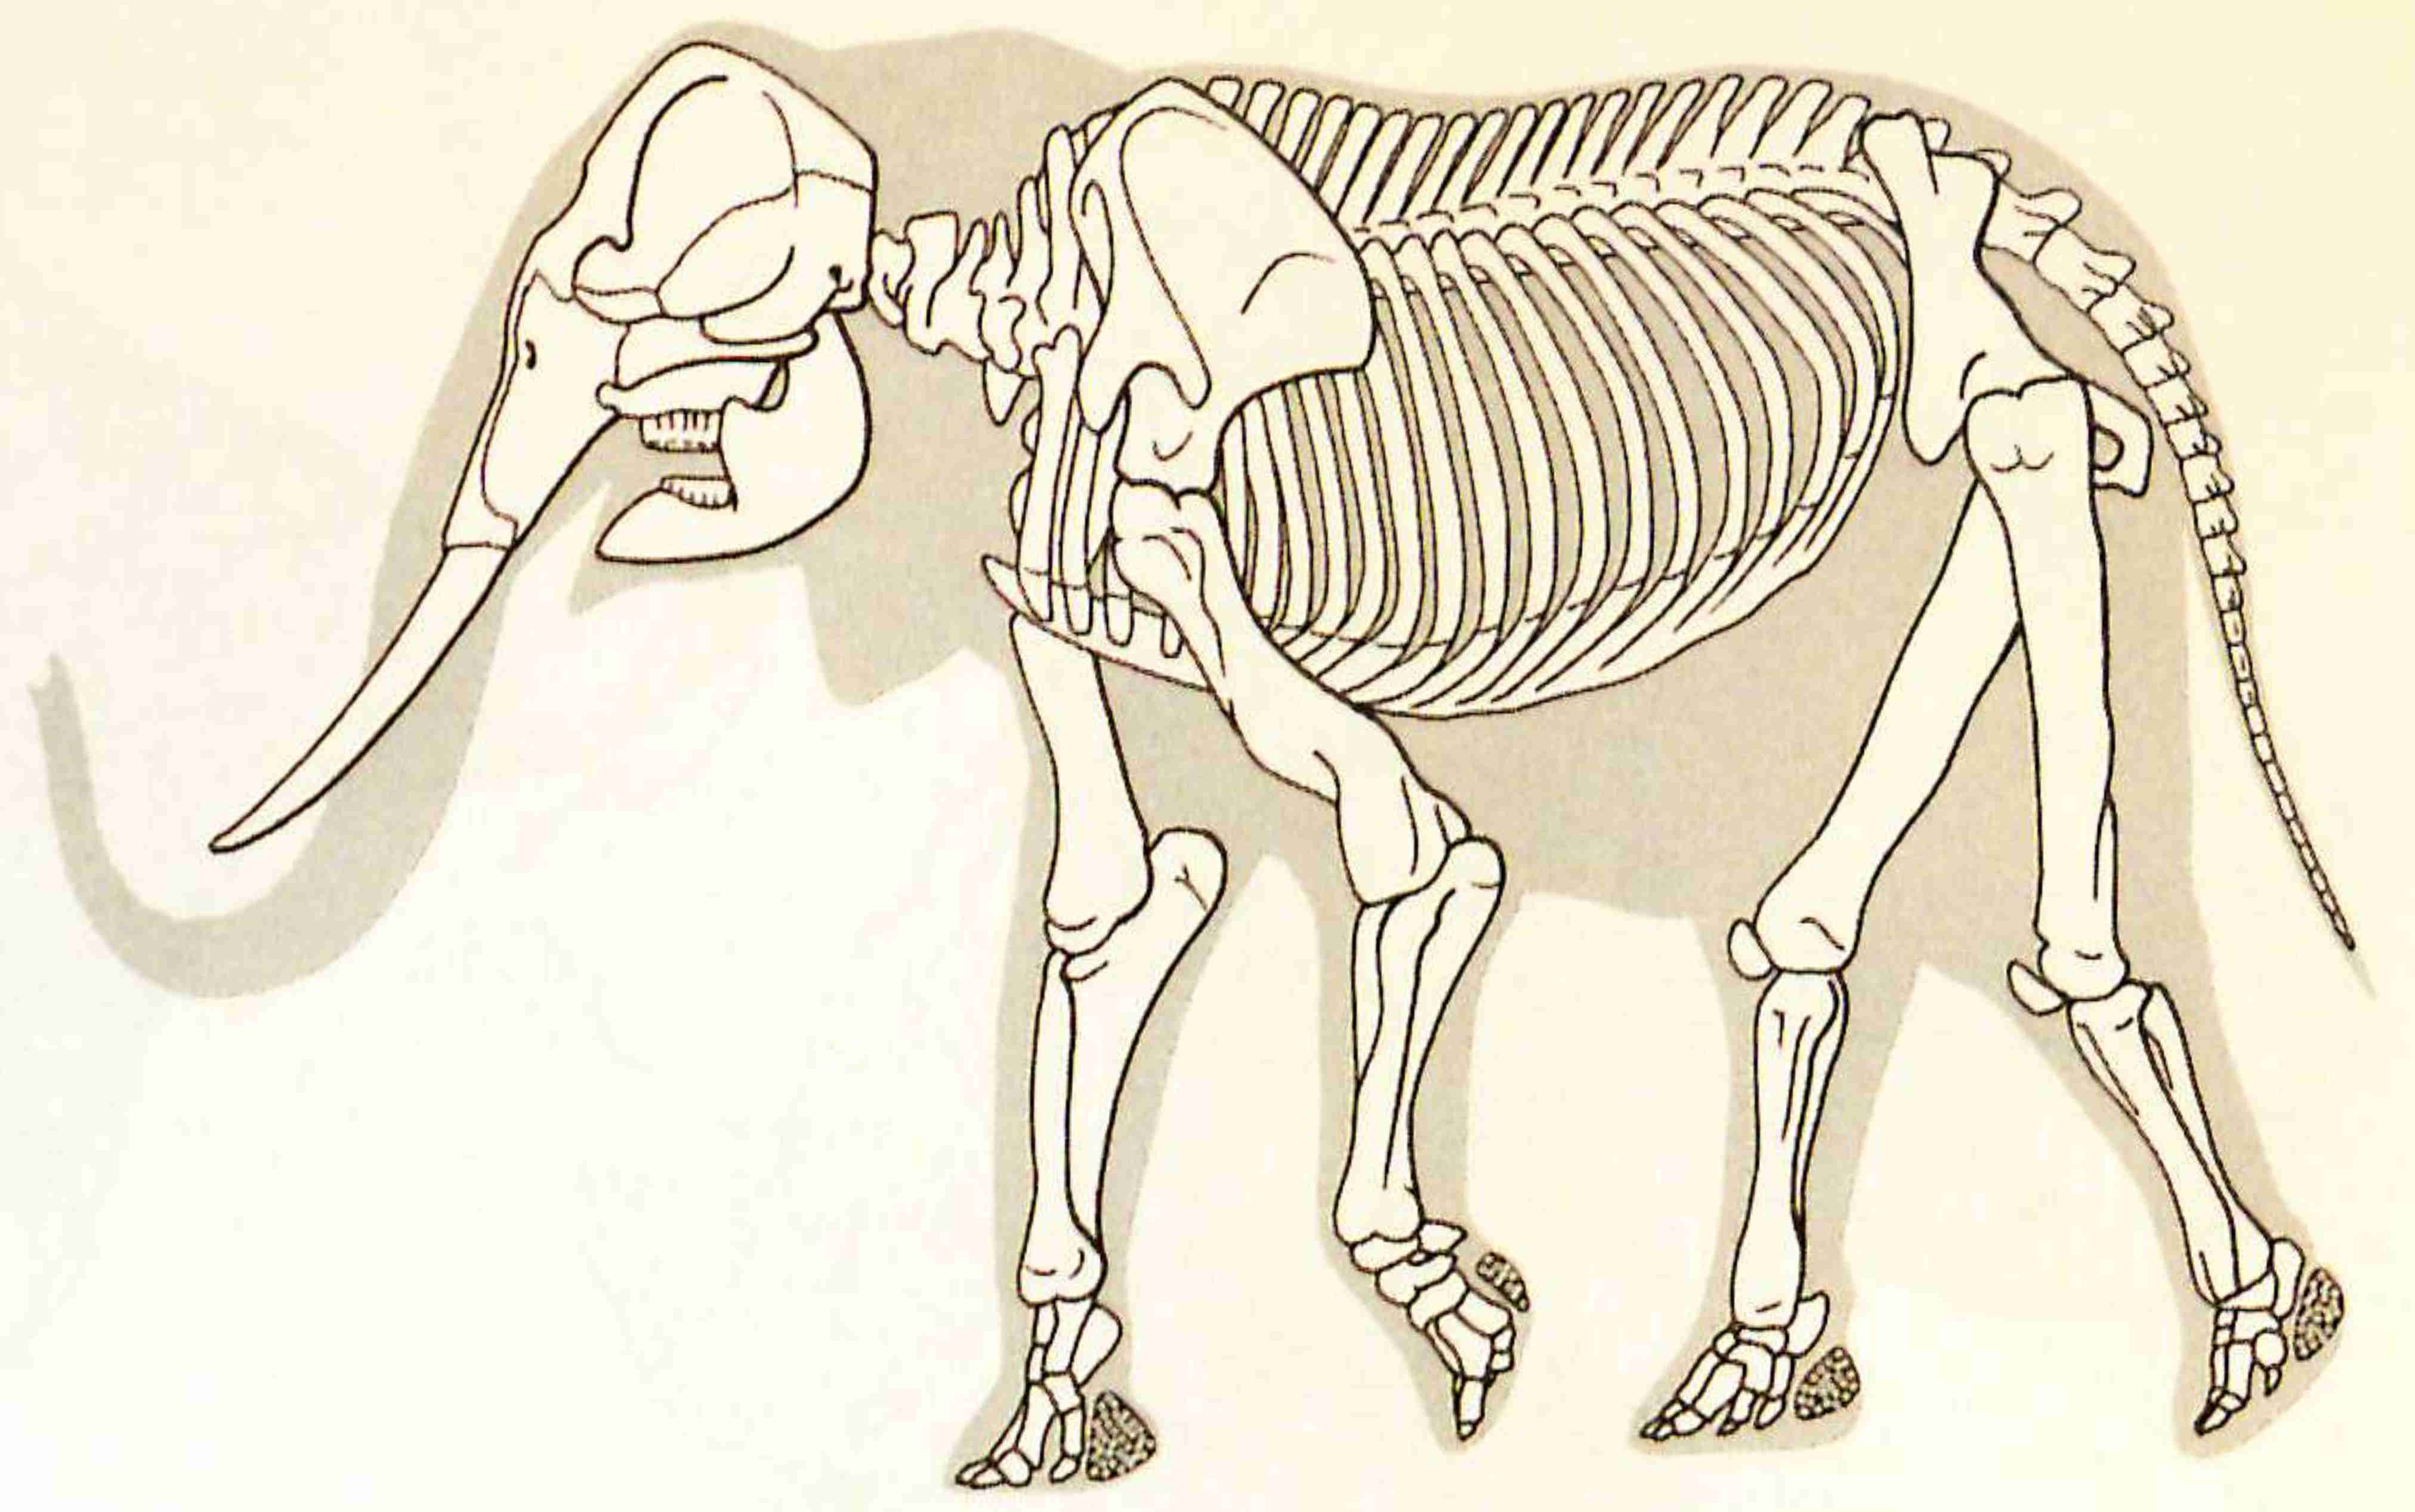
\includegraphics[width=0.2\textwidth]{../PCA/Skelettbilder_klein/Afrikanischer_Elefant.jpg}}~
\subfloat[Amerikanischer Flussbarsch]{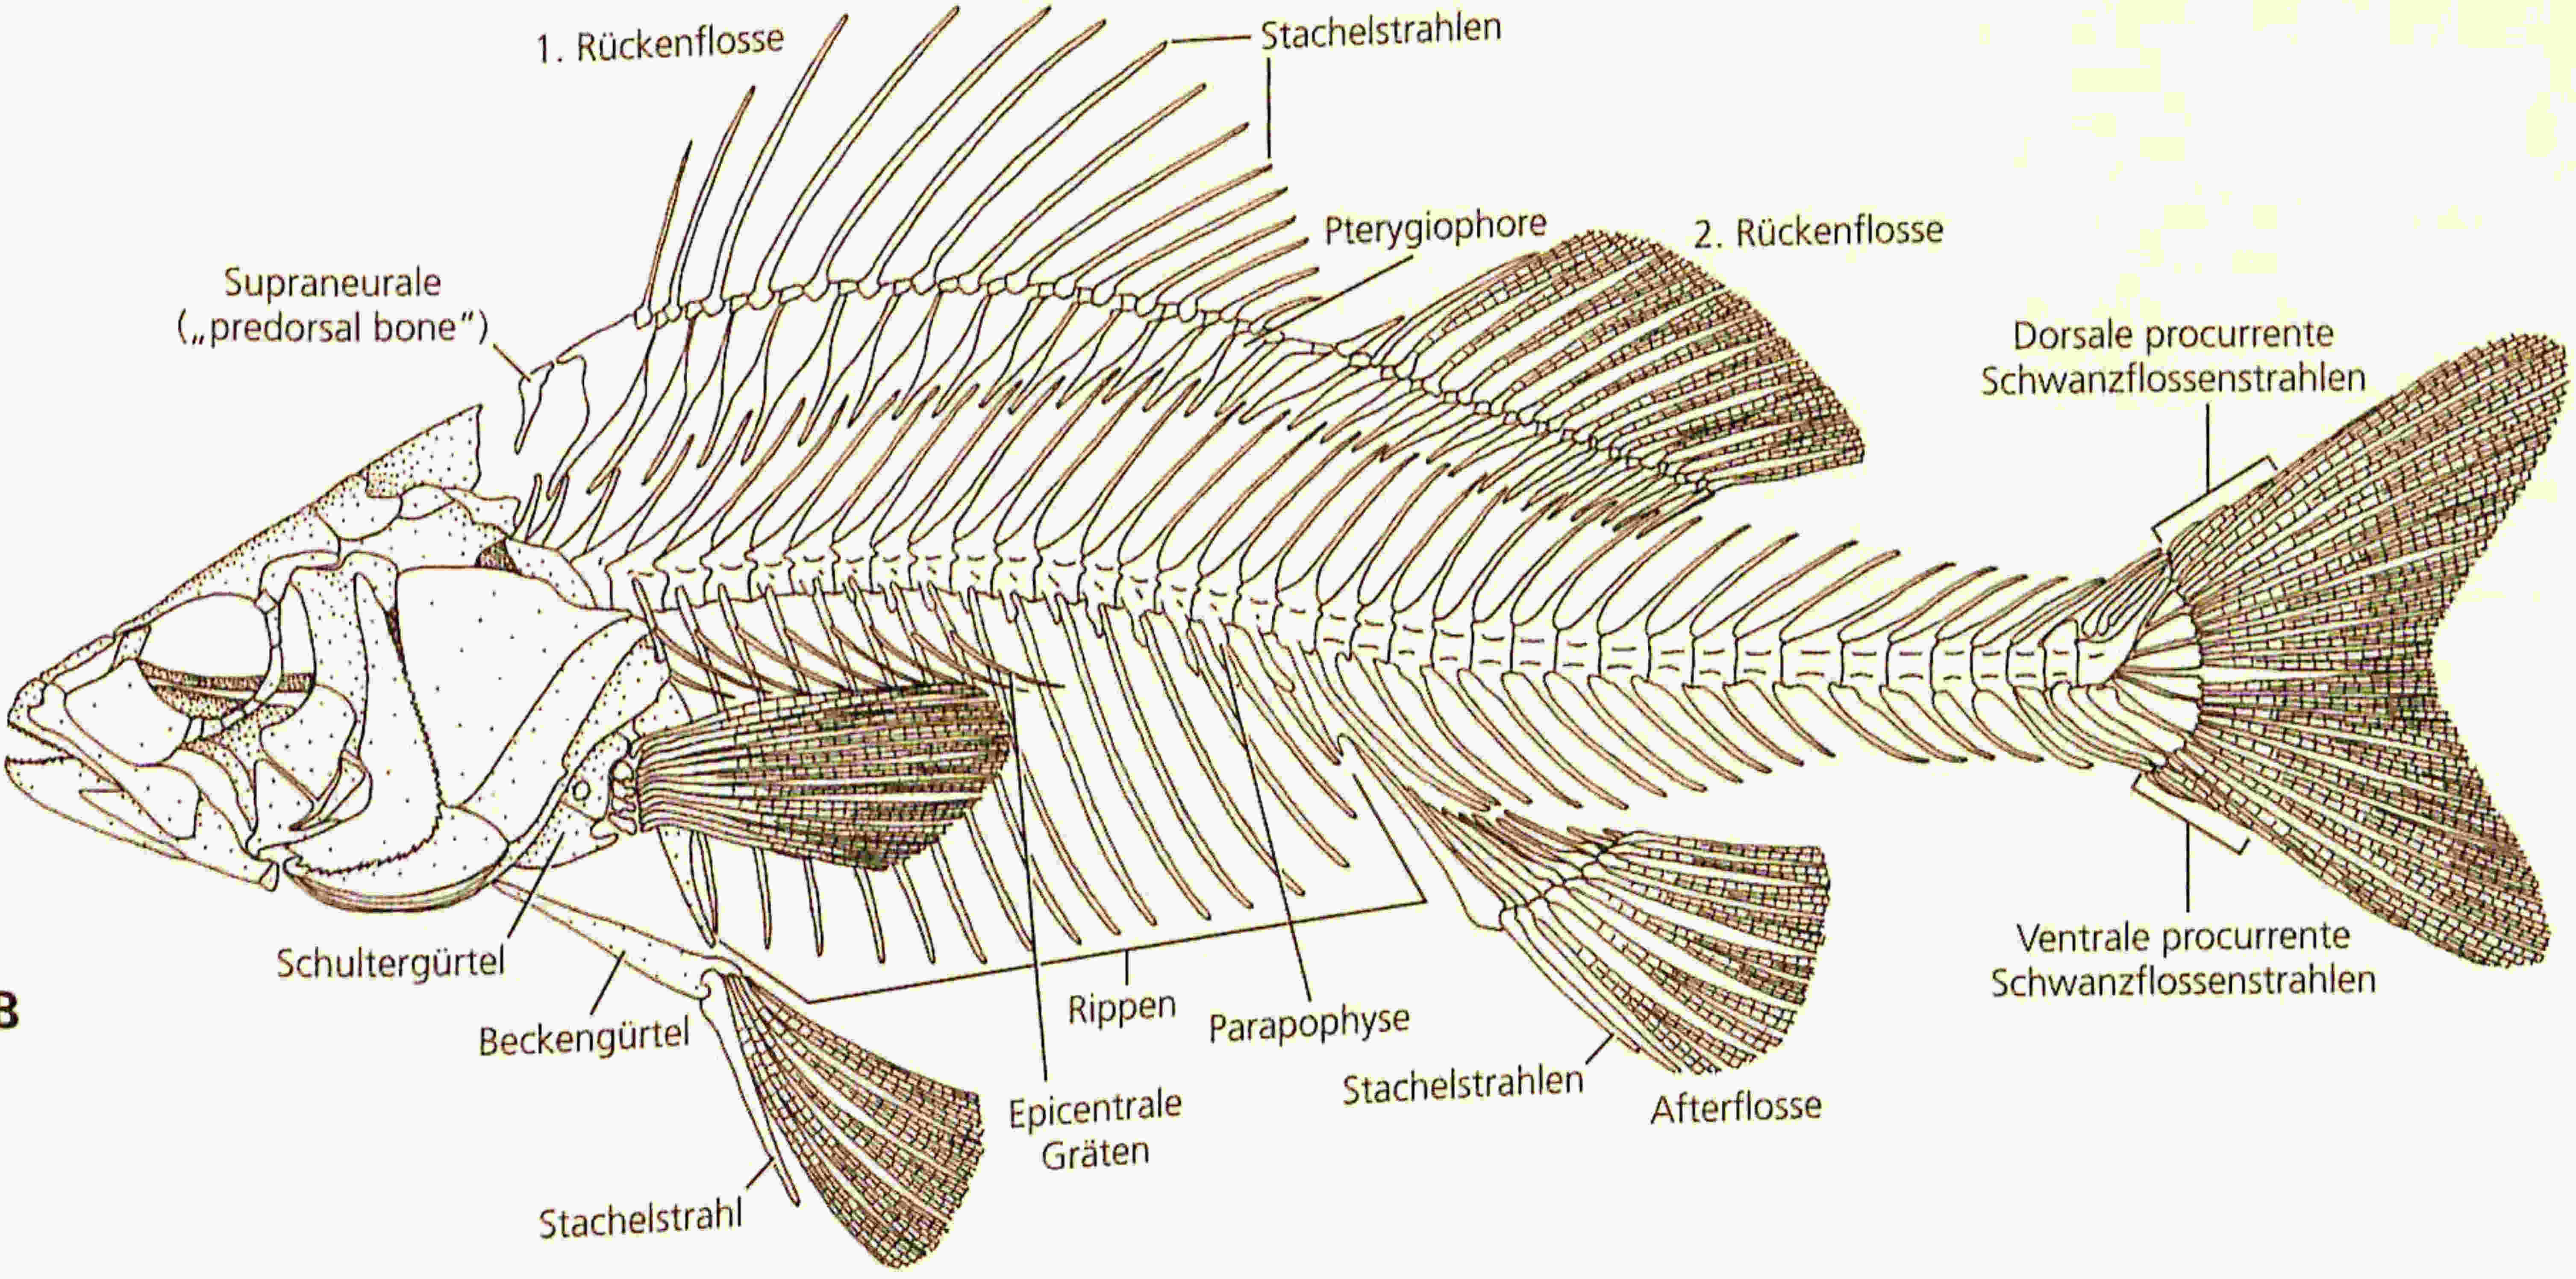
\includegraphics[width=0.2\textwidth]{../PCA/Skelettbilder_klein/Amerikanischer_Flussbarsch.jpg}}~
\subfloat[Archaeopteryx]{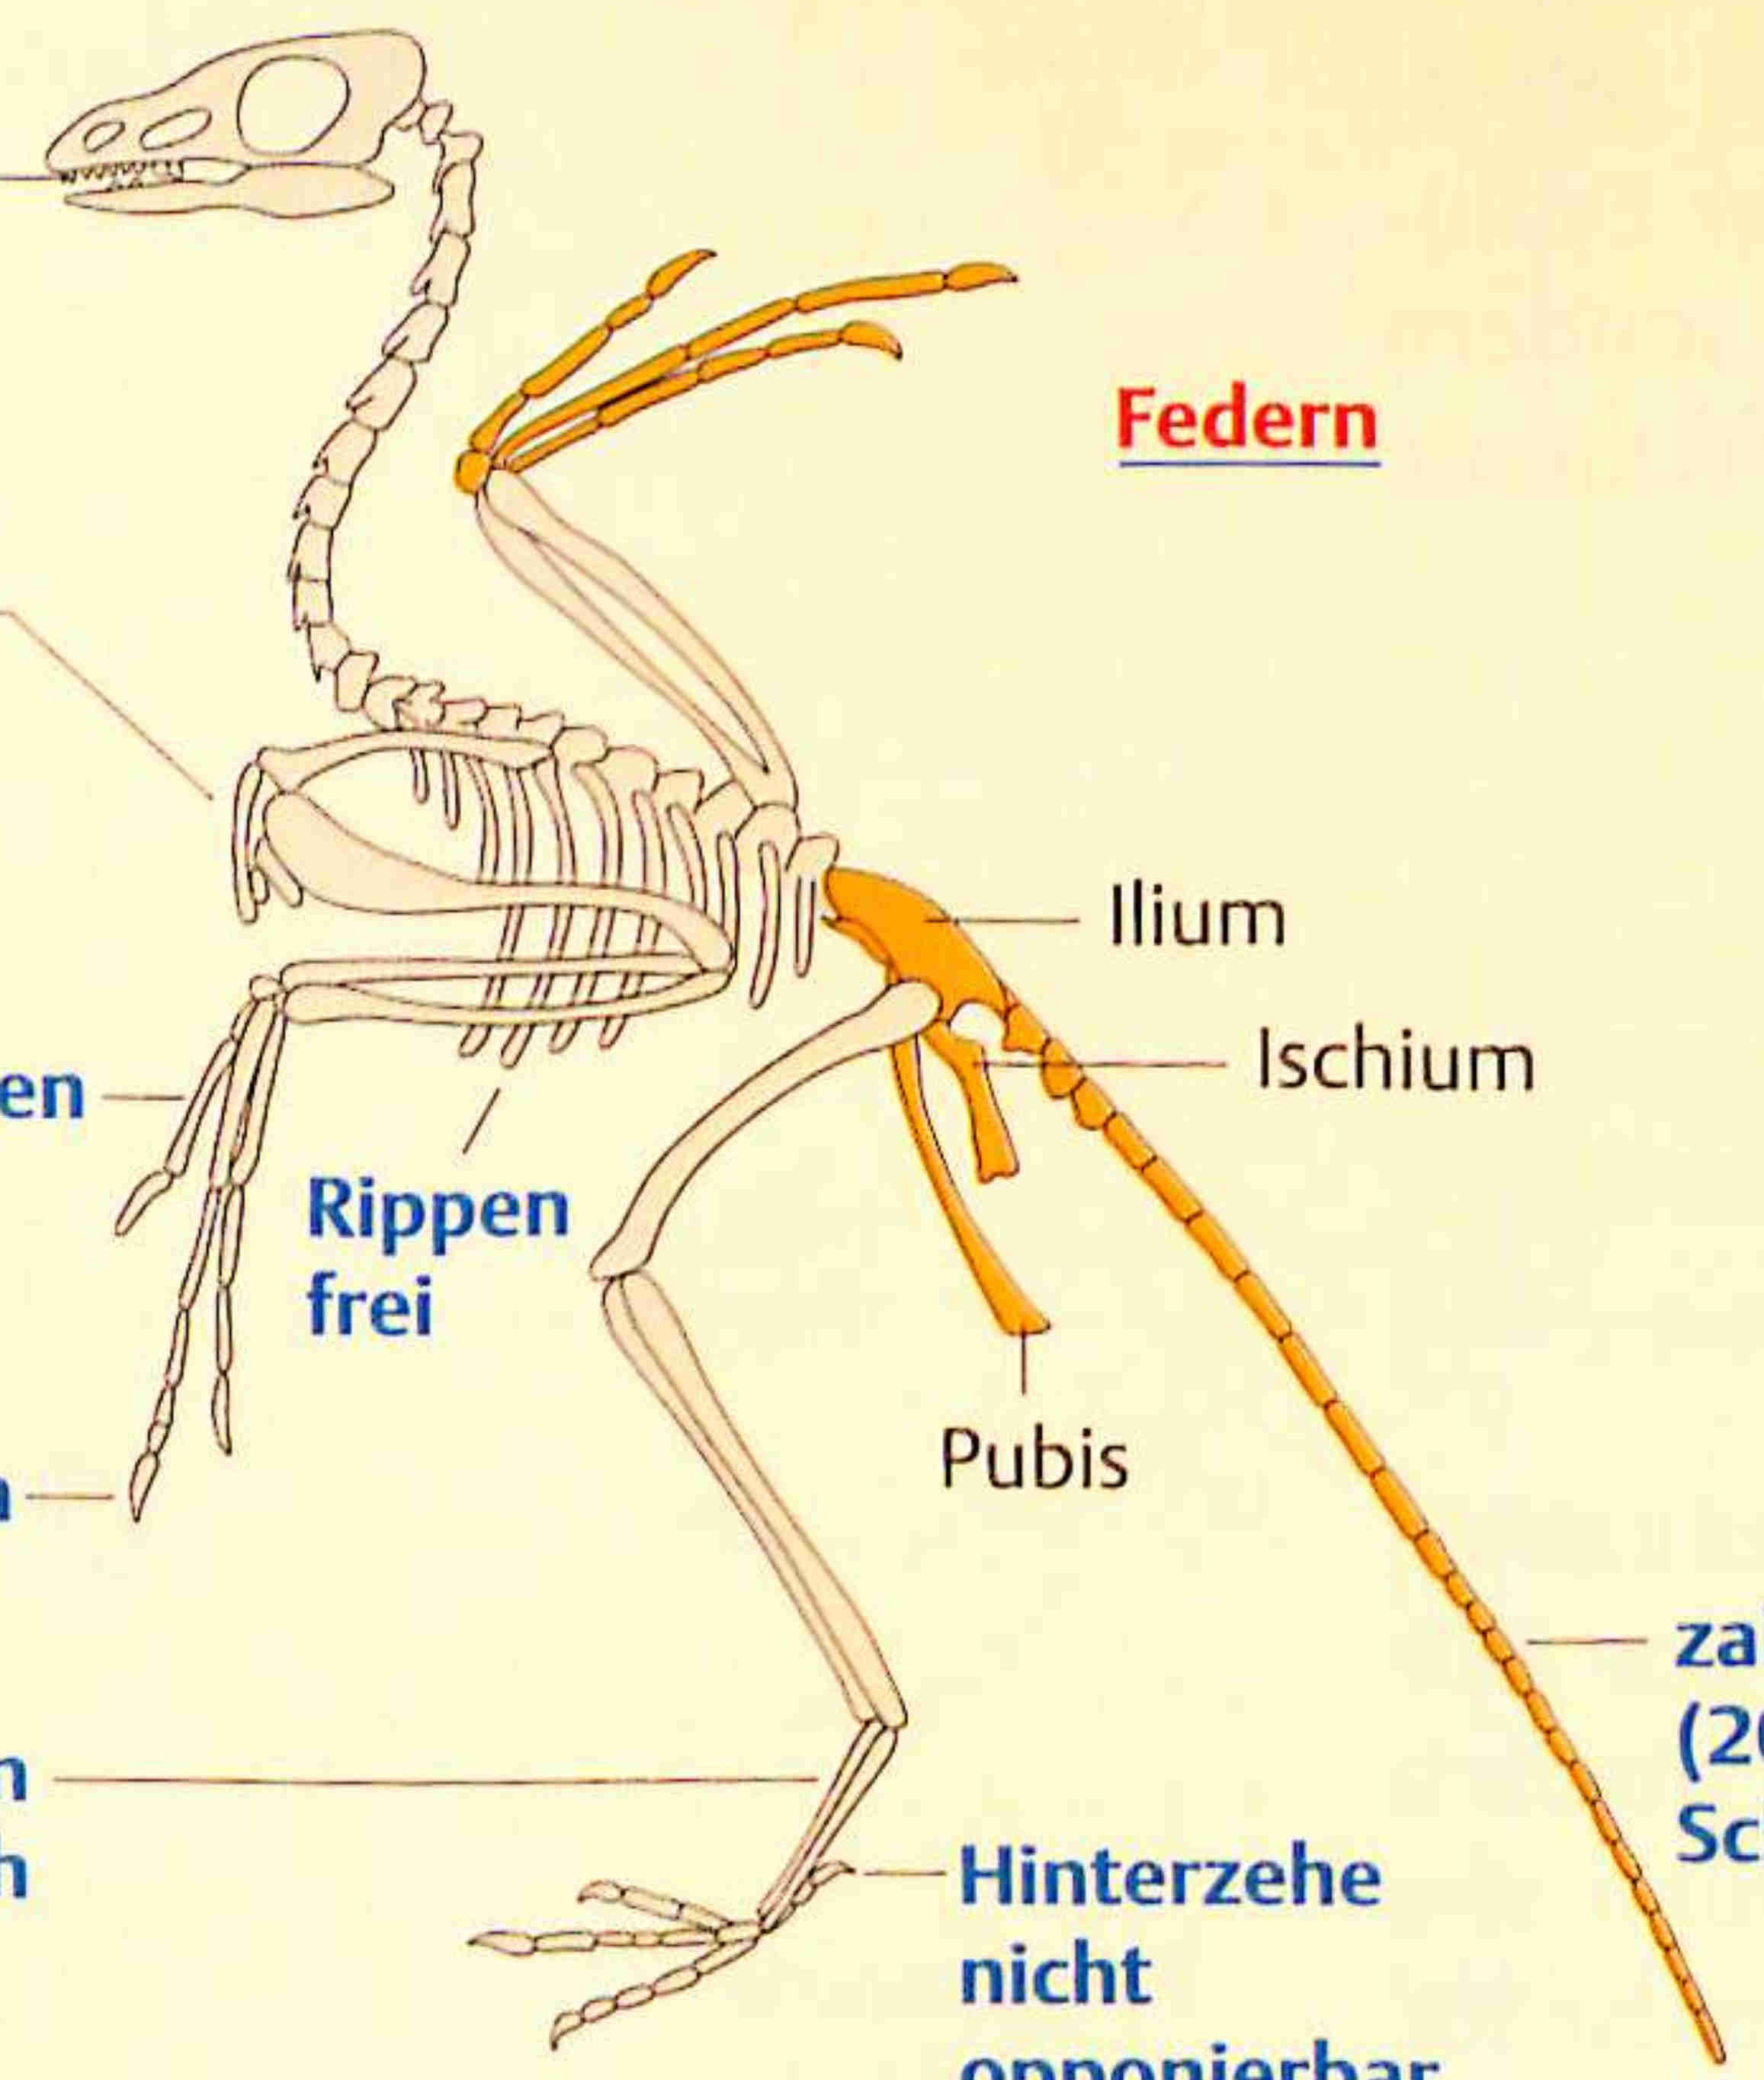
\includegraphics[width=0.2\textwidth]{../PCA/Skelettbilder_klein/Archaeopteryx.jpg}}~
\subfloat[Blauwal]{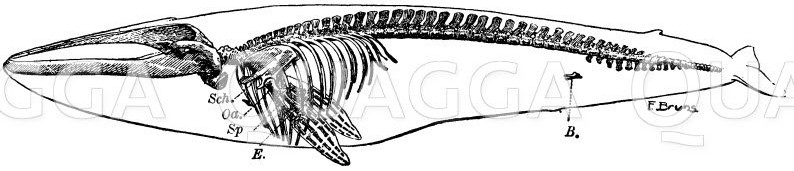
\includegraphics[width=0.2\textwidth]{../PCA/Skelettbilder_klein/Blauwal.jpg}}~
\subfloat[Brachiosaurus]{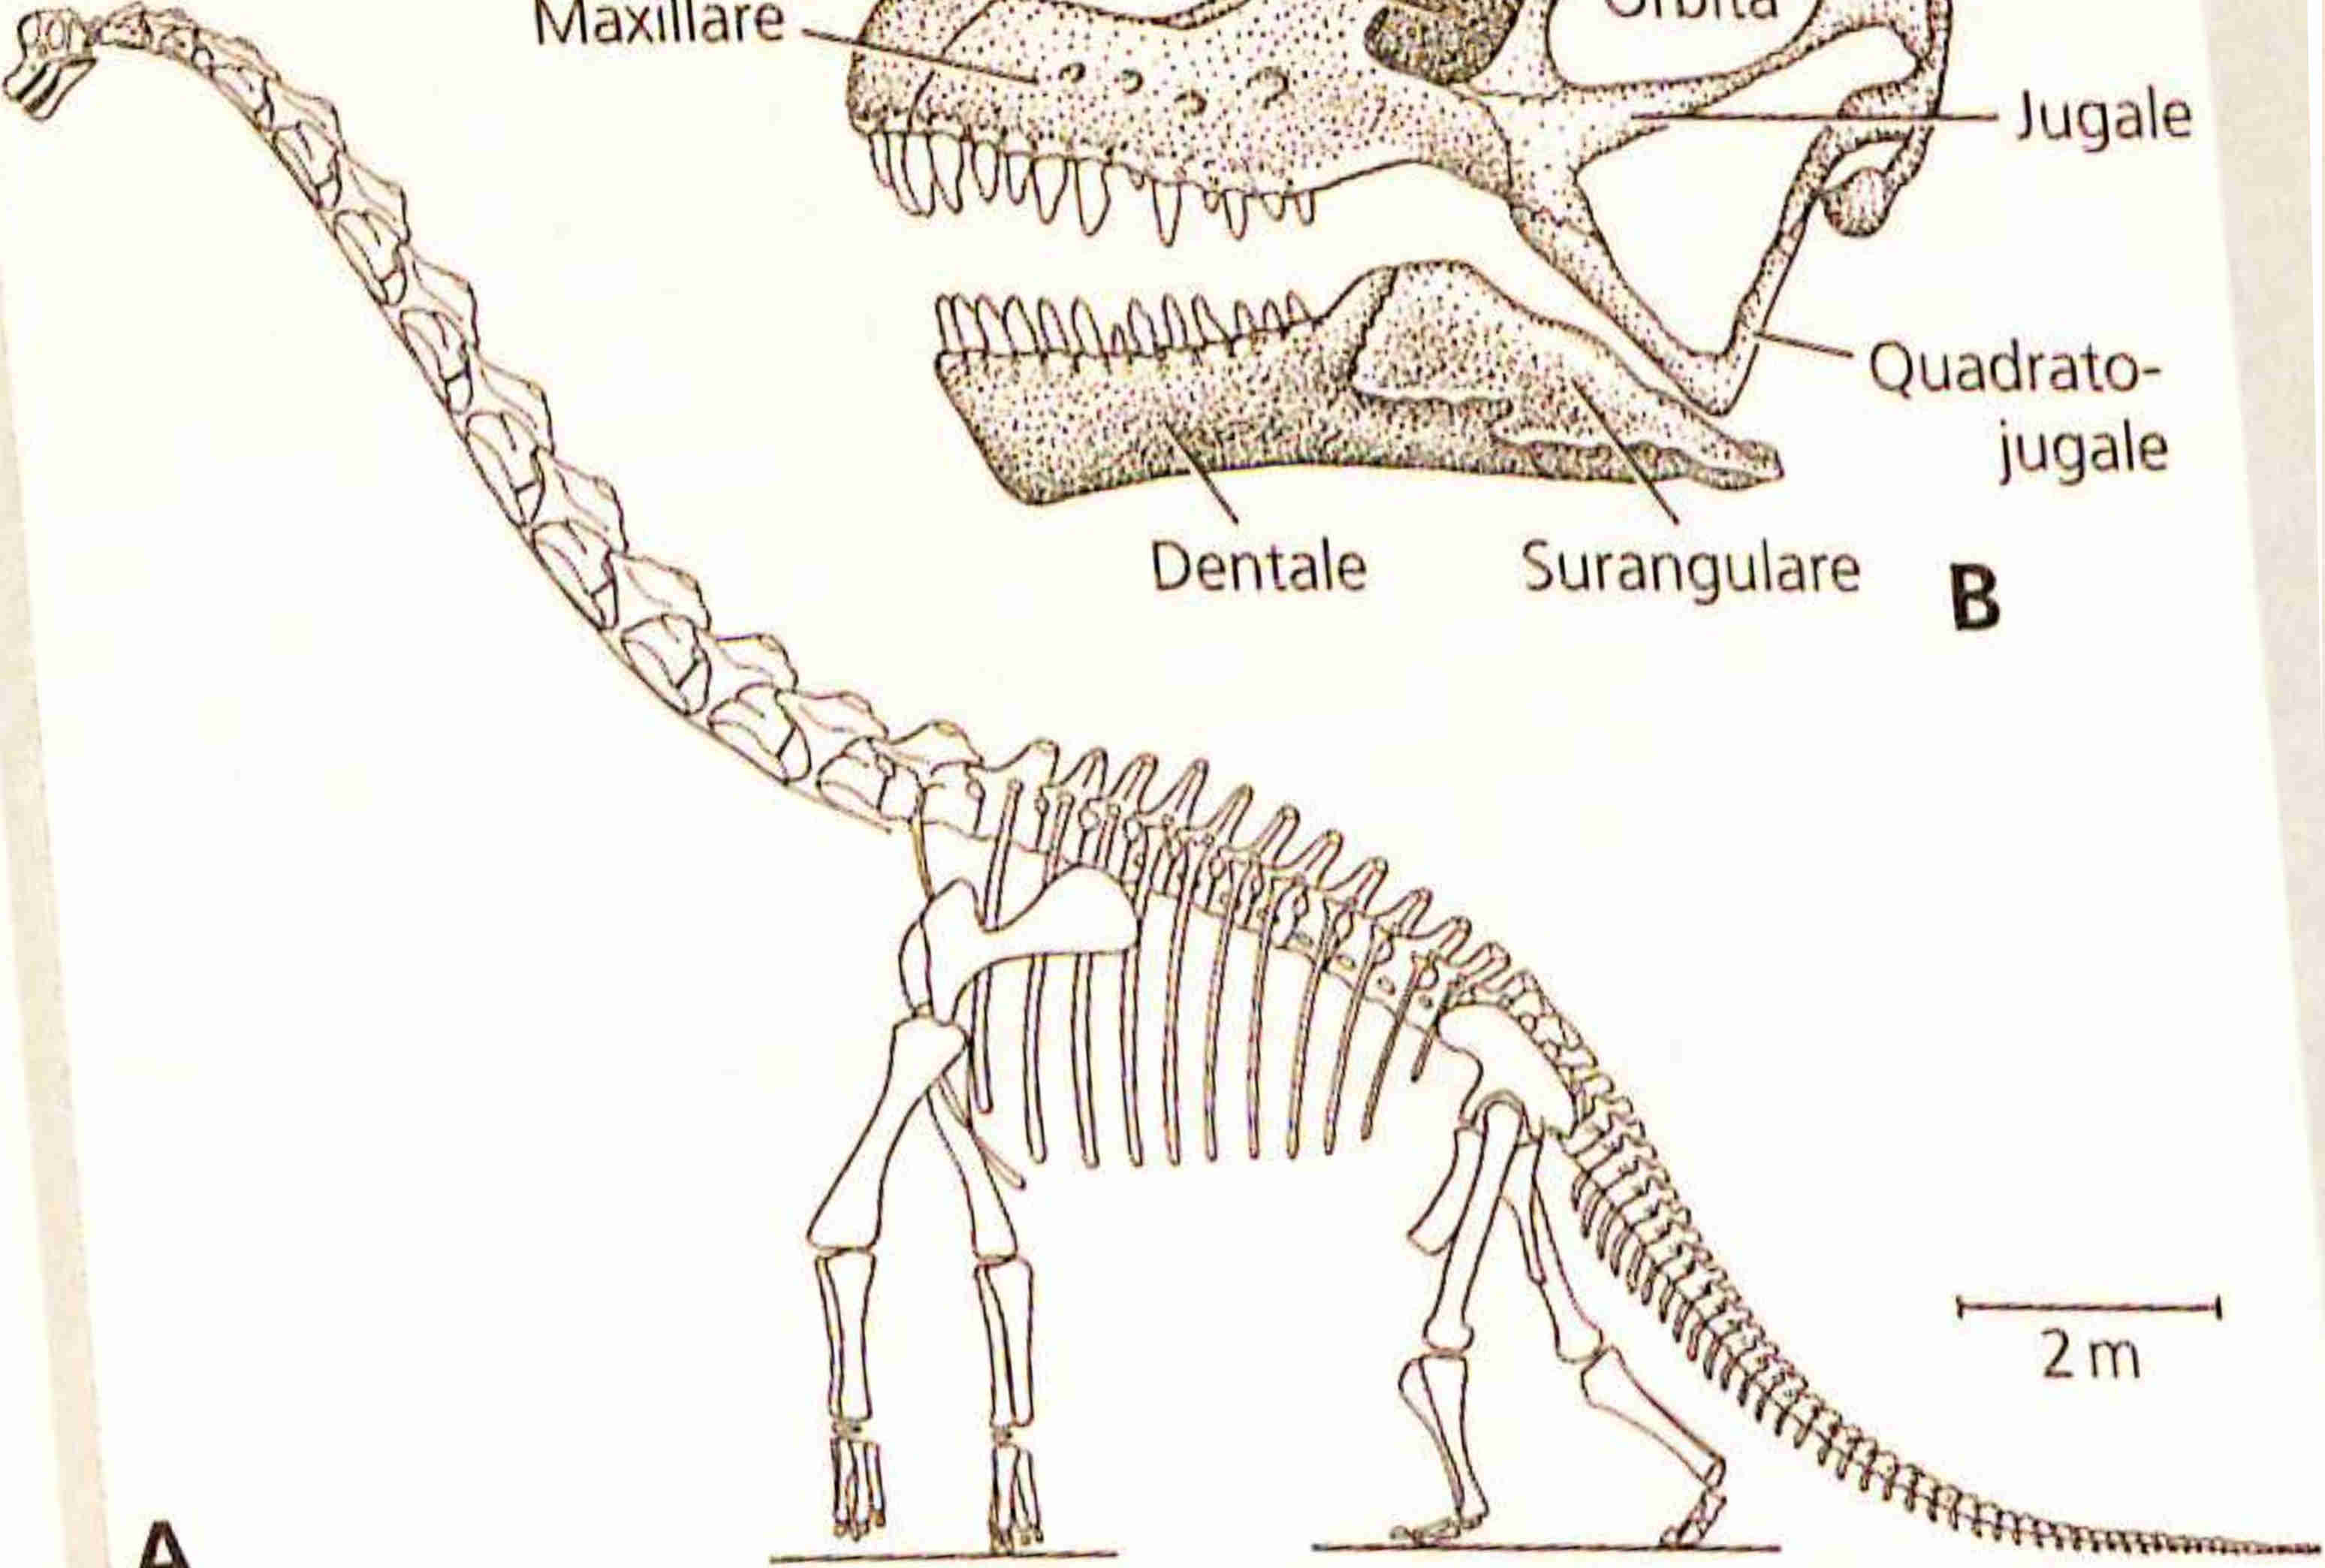
\includegraphics[width=0.2\textwidth]{../PCA/Skelettbilder_klein/Brachiosaurus.jpg}}
\\
\subfloat[Chamäleon]{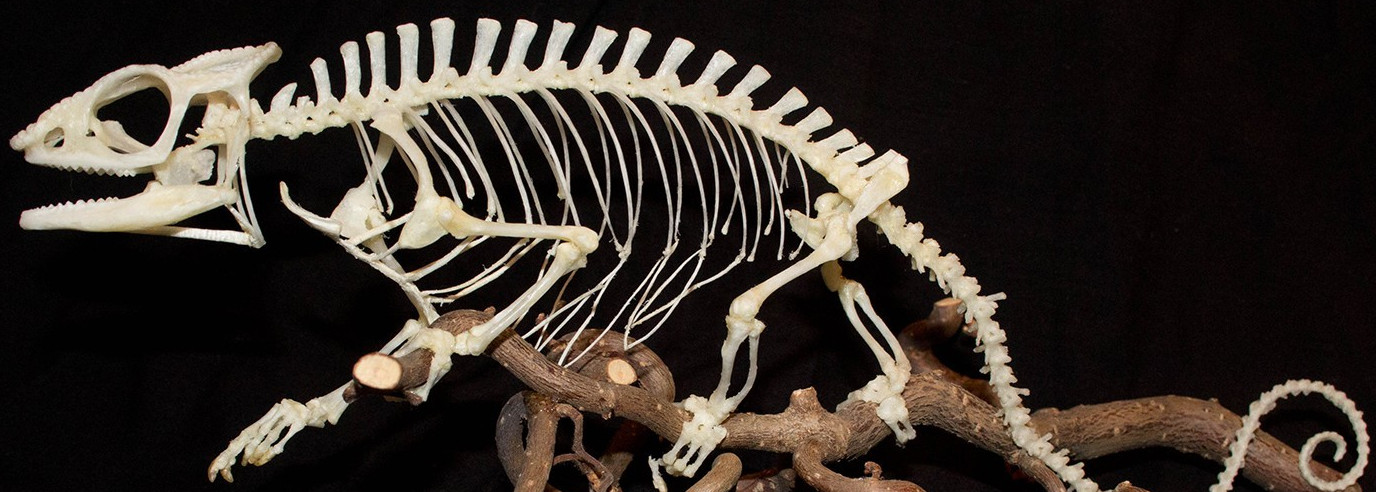
\includegraphics[width=0.2\textwidth]{../PCA/Skelettbilder_klein/Chamaeleon.jpg}}~
\subfloat[Dimetrodon]{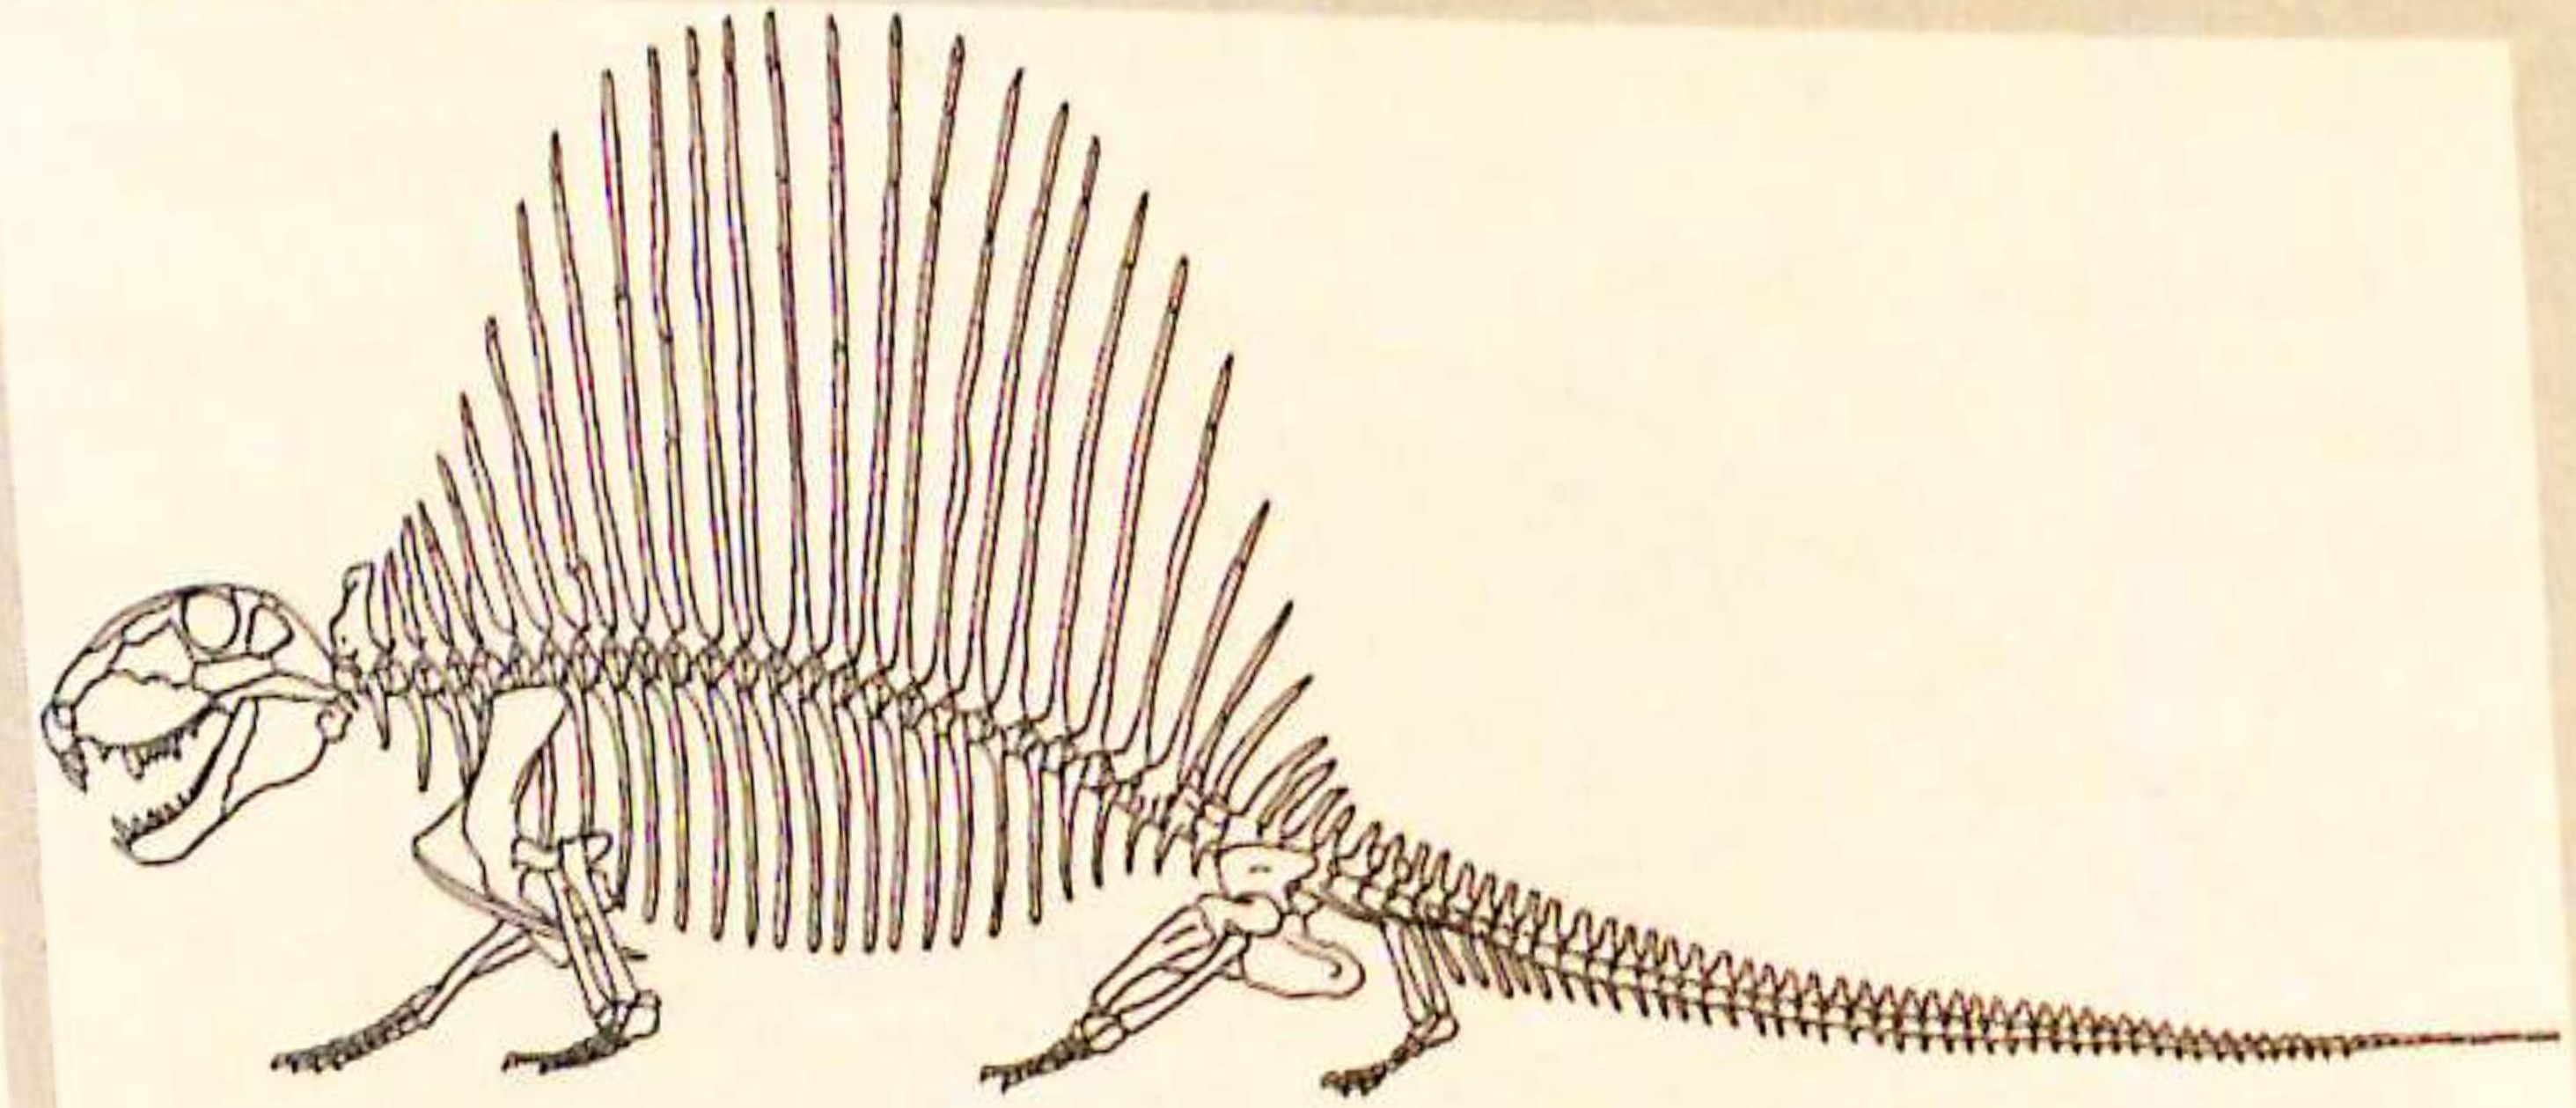
\includegraphics[width=0.2\textwidth]{../PCA/Skelettbilder_klein/Dimetrodon.jpg}}~
\subfloat[Dromedar]{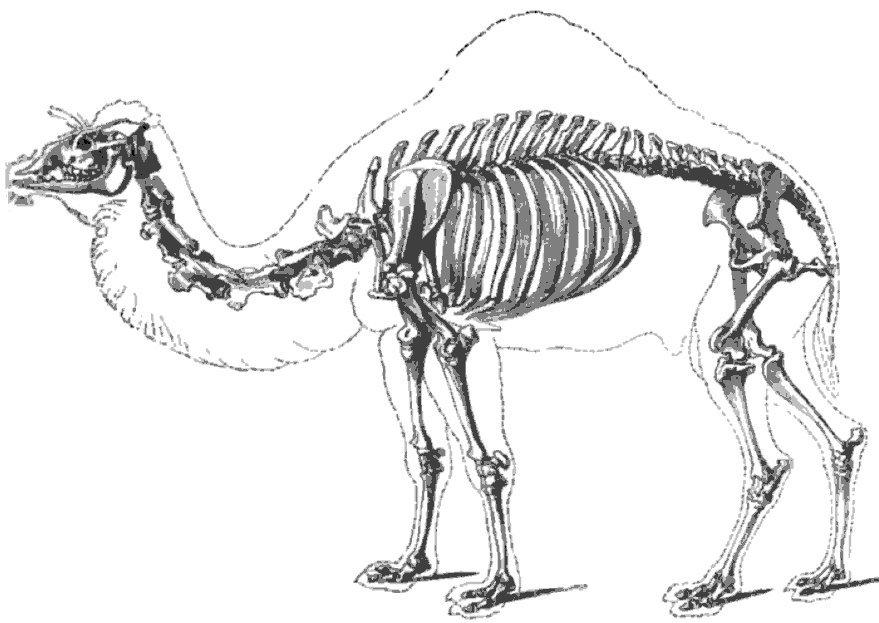
\includegraphics[width=0.2\textwidth]{../PCA/Skelettbilder_klein/Dromedar.jpg}}~
\subfloat[Elster]{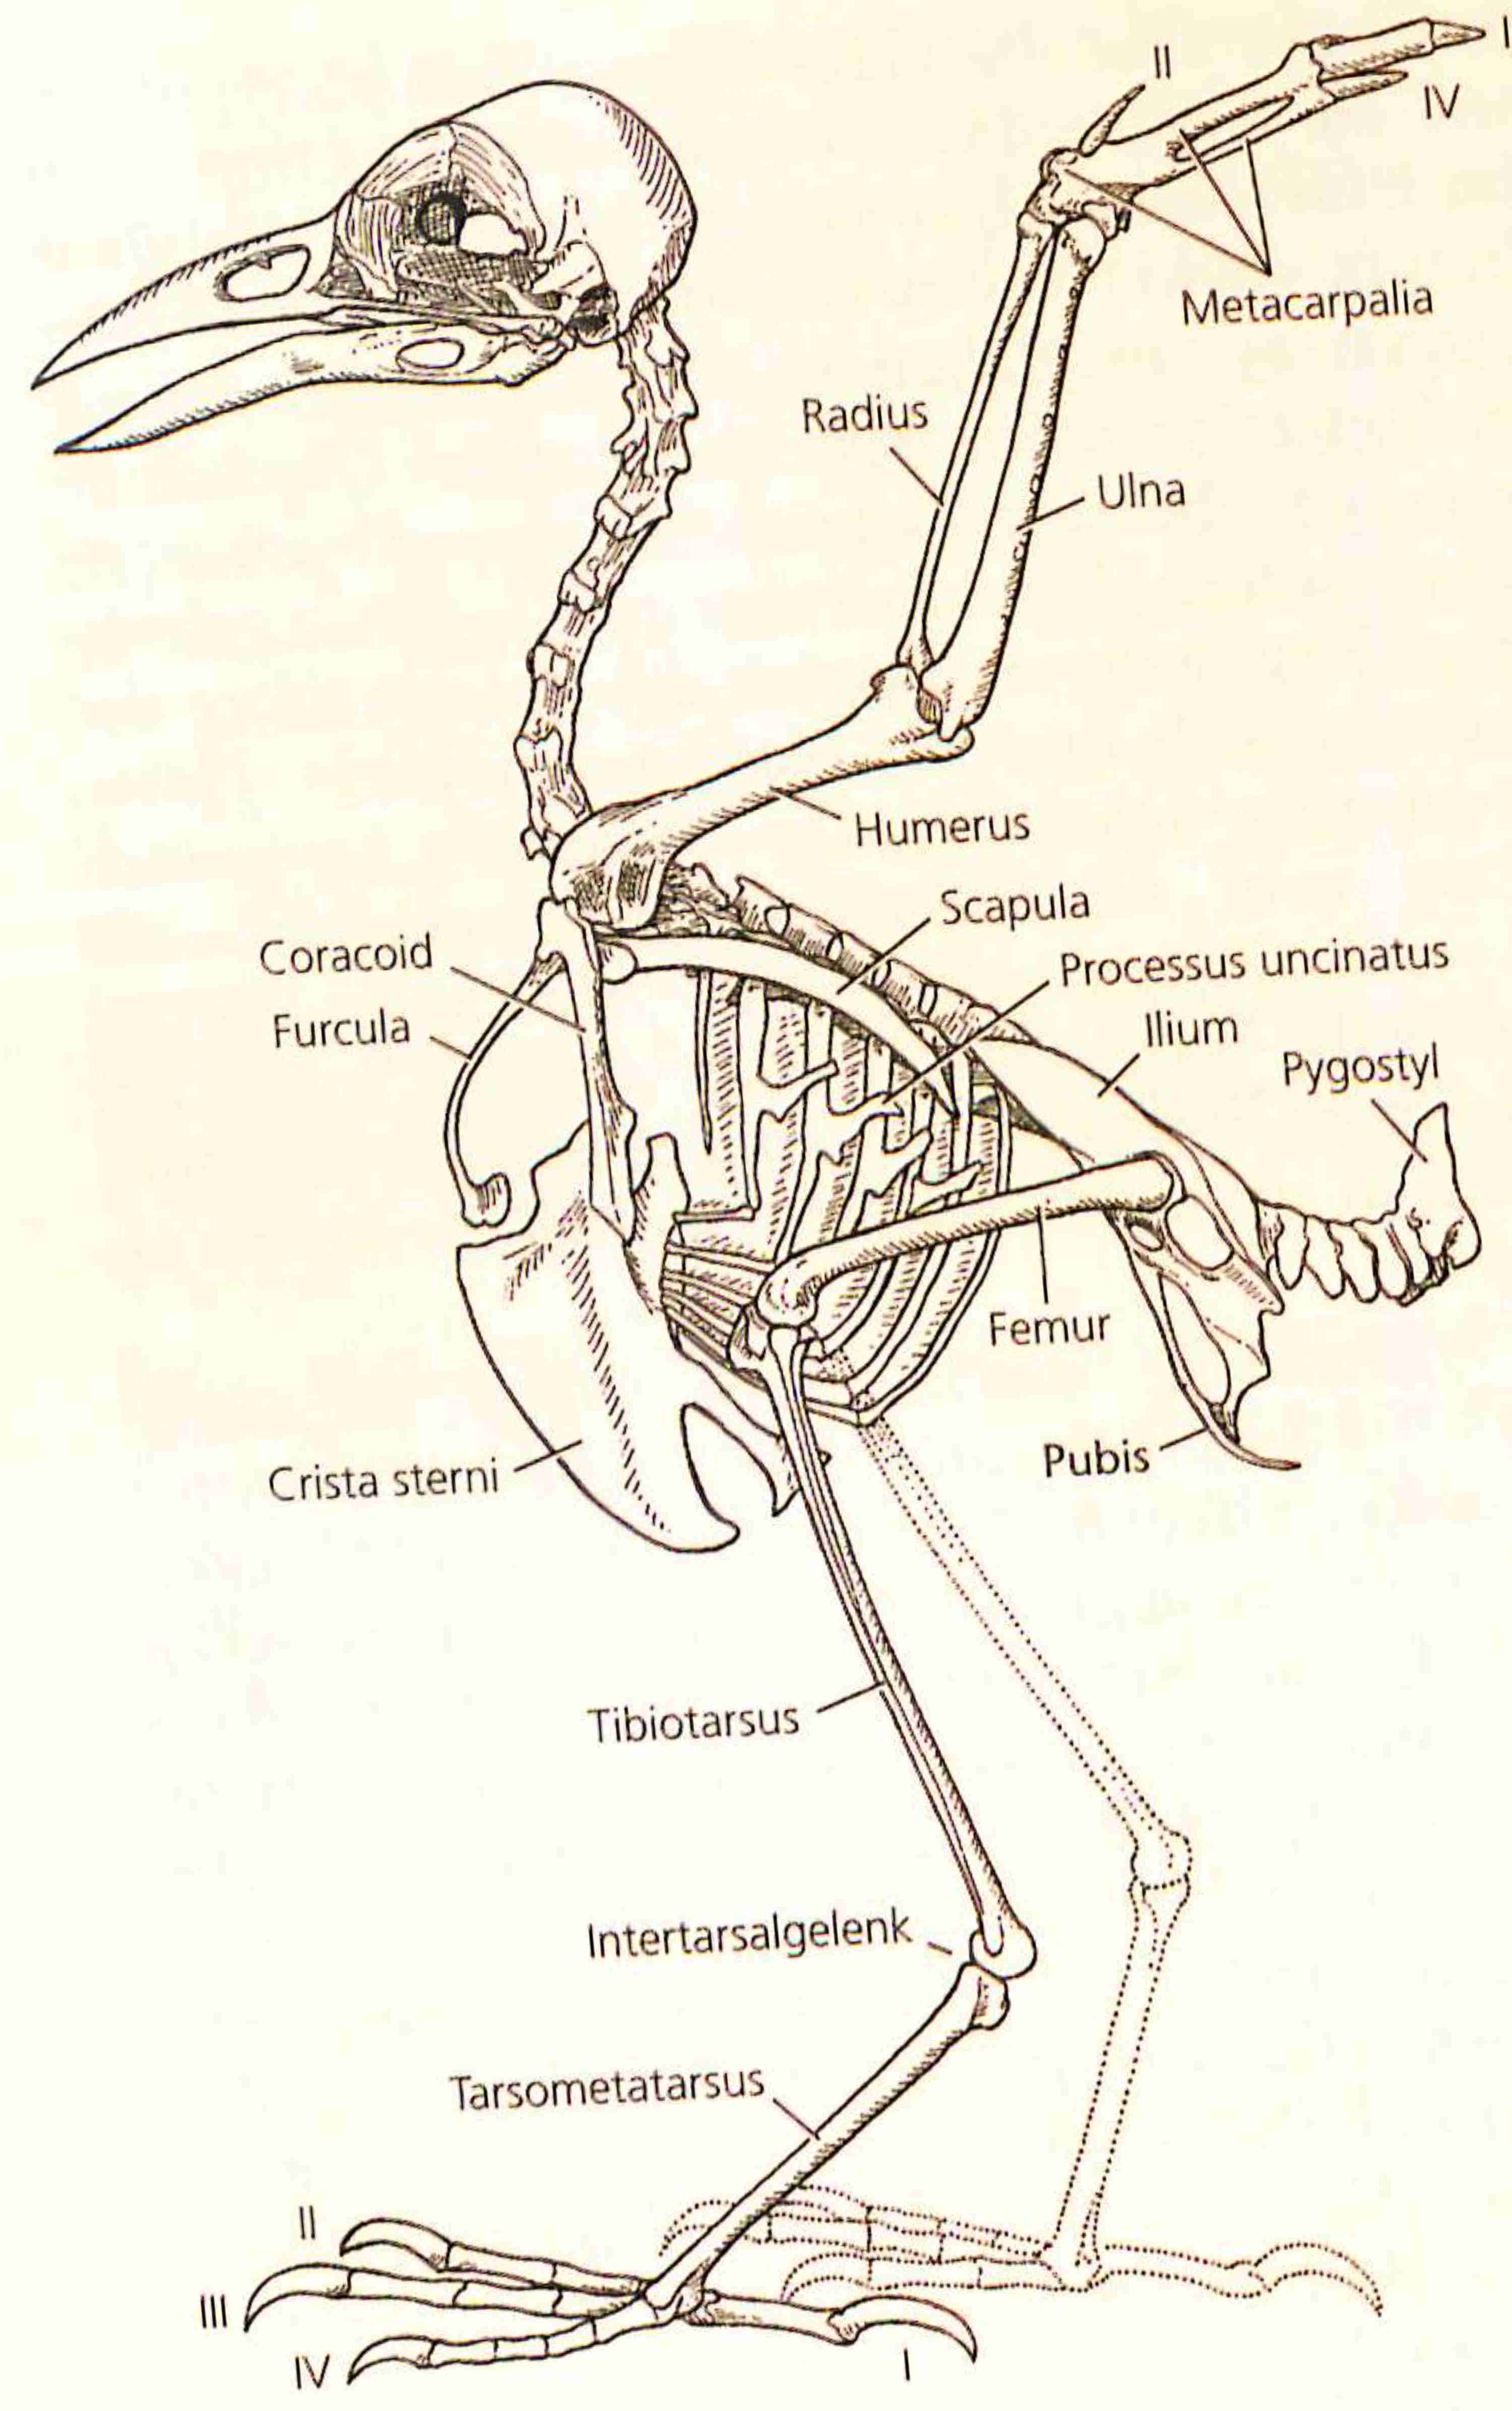
\includegraphics[width=0.2\textwidth]{../PCA/Skelettbilder_klein/Elster.jpg}}~
\subfloat[Forelle]{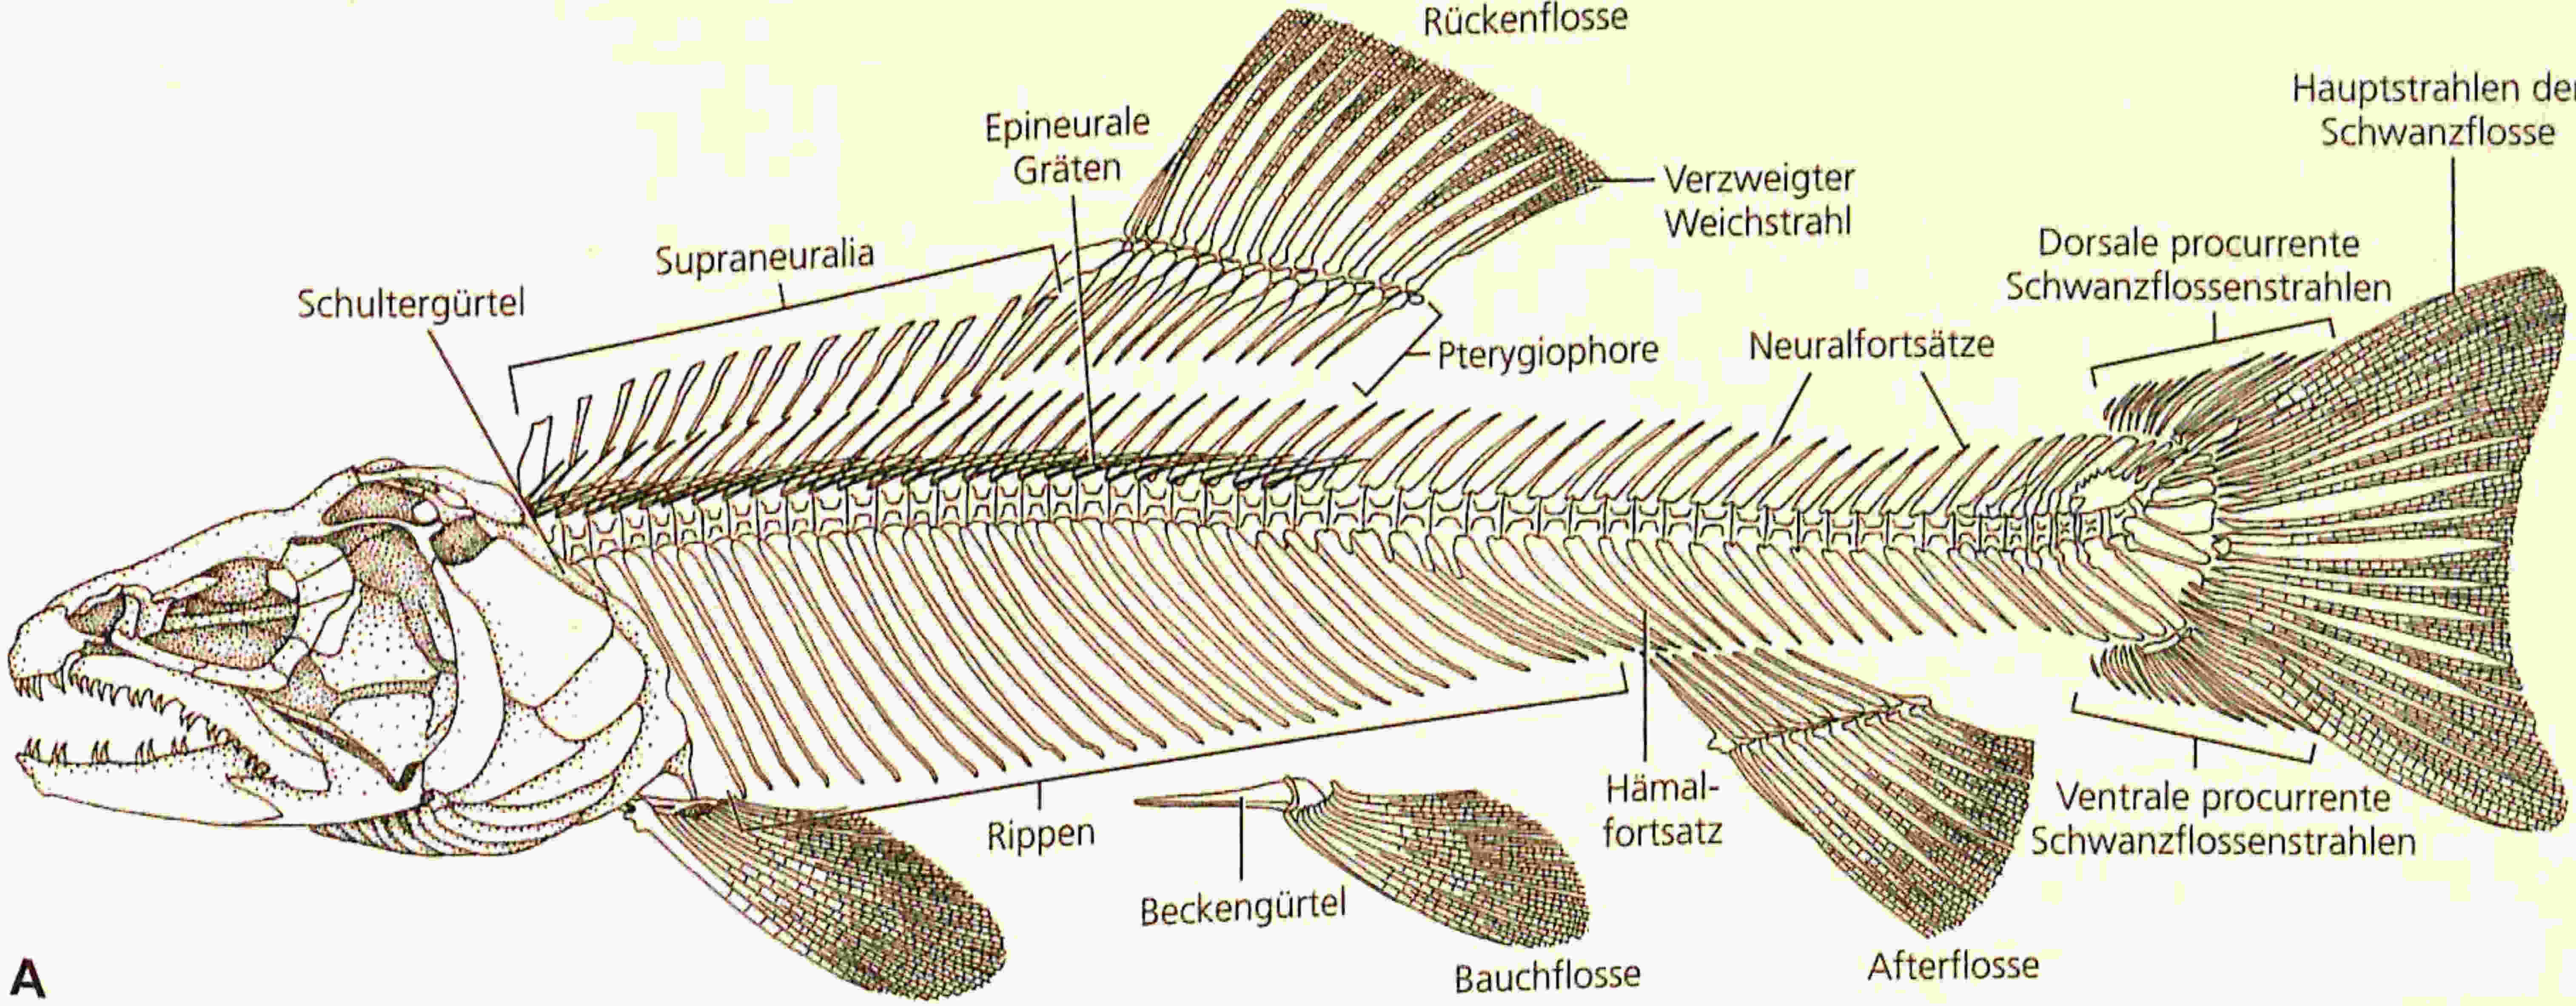
\includegraphics[width=0.2\textwidth]{../PCA/Skelettbilder_klein/Forelle.jpg}}
\\
\subfloat[Frosch]{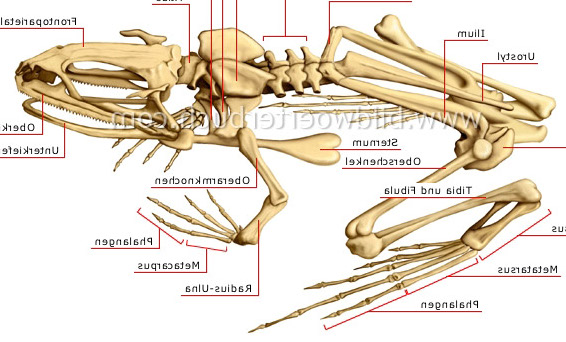
\includegraphics[width=0.2\textwidth]{../PCA/Skelettbilder_klein/Frosch.jpg}}~
\subfloat[Gämse]{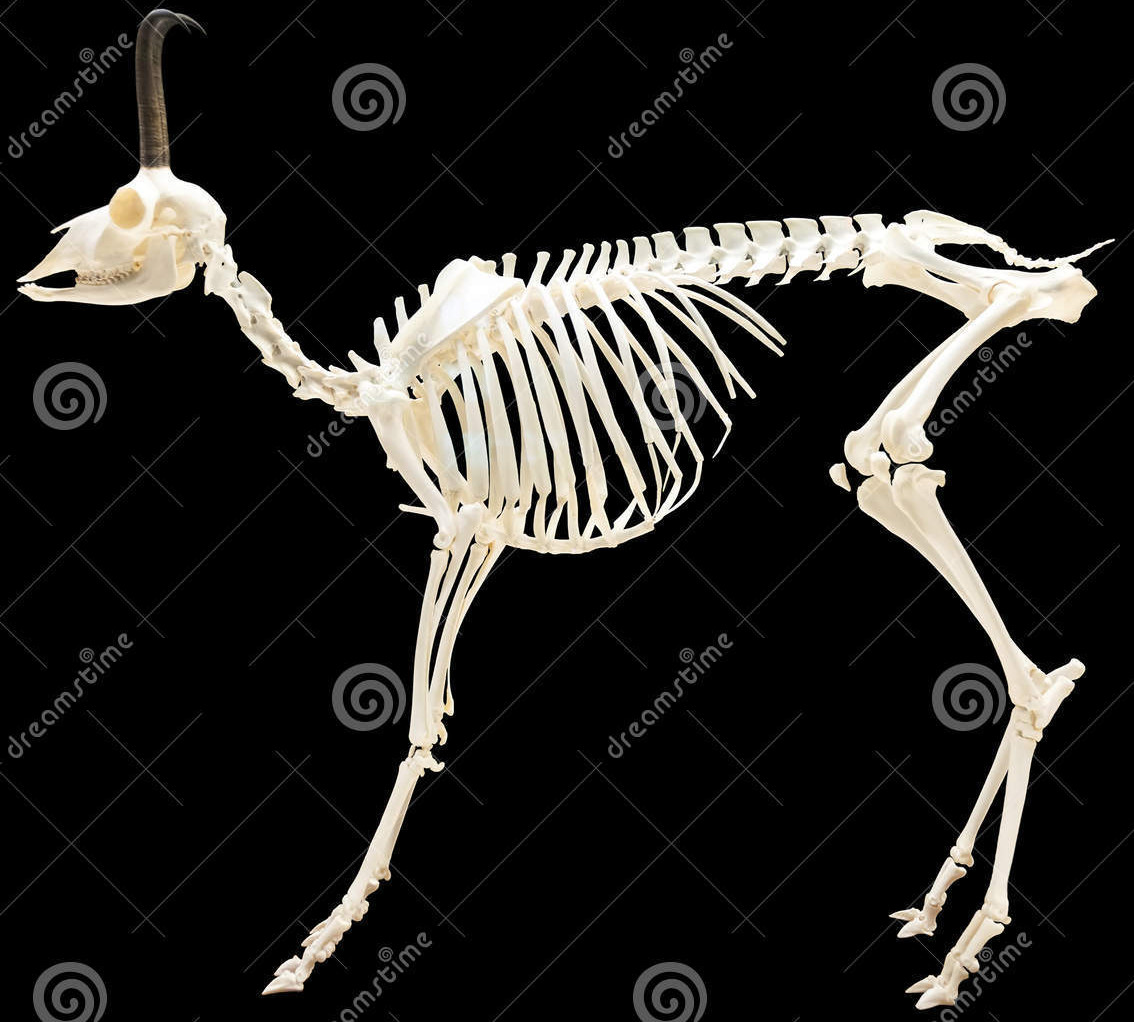
\includegraphics[width=0.2\textwidth]{../PCA/Skelettbilder_klein/Gaemse.jpg}}~
\subfloat[Giraffe]{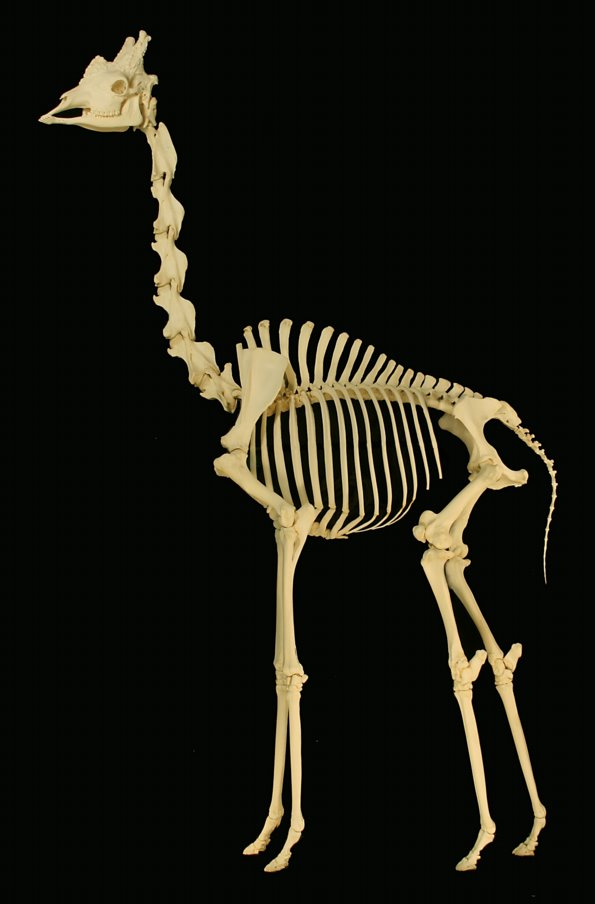
\includegraphics[width=0.2\textwidth]{../PCA/Skelettbilder_klein/Giraffe.jpg}}~
\subfloat[Gnu]{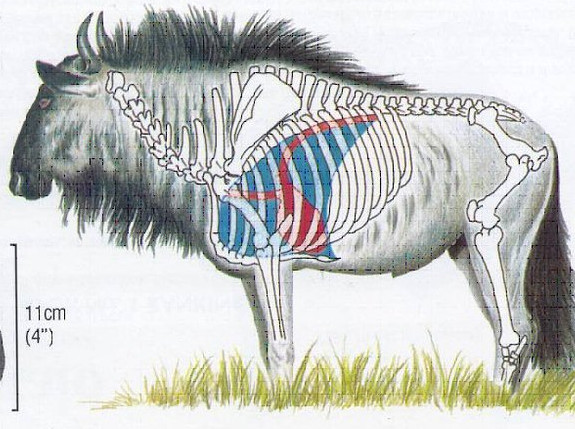
\includegraphics[width=0.2\textwidth]{../PCA/Skelettbilder_klein/Gnu.jpg}}~
\subfloat[Grönlandwal]{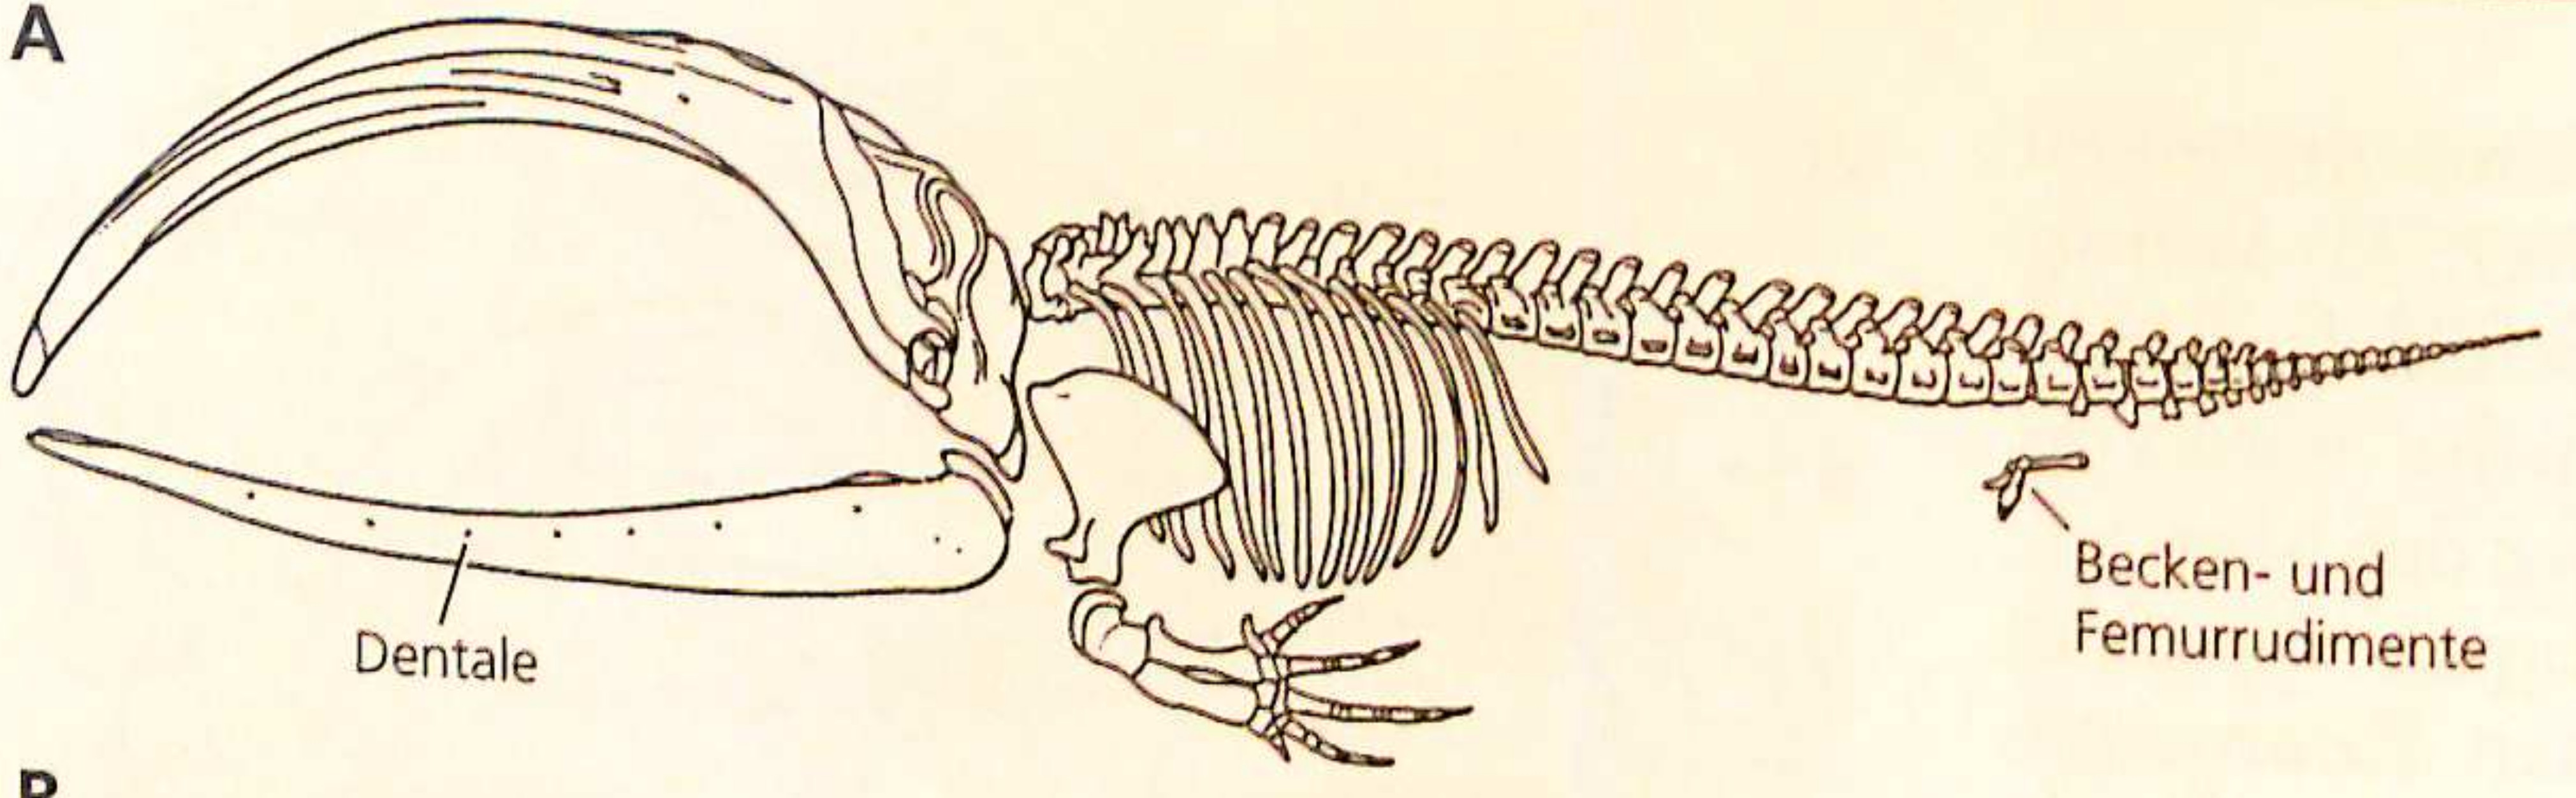
\includegraphics[width=0.2\textwidth]{../PCA/Skelettbilder_klein/Groenlandwal.jpg}}
\\
\subfloat[Ichthyornis]{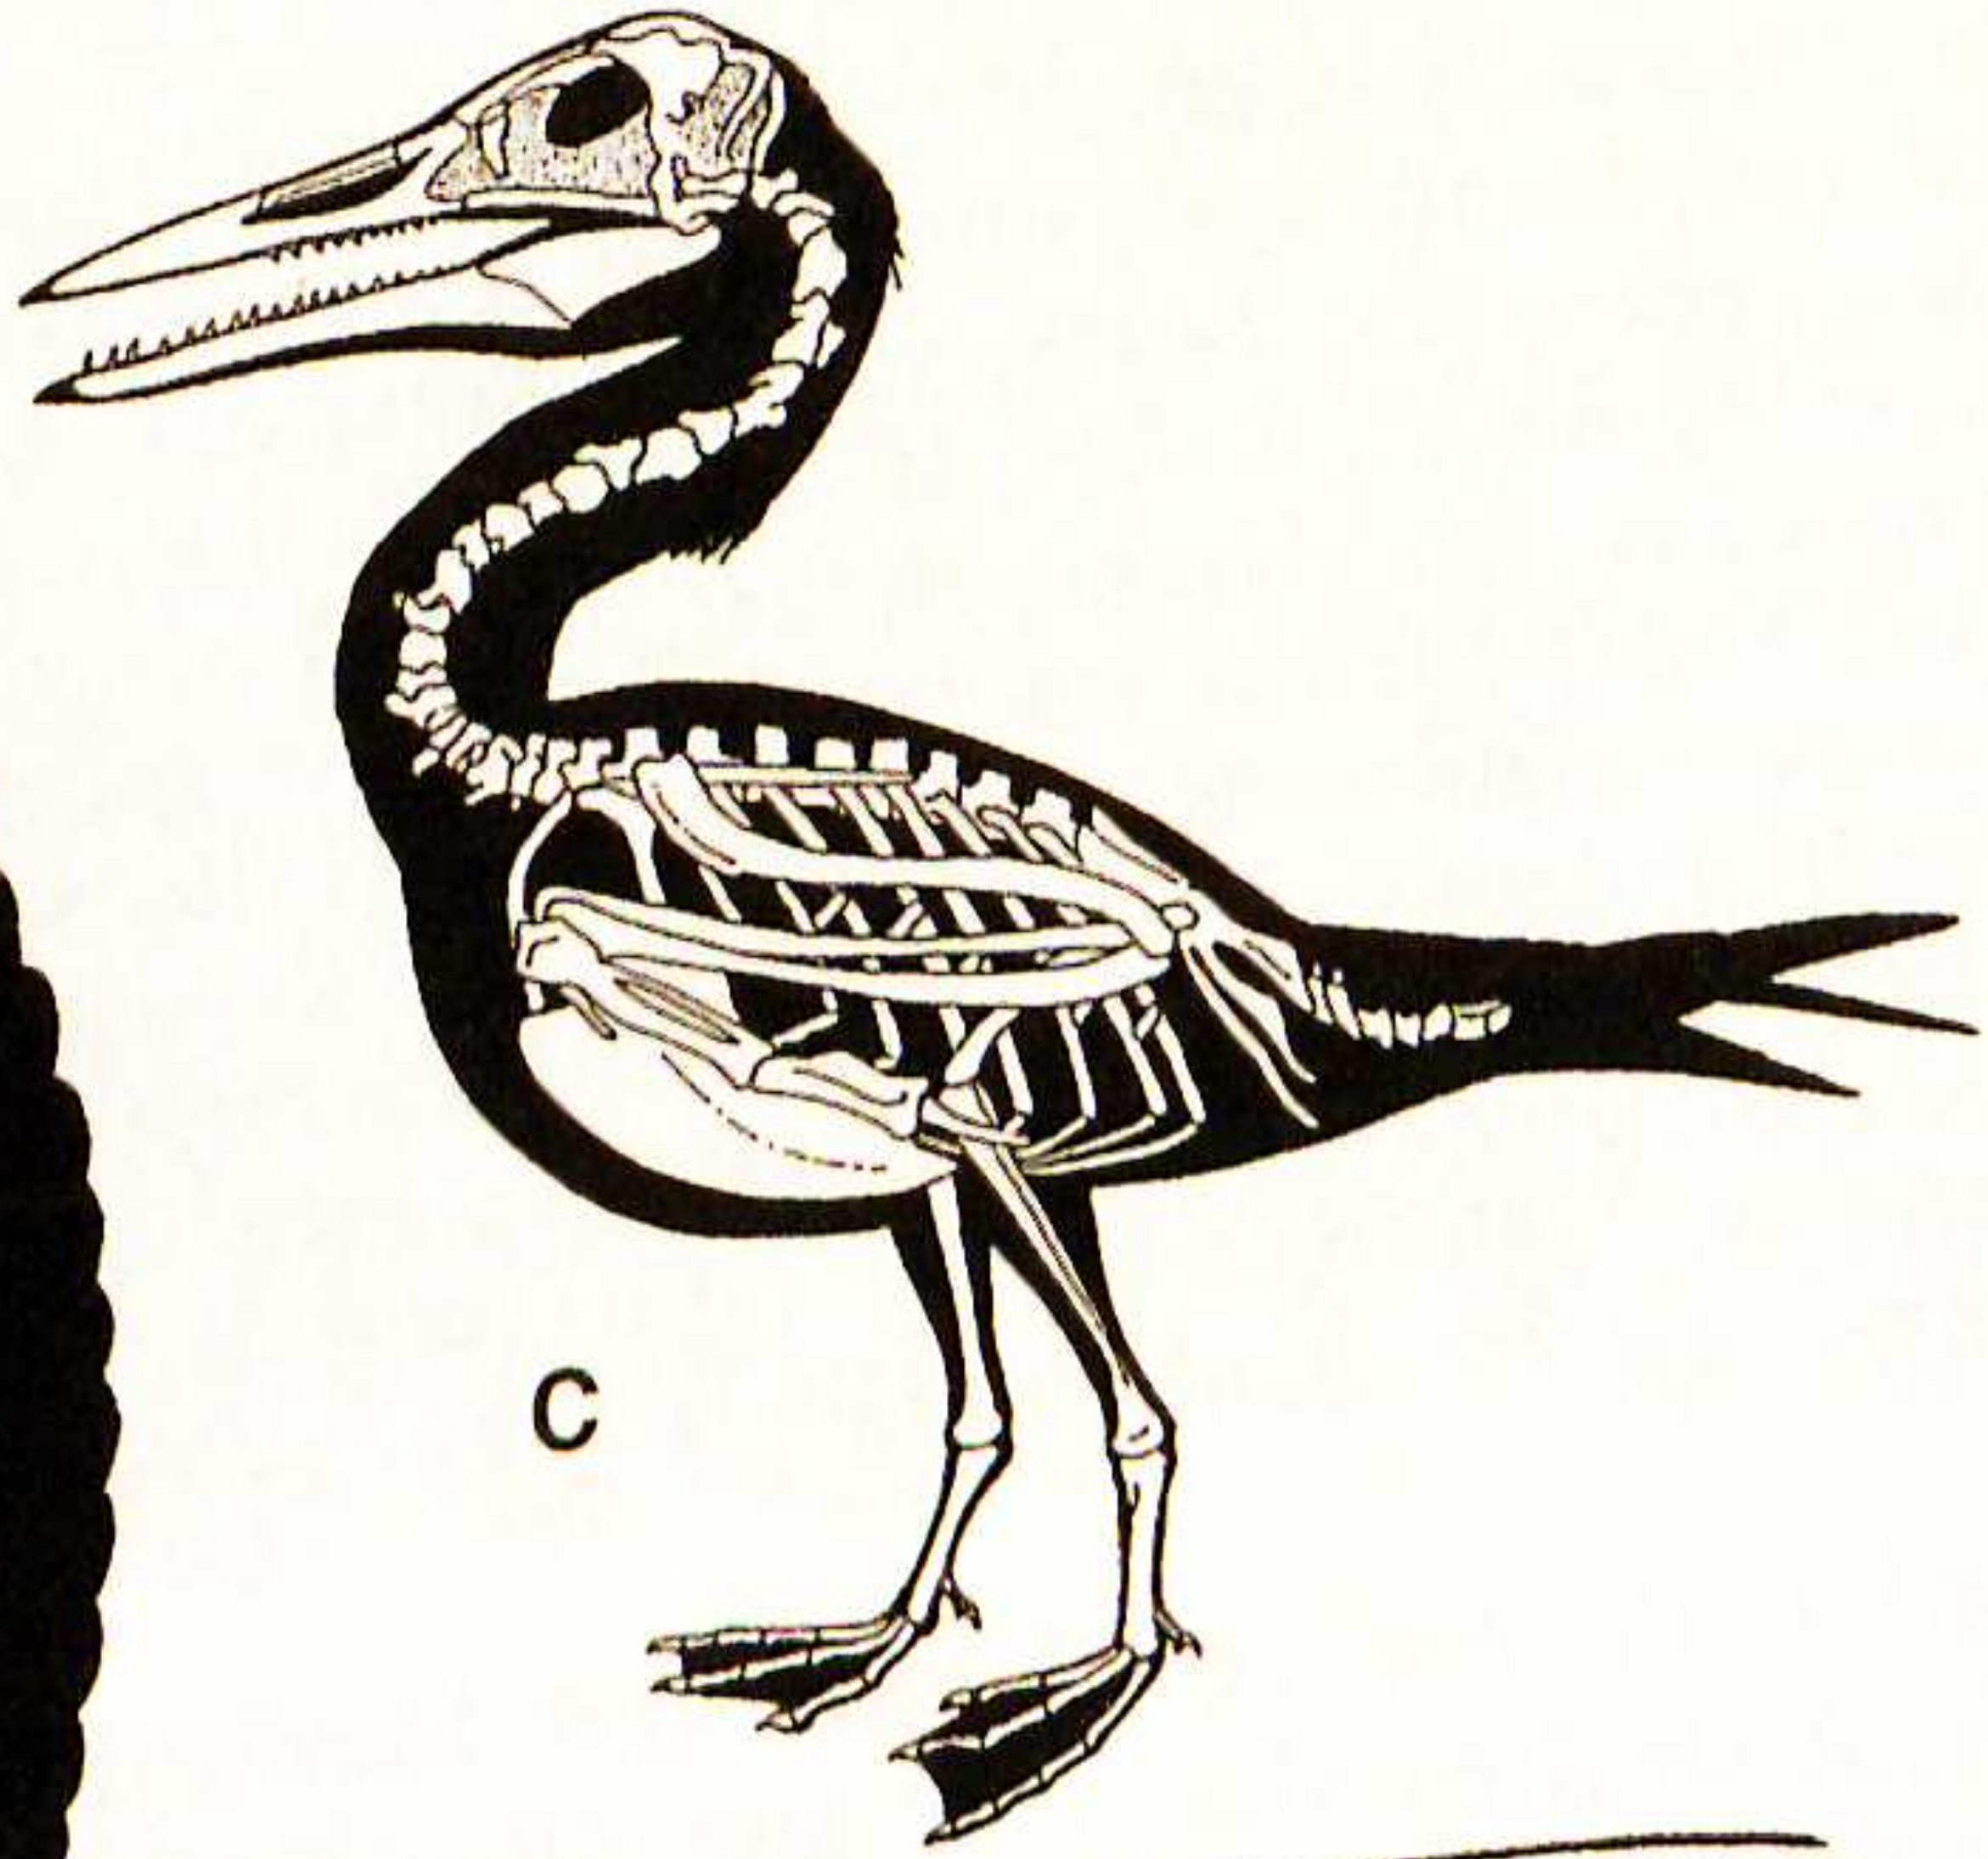
\includegraphics[width=0.2\textwidth]{../PCA/Skelettbilder_klein/Ichthyornis.jpg}}~
\subfloat[Ichthyosaurus]{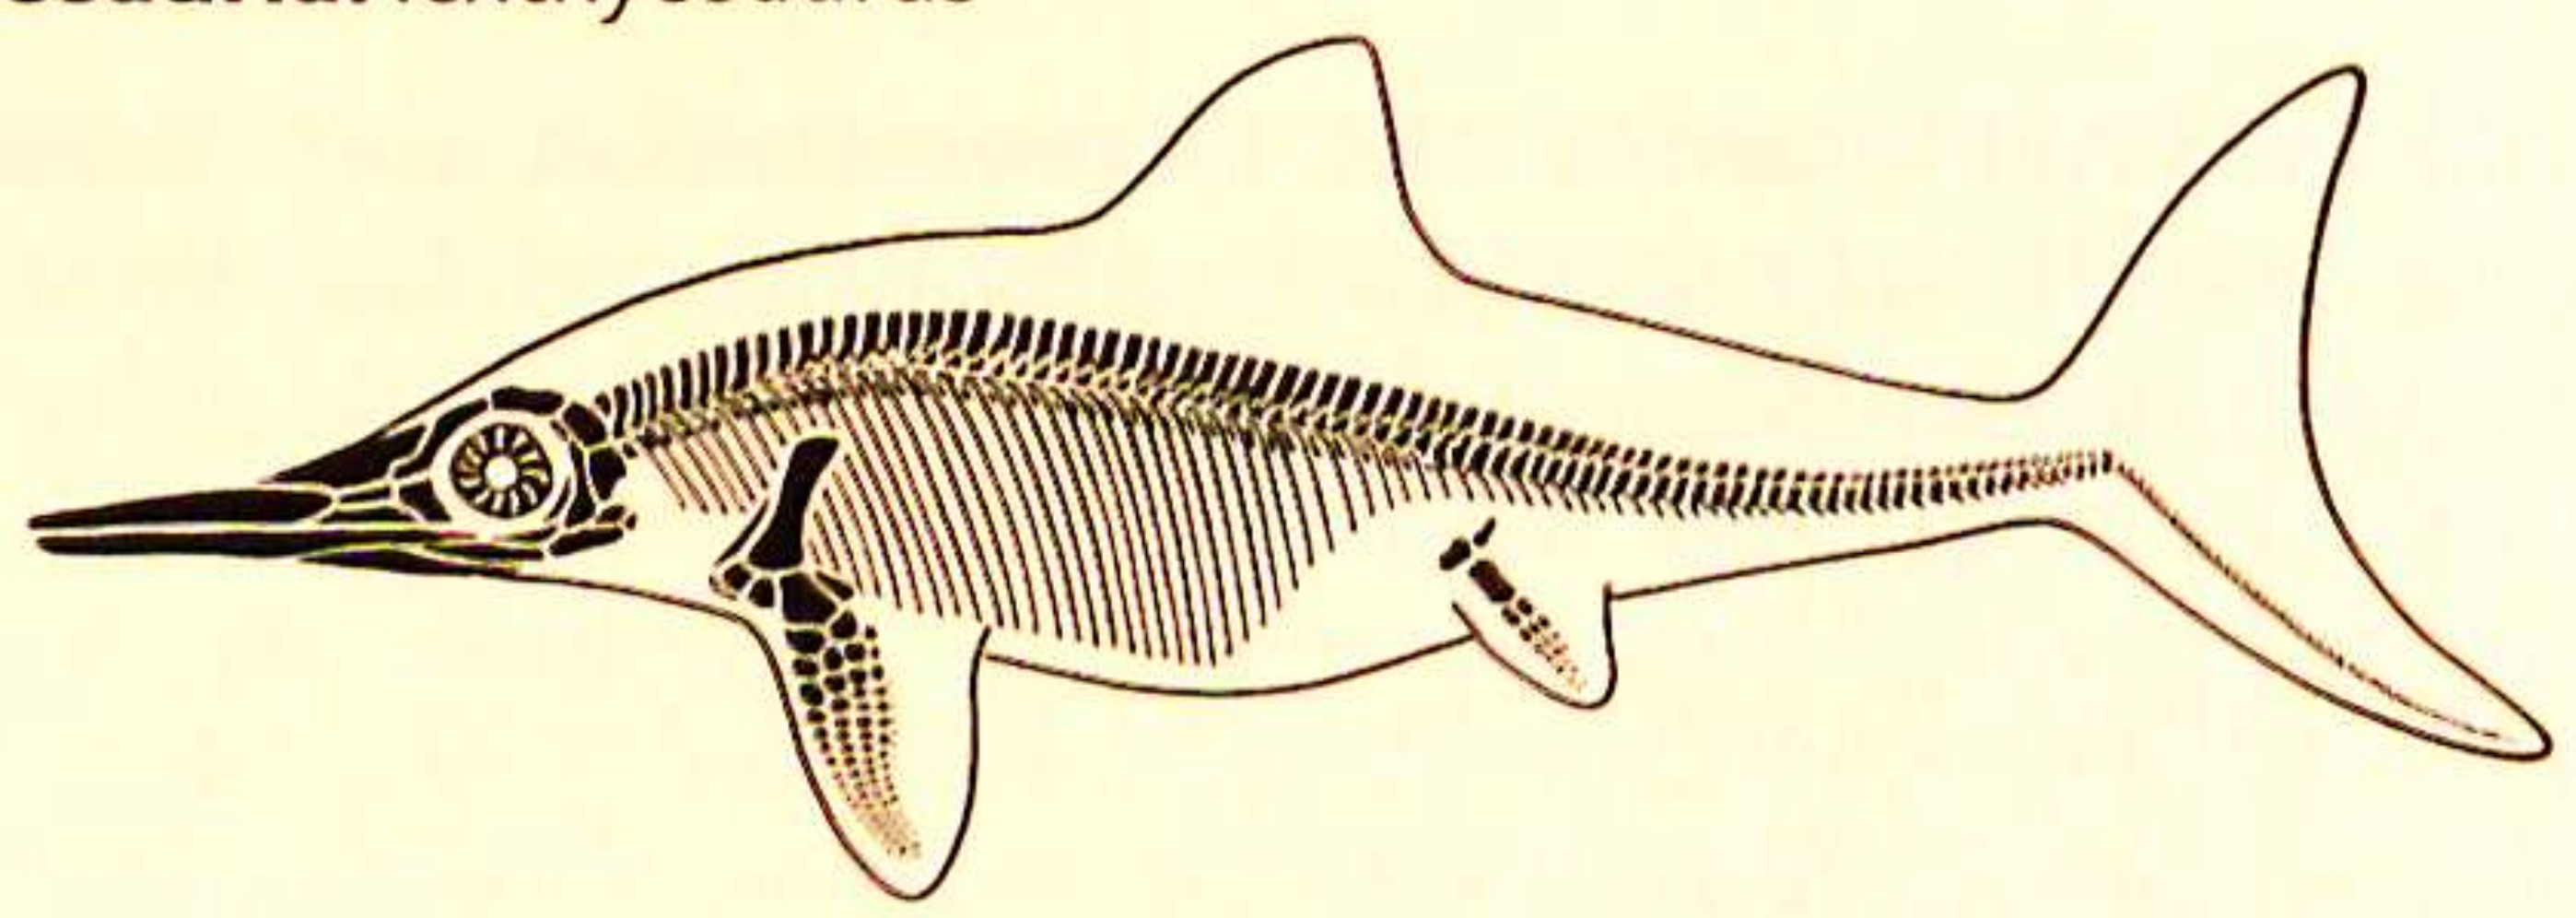
\includegraphics[width=0.2\textwidth]{../PCA/Skelettbilder_klein/Ichthyosaurus.jpg}}~
\subfloat[Ichthyostega]{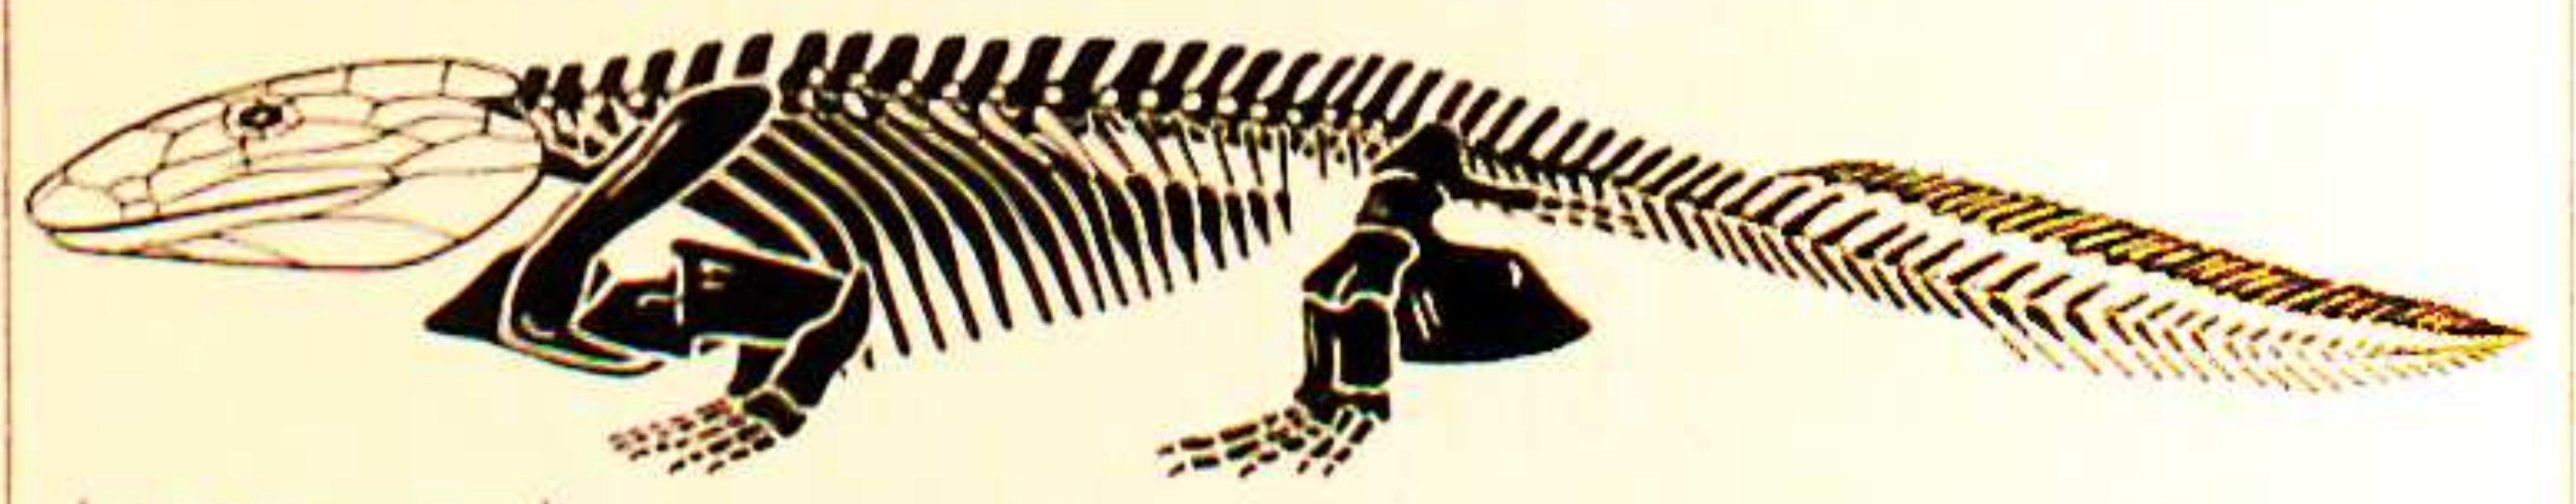
\includegraphics[width=0.2\textwidth]{../PCA/Skelettbilder_klein/Ichthyostega.jpg}}~
\subfloat[Känguru]{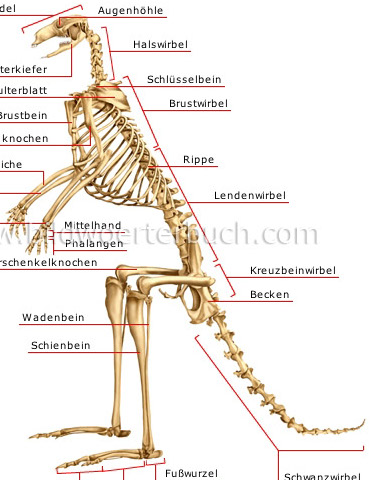
\includegraphics[width=0.2\textwidth]{../PCA/Skelettbilder_klein/Kaenguru.jpg}}~
\subfloat[Kaffernbüffel]{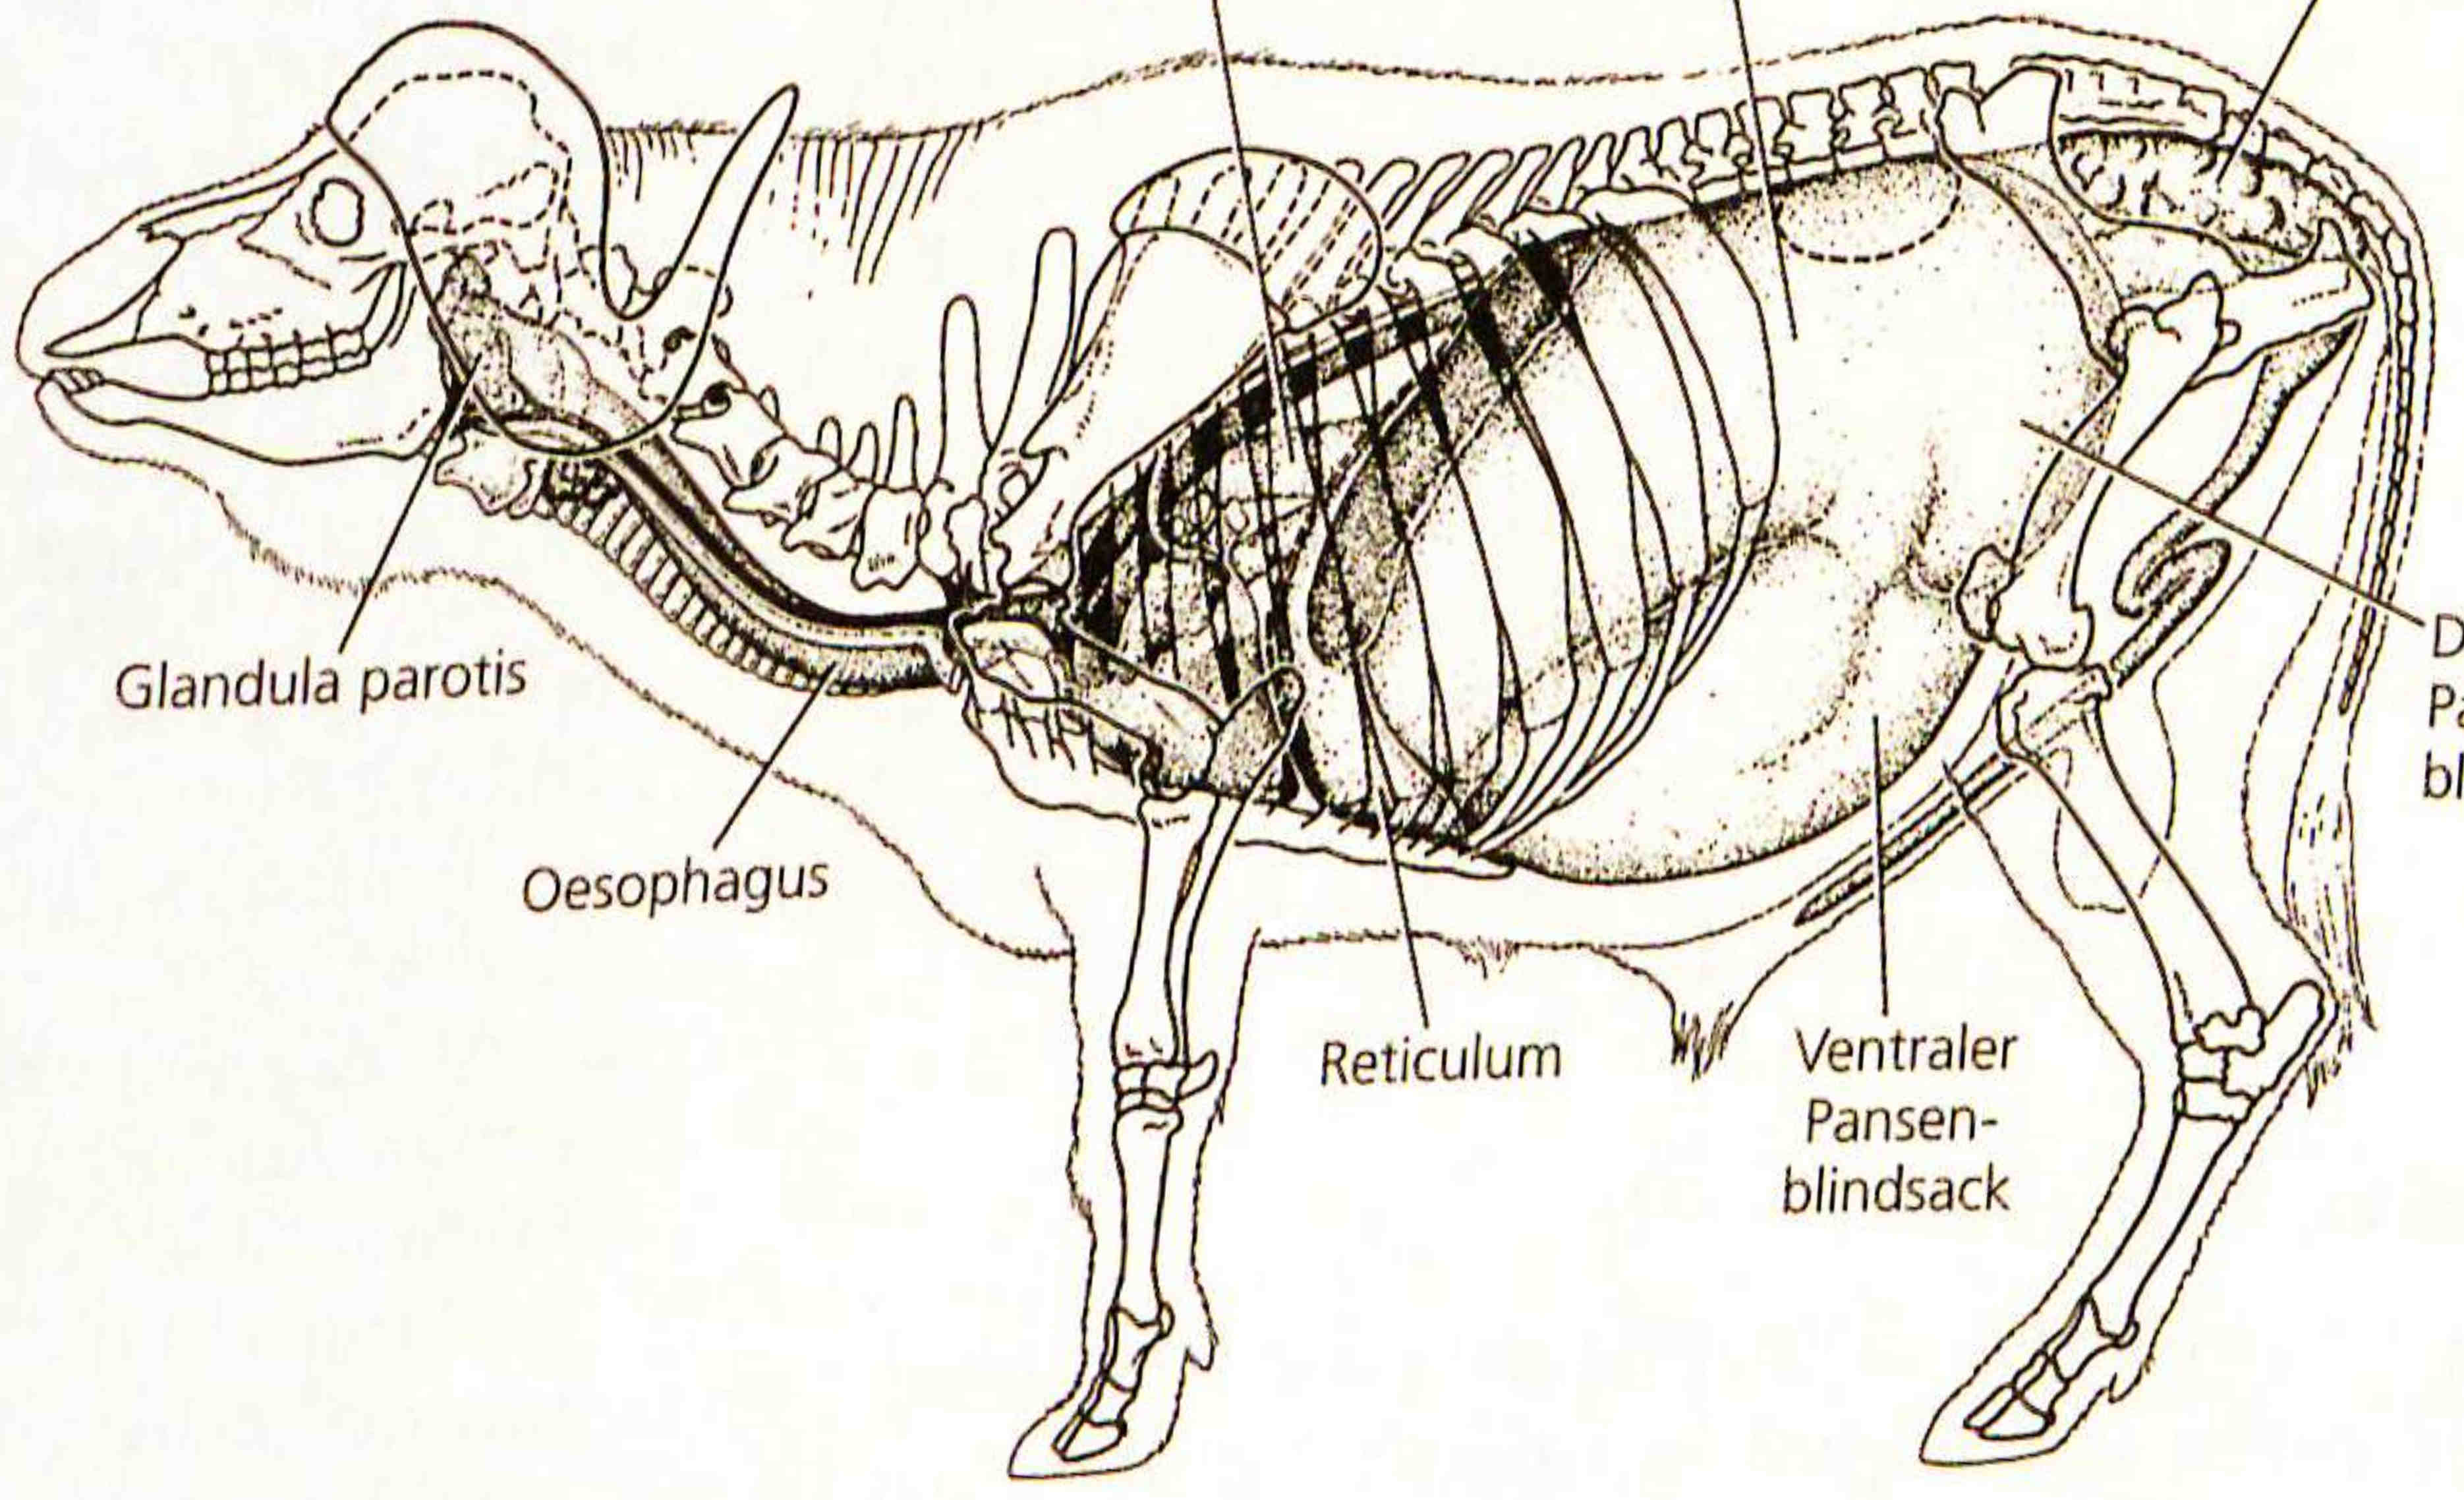
\includegraphics[width=0.2\textwidth]{../PCA/Skelettbilder_klein/Kaffernbueffel.jpg}}
\\
\subfloat[Kaninchen]{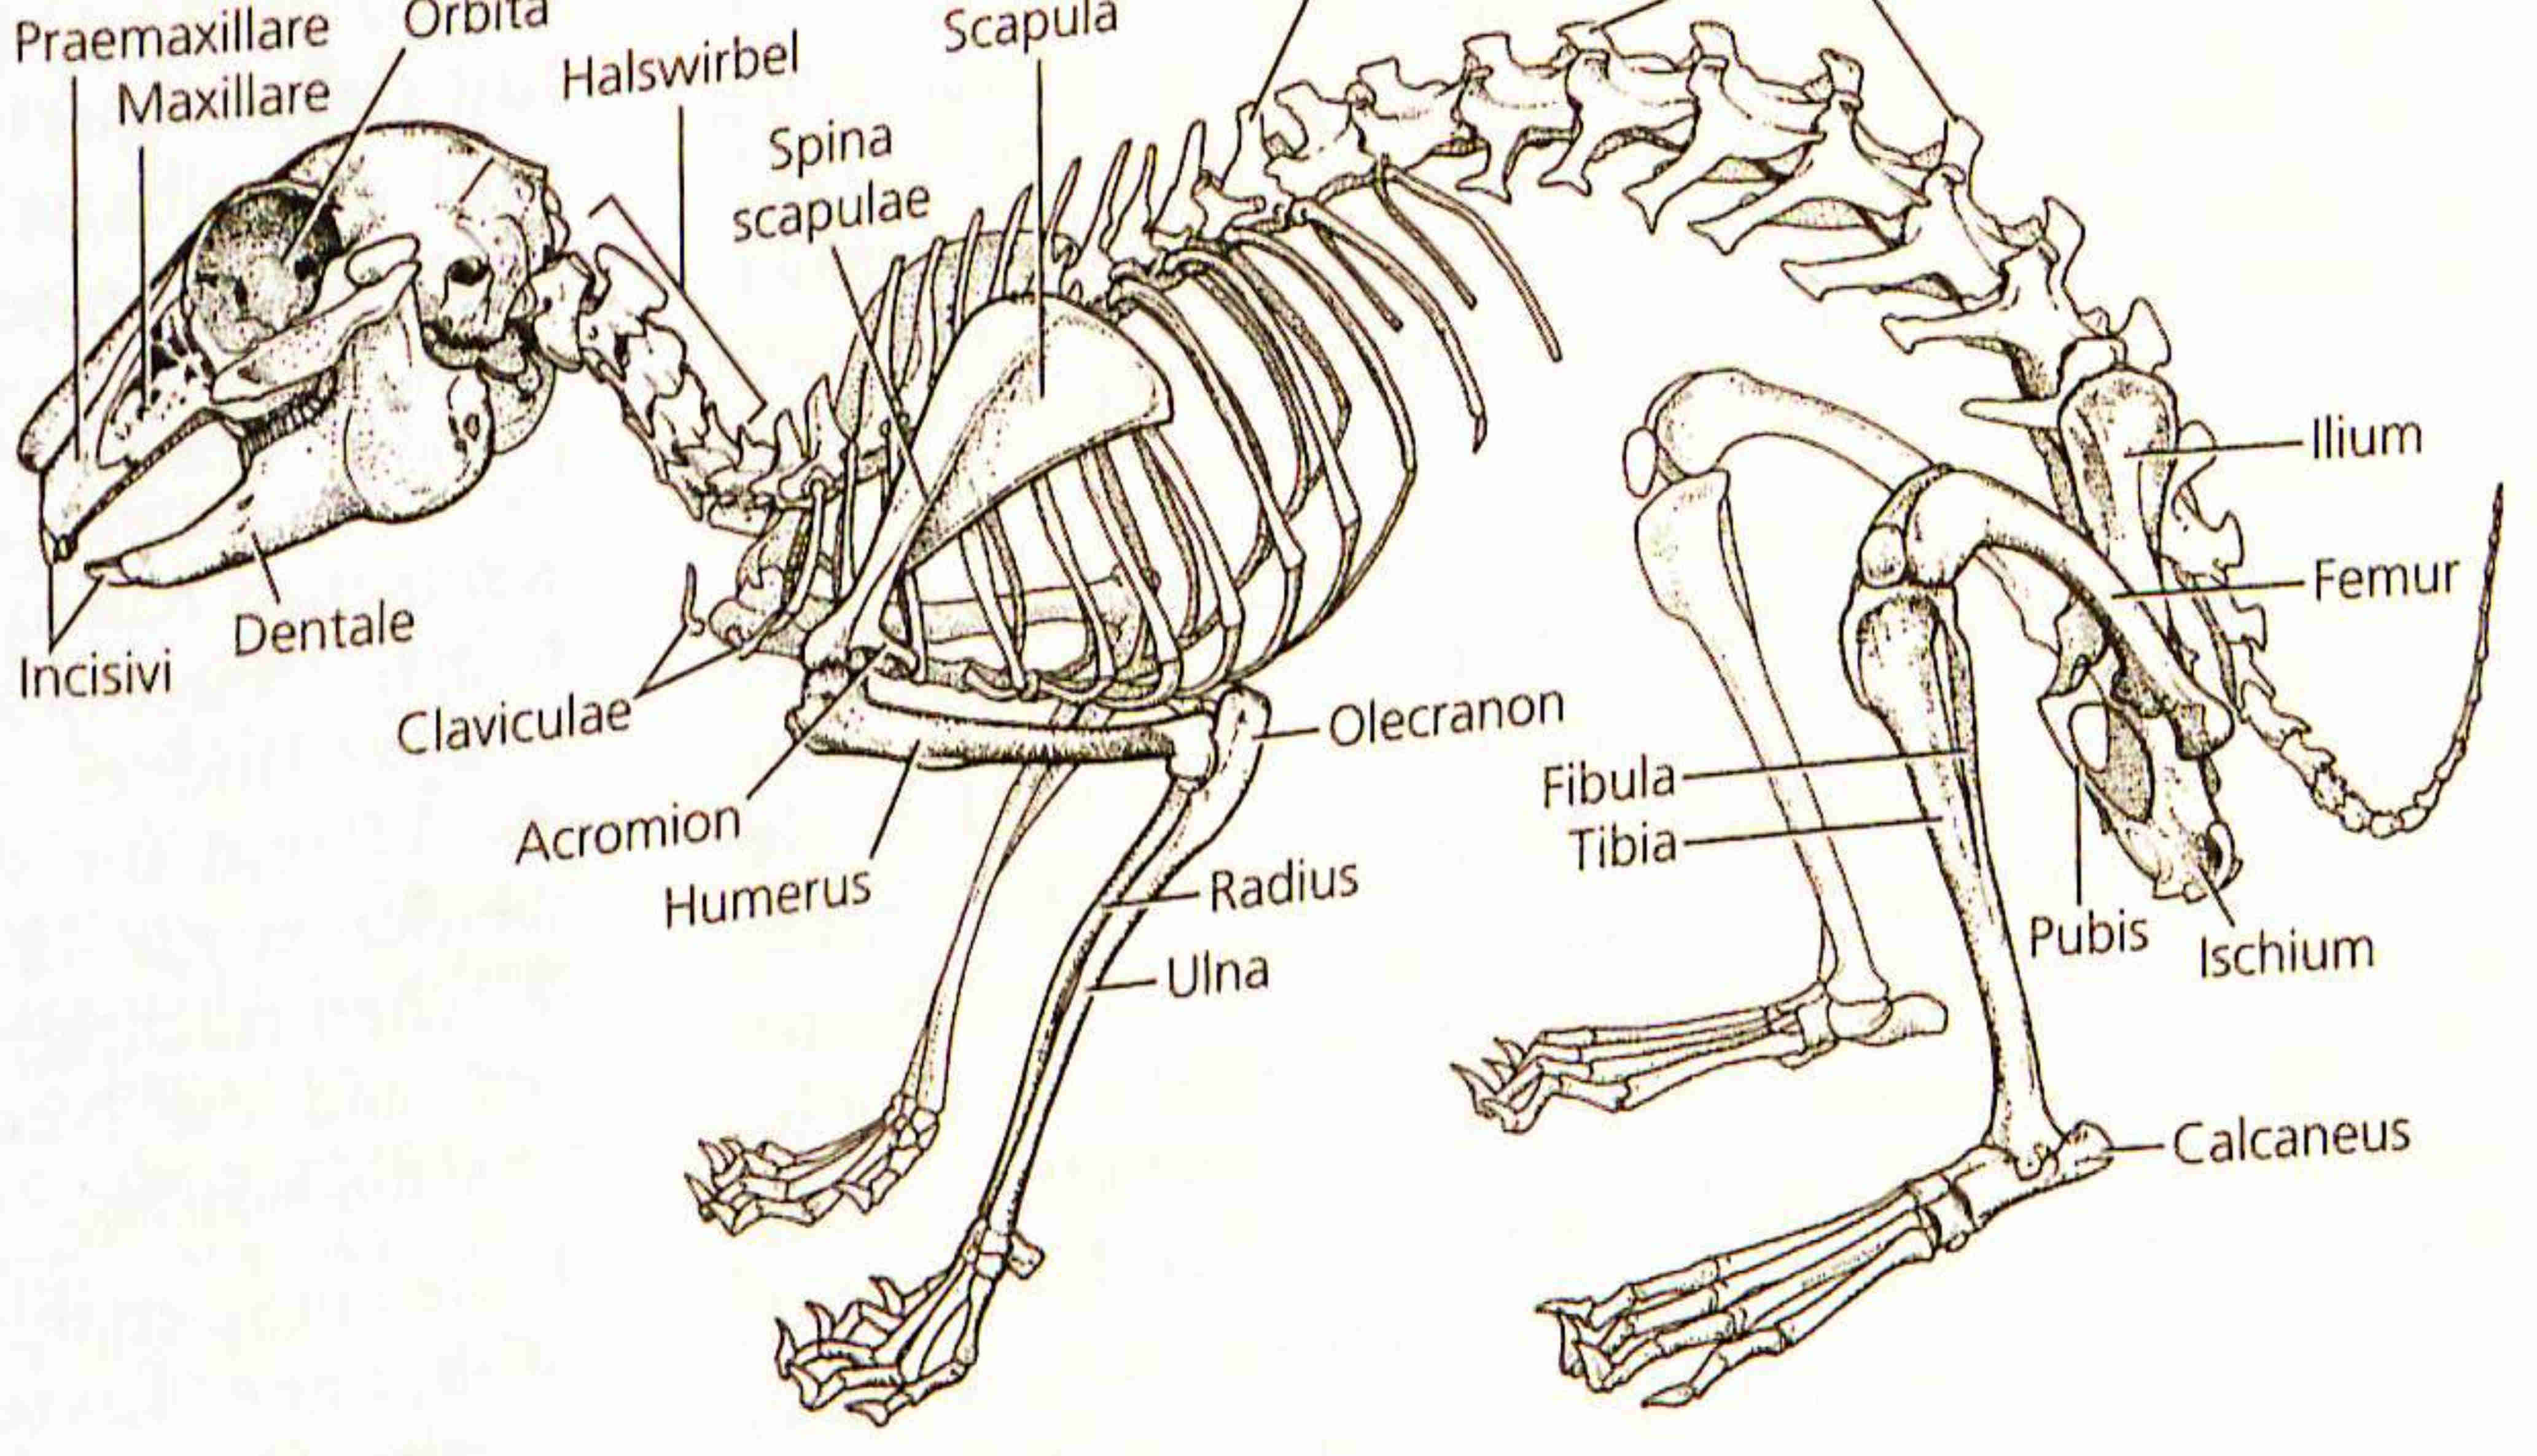
\includegraphics[width=0.2\textwidth]{../PCA/Skelettbilder_klein/Kaninchen.jpg}}~
\subfloat[Klippschliefer]{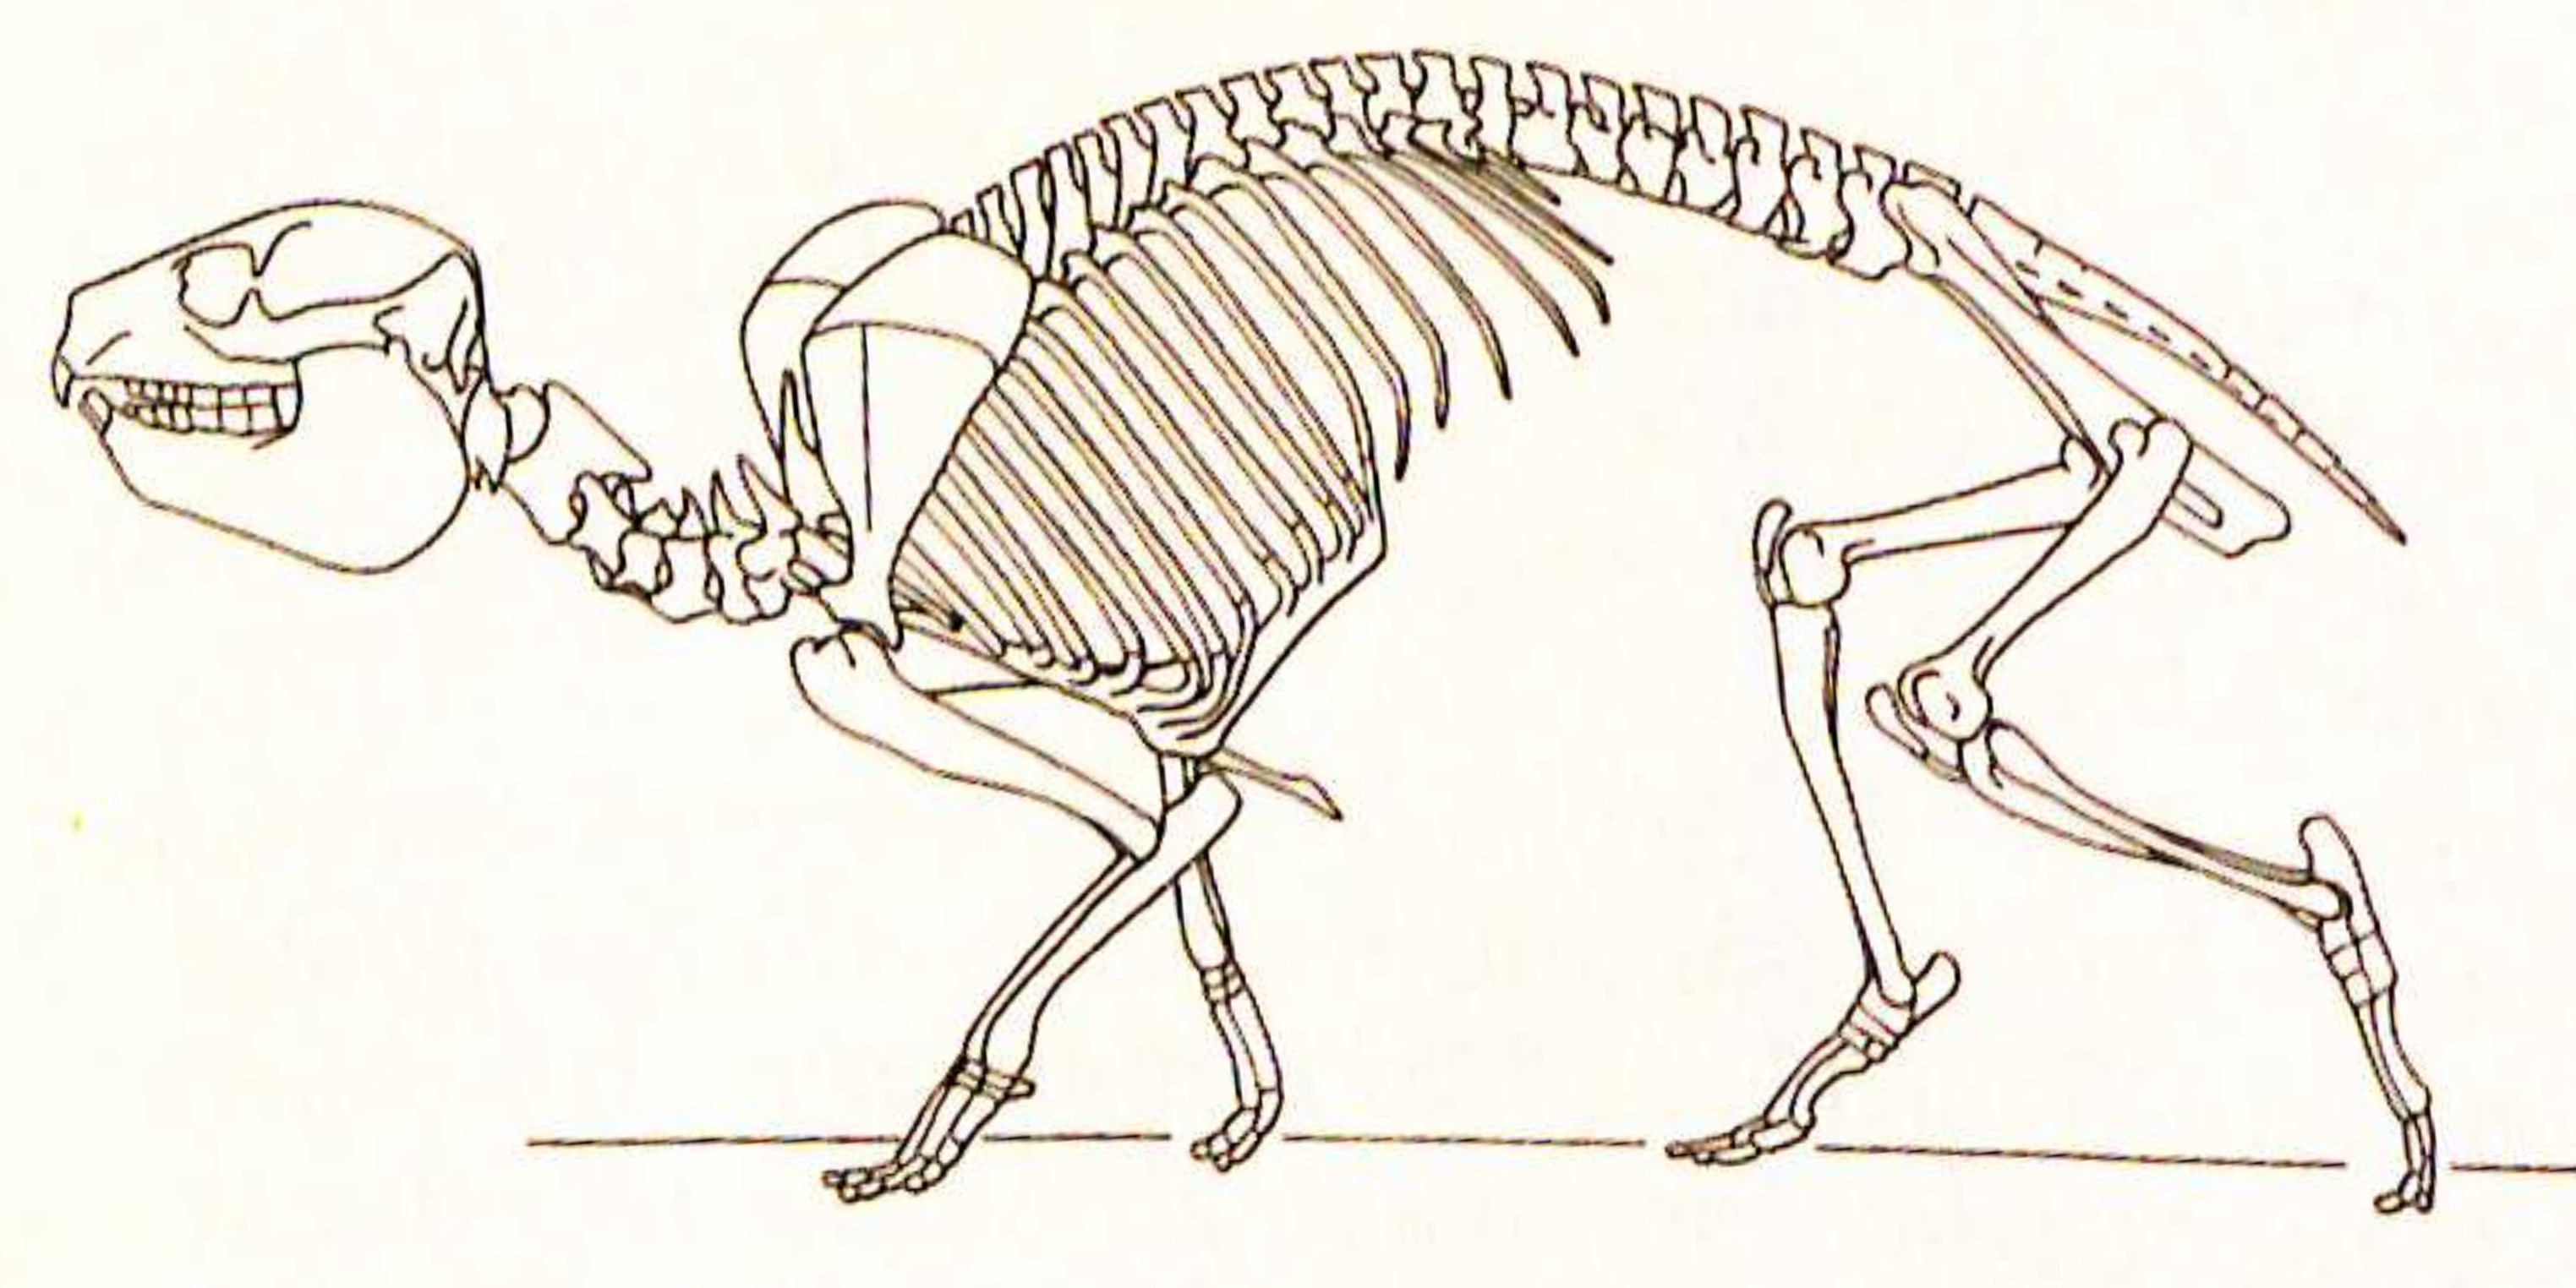
\includegraphics[width=0.2\textwidth]{../PCA/Skelettbilder_klein/Klippschliefer.jpg}}~
\subfloat[Koboldmaki]{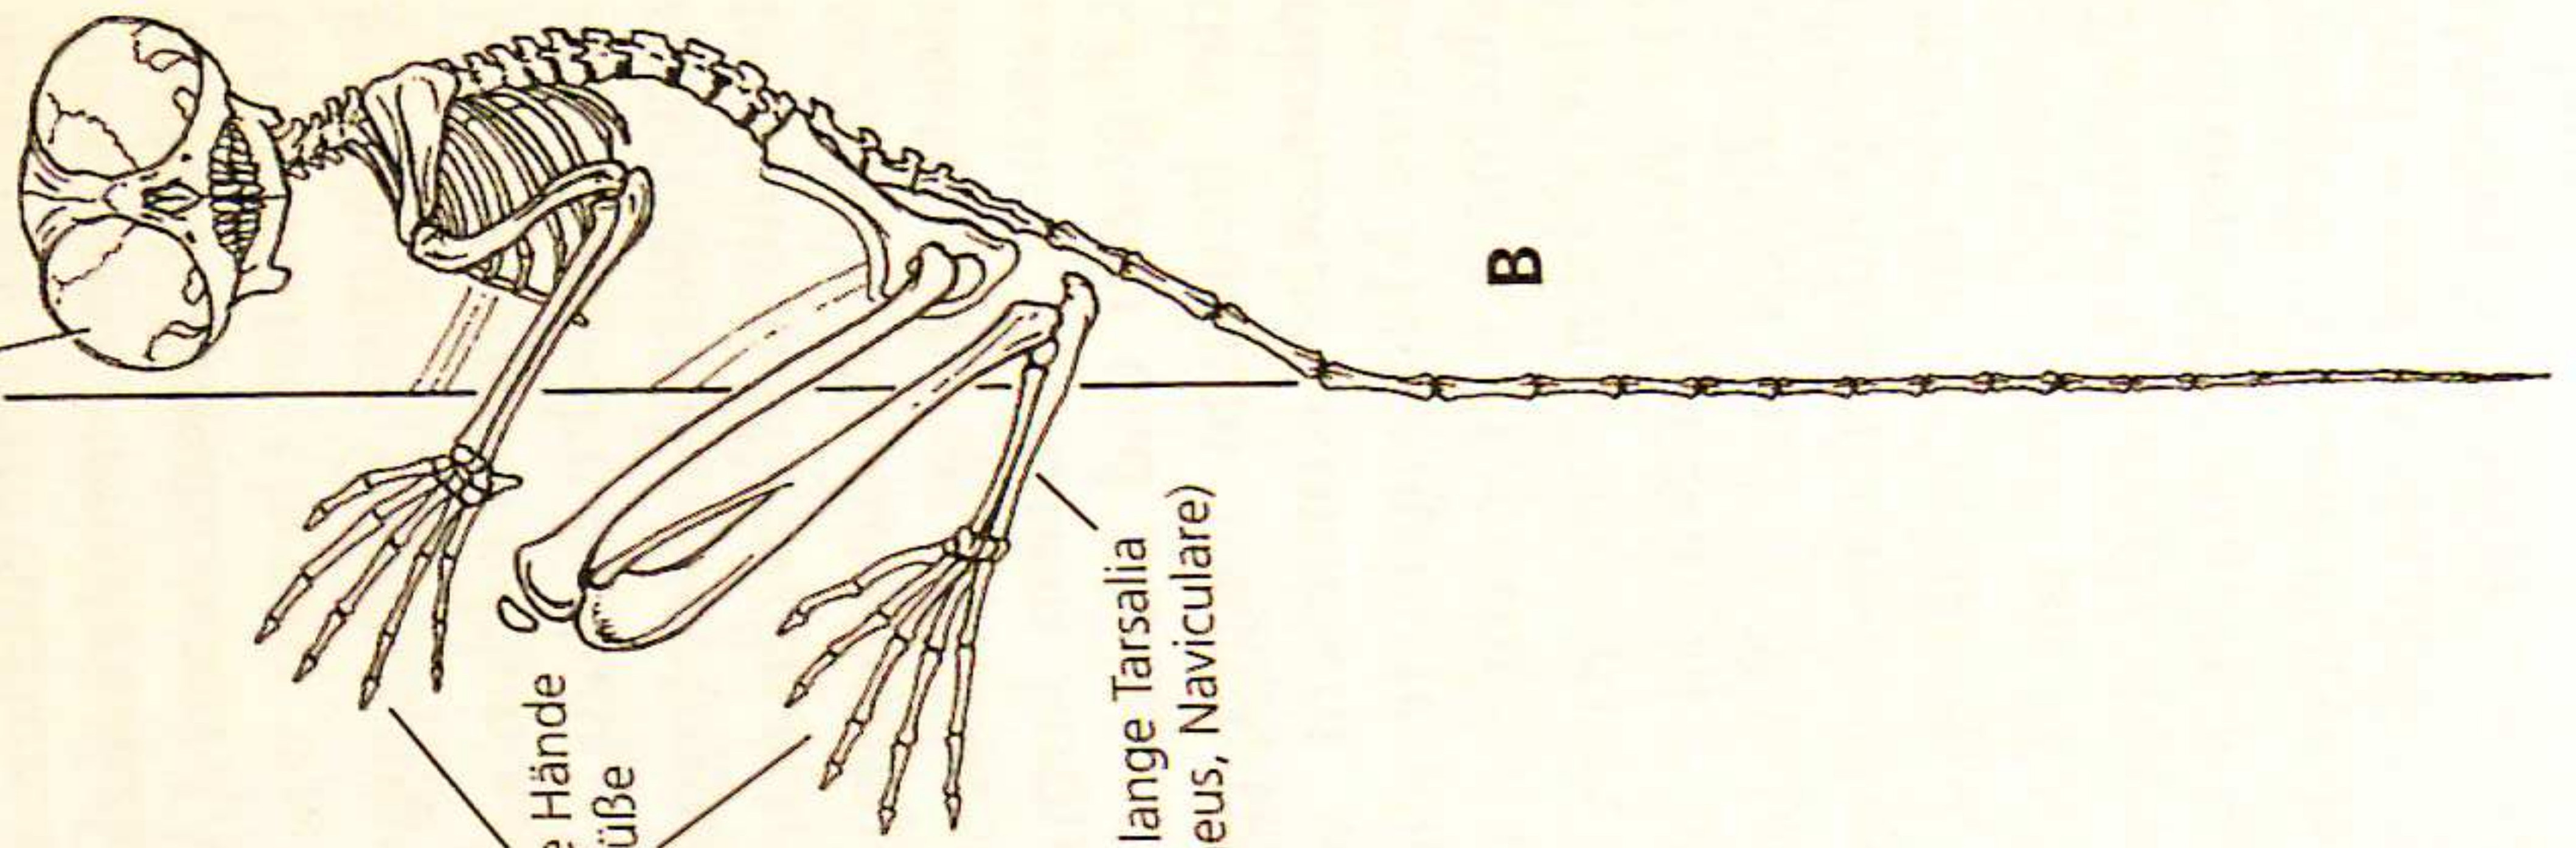
\includegraphics[width=0.2\textwidth]{../PCA/Skelettbilder_klein/Koboldmaki.jpg}}~
\subfloat[Krokodil]{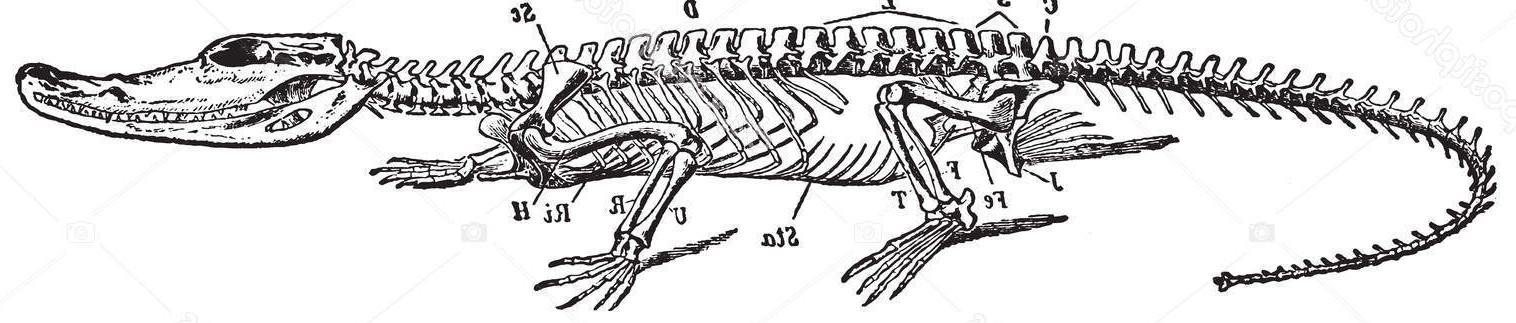
\includegraphics[width=0.2\textwidth]{../PCA/Skelettbilder_klein/Krokodil.jpg}}~
\subfloat[Landschildkröte]{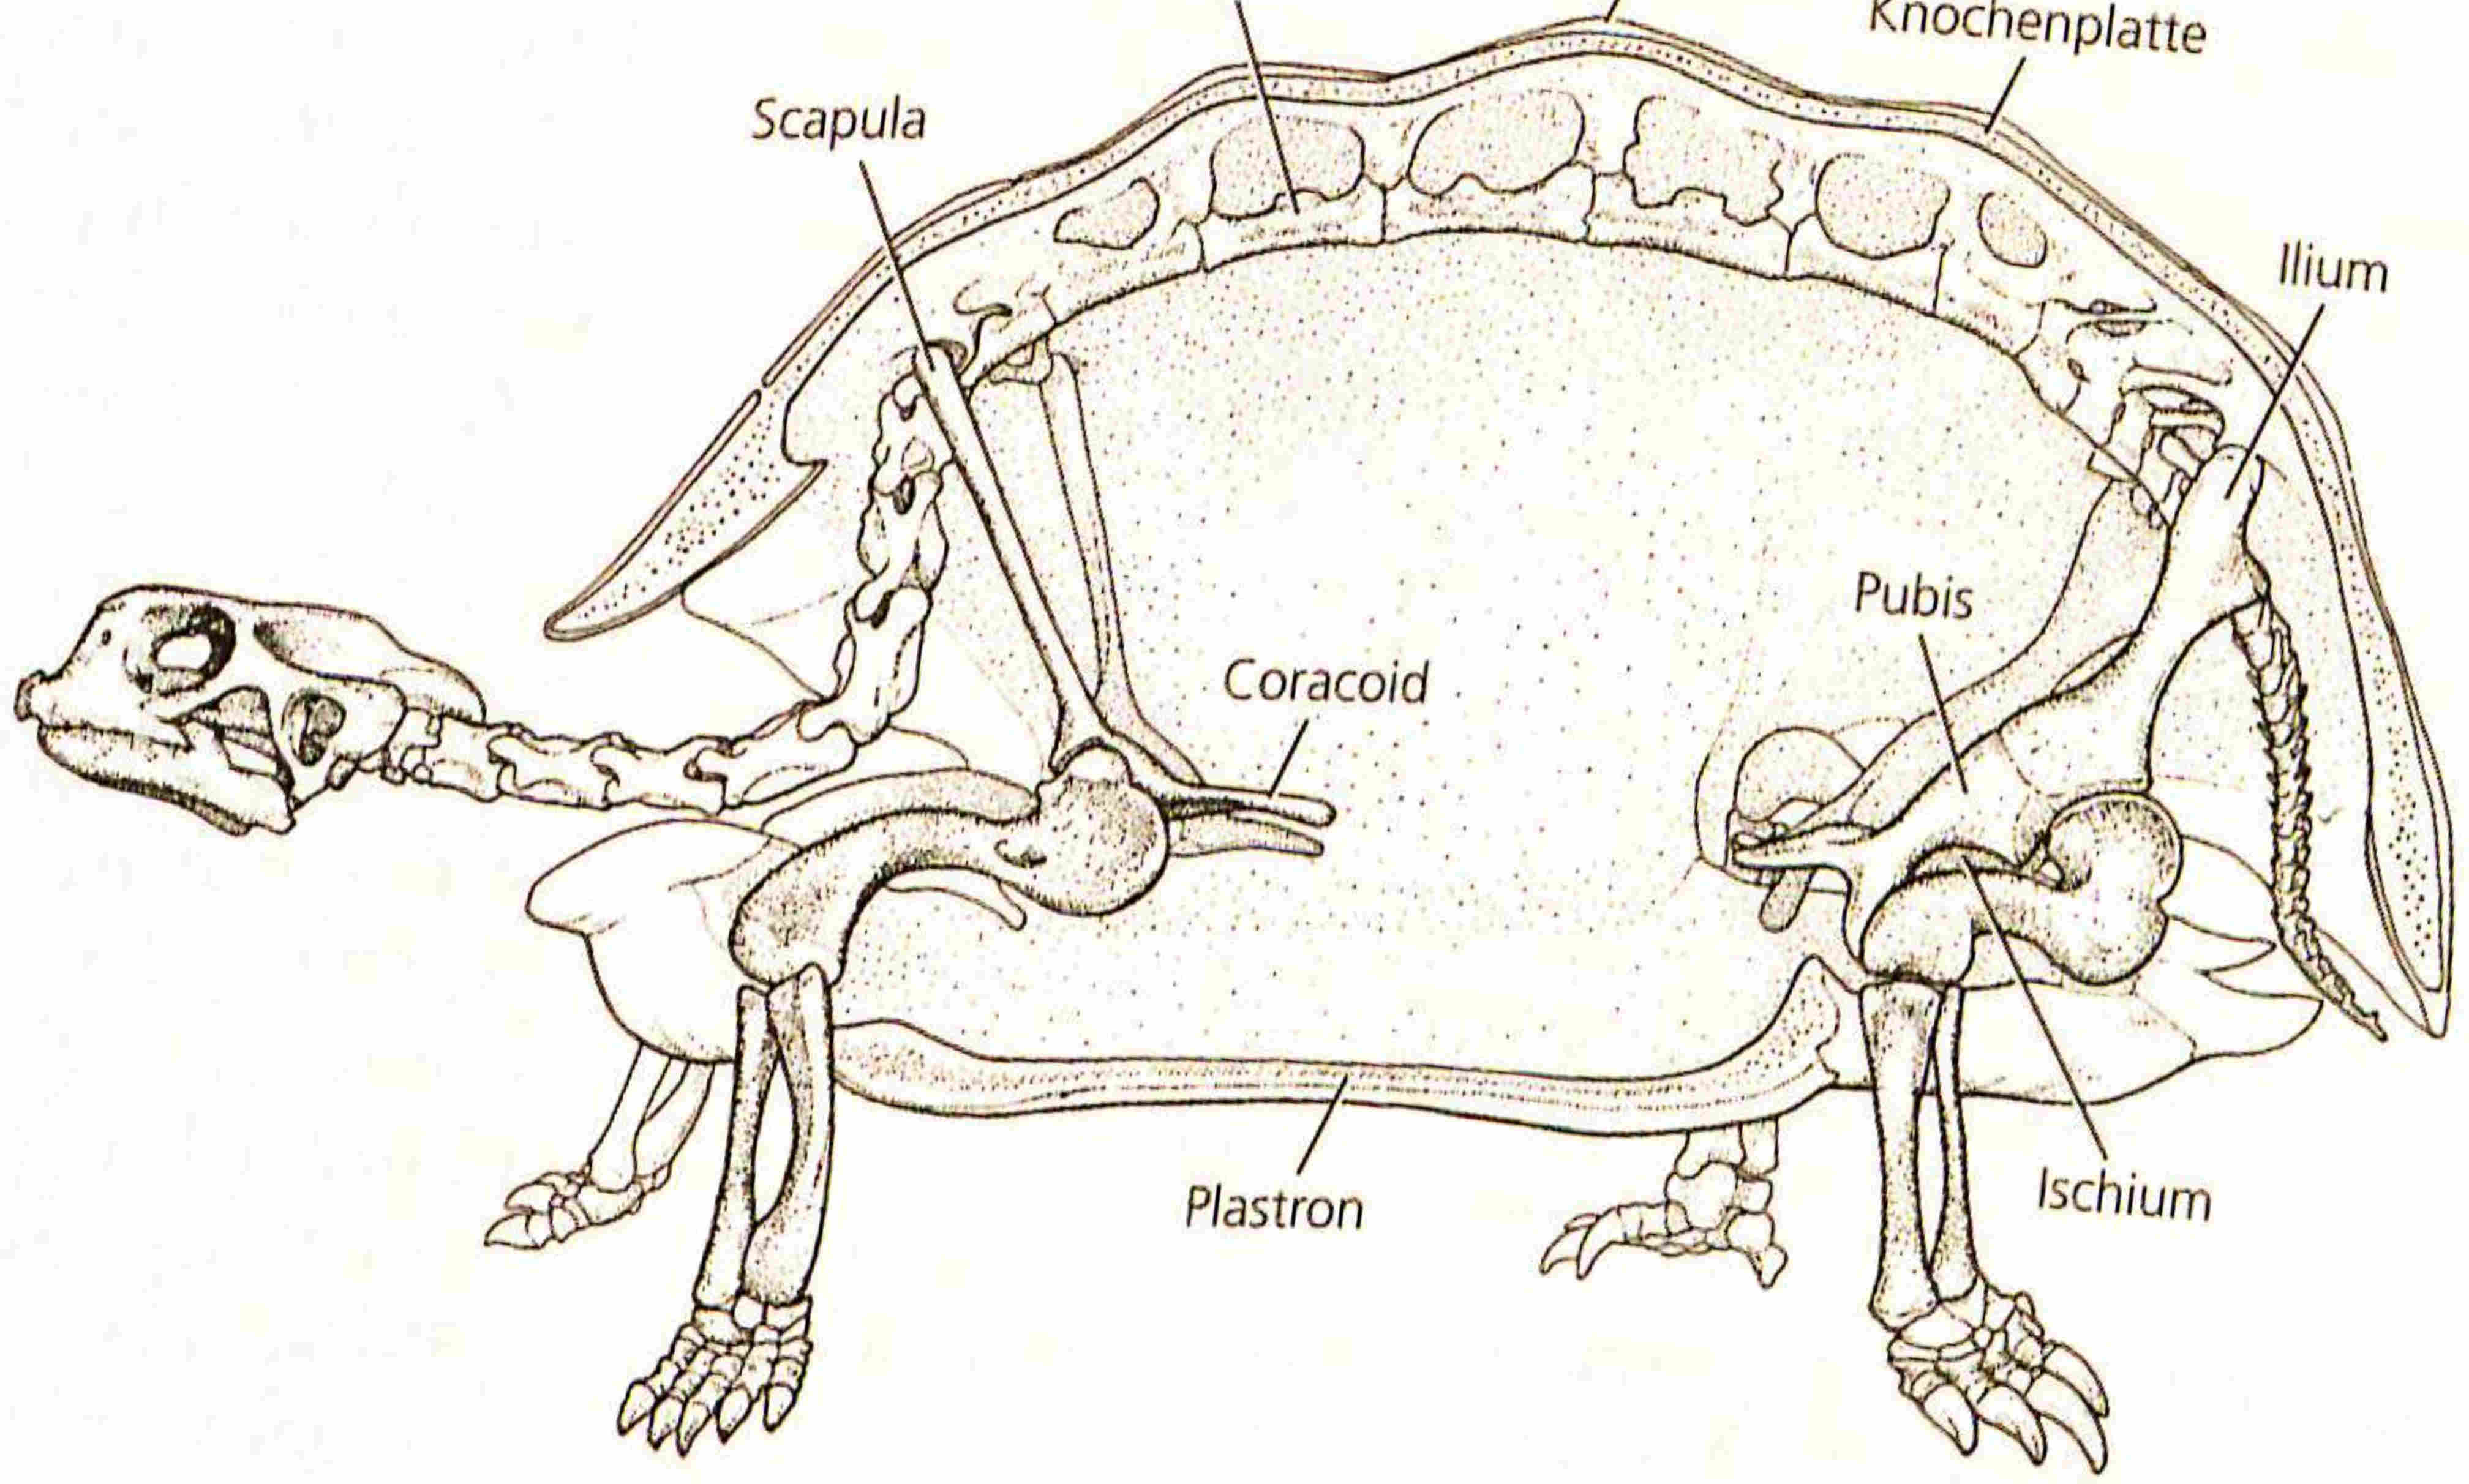
\includegraphics[width=0.2\textwidth]{../PCA/Skelettbilder_klein/Landschildkroete.jpg}}
\phantomcaption

\end{figure}
\begin{figure}
\ContinuedFloat

\subfloat[Ohrenrobbe]{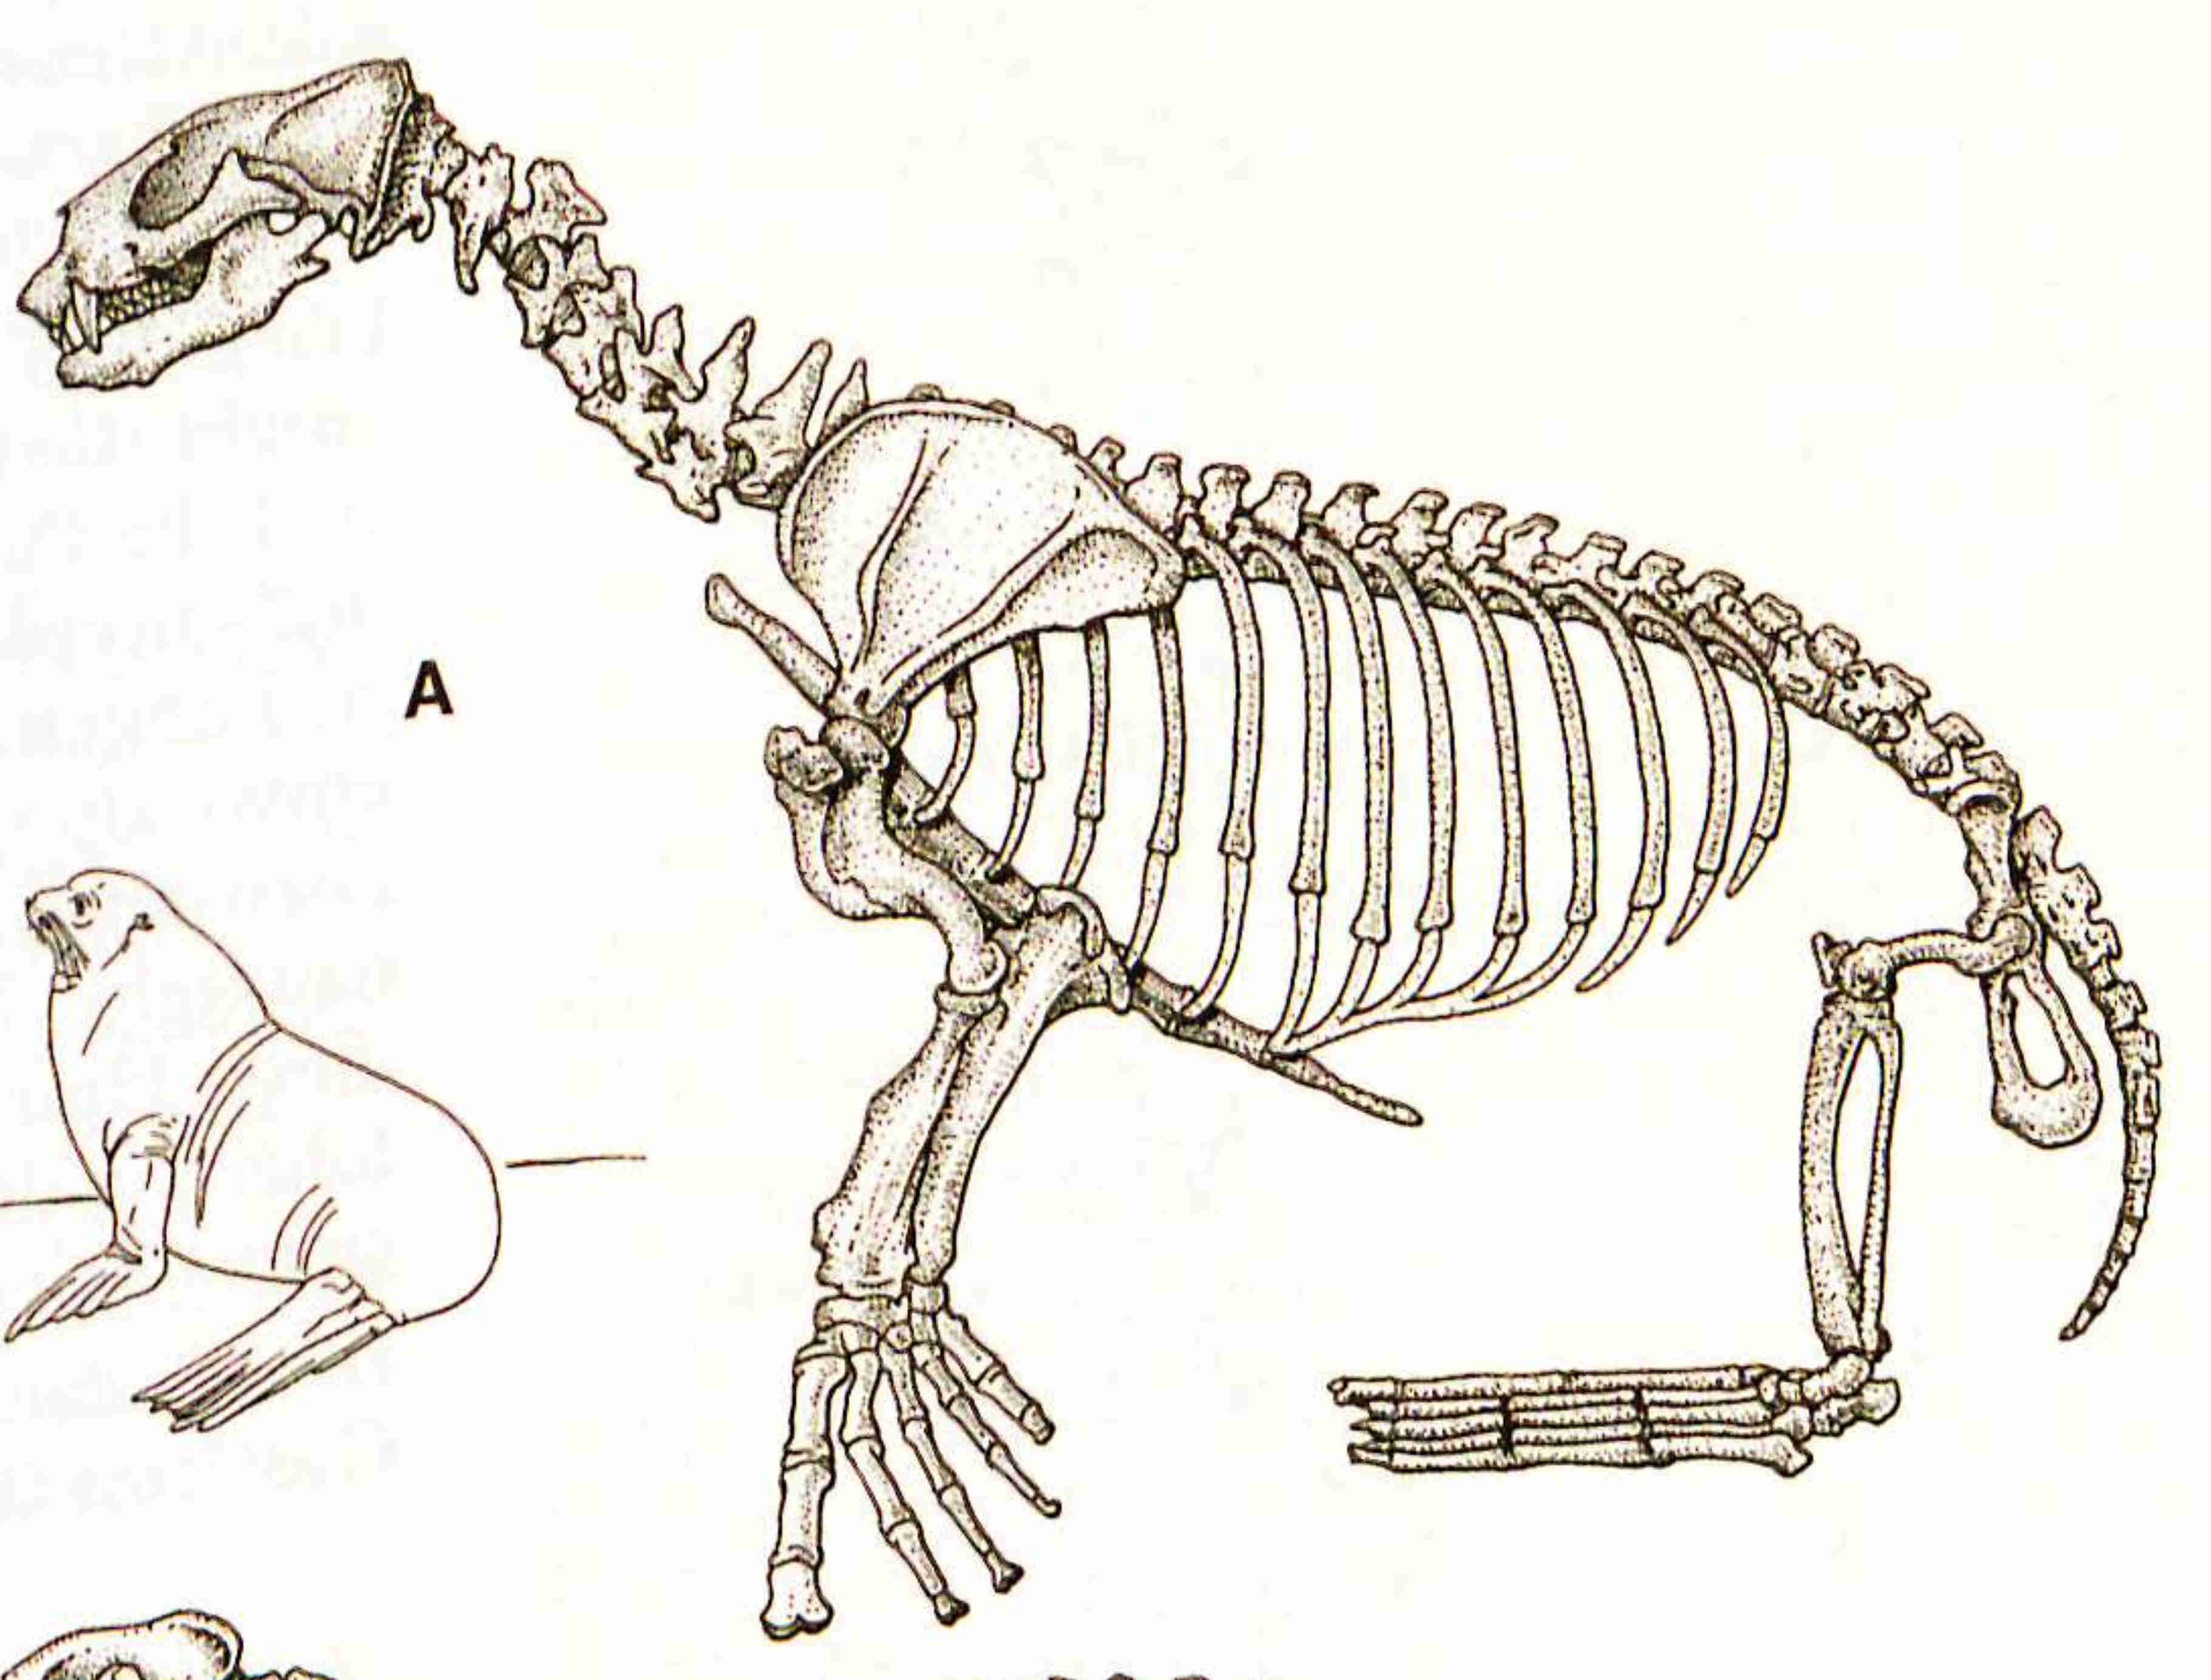
\includegraphics[width=0.2\textwidth]{../PCA/Skelettbilder_klein/Ohrenrobbe.jpg}}~
\subfloat[Panzerspitzmaus]{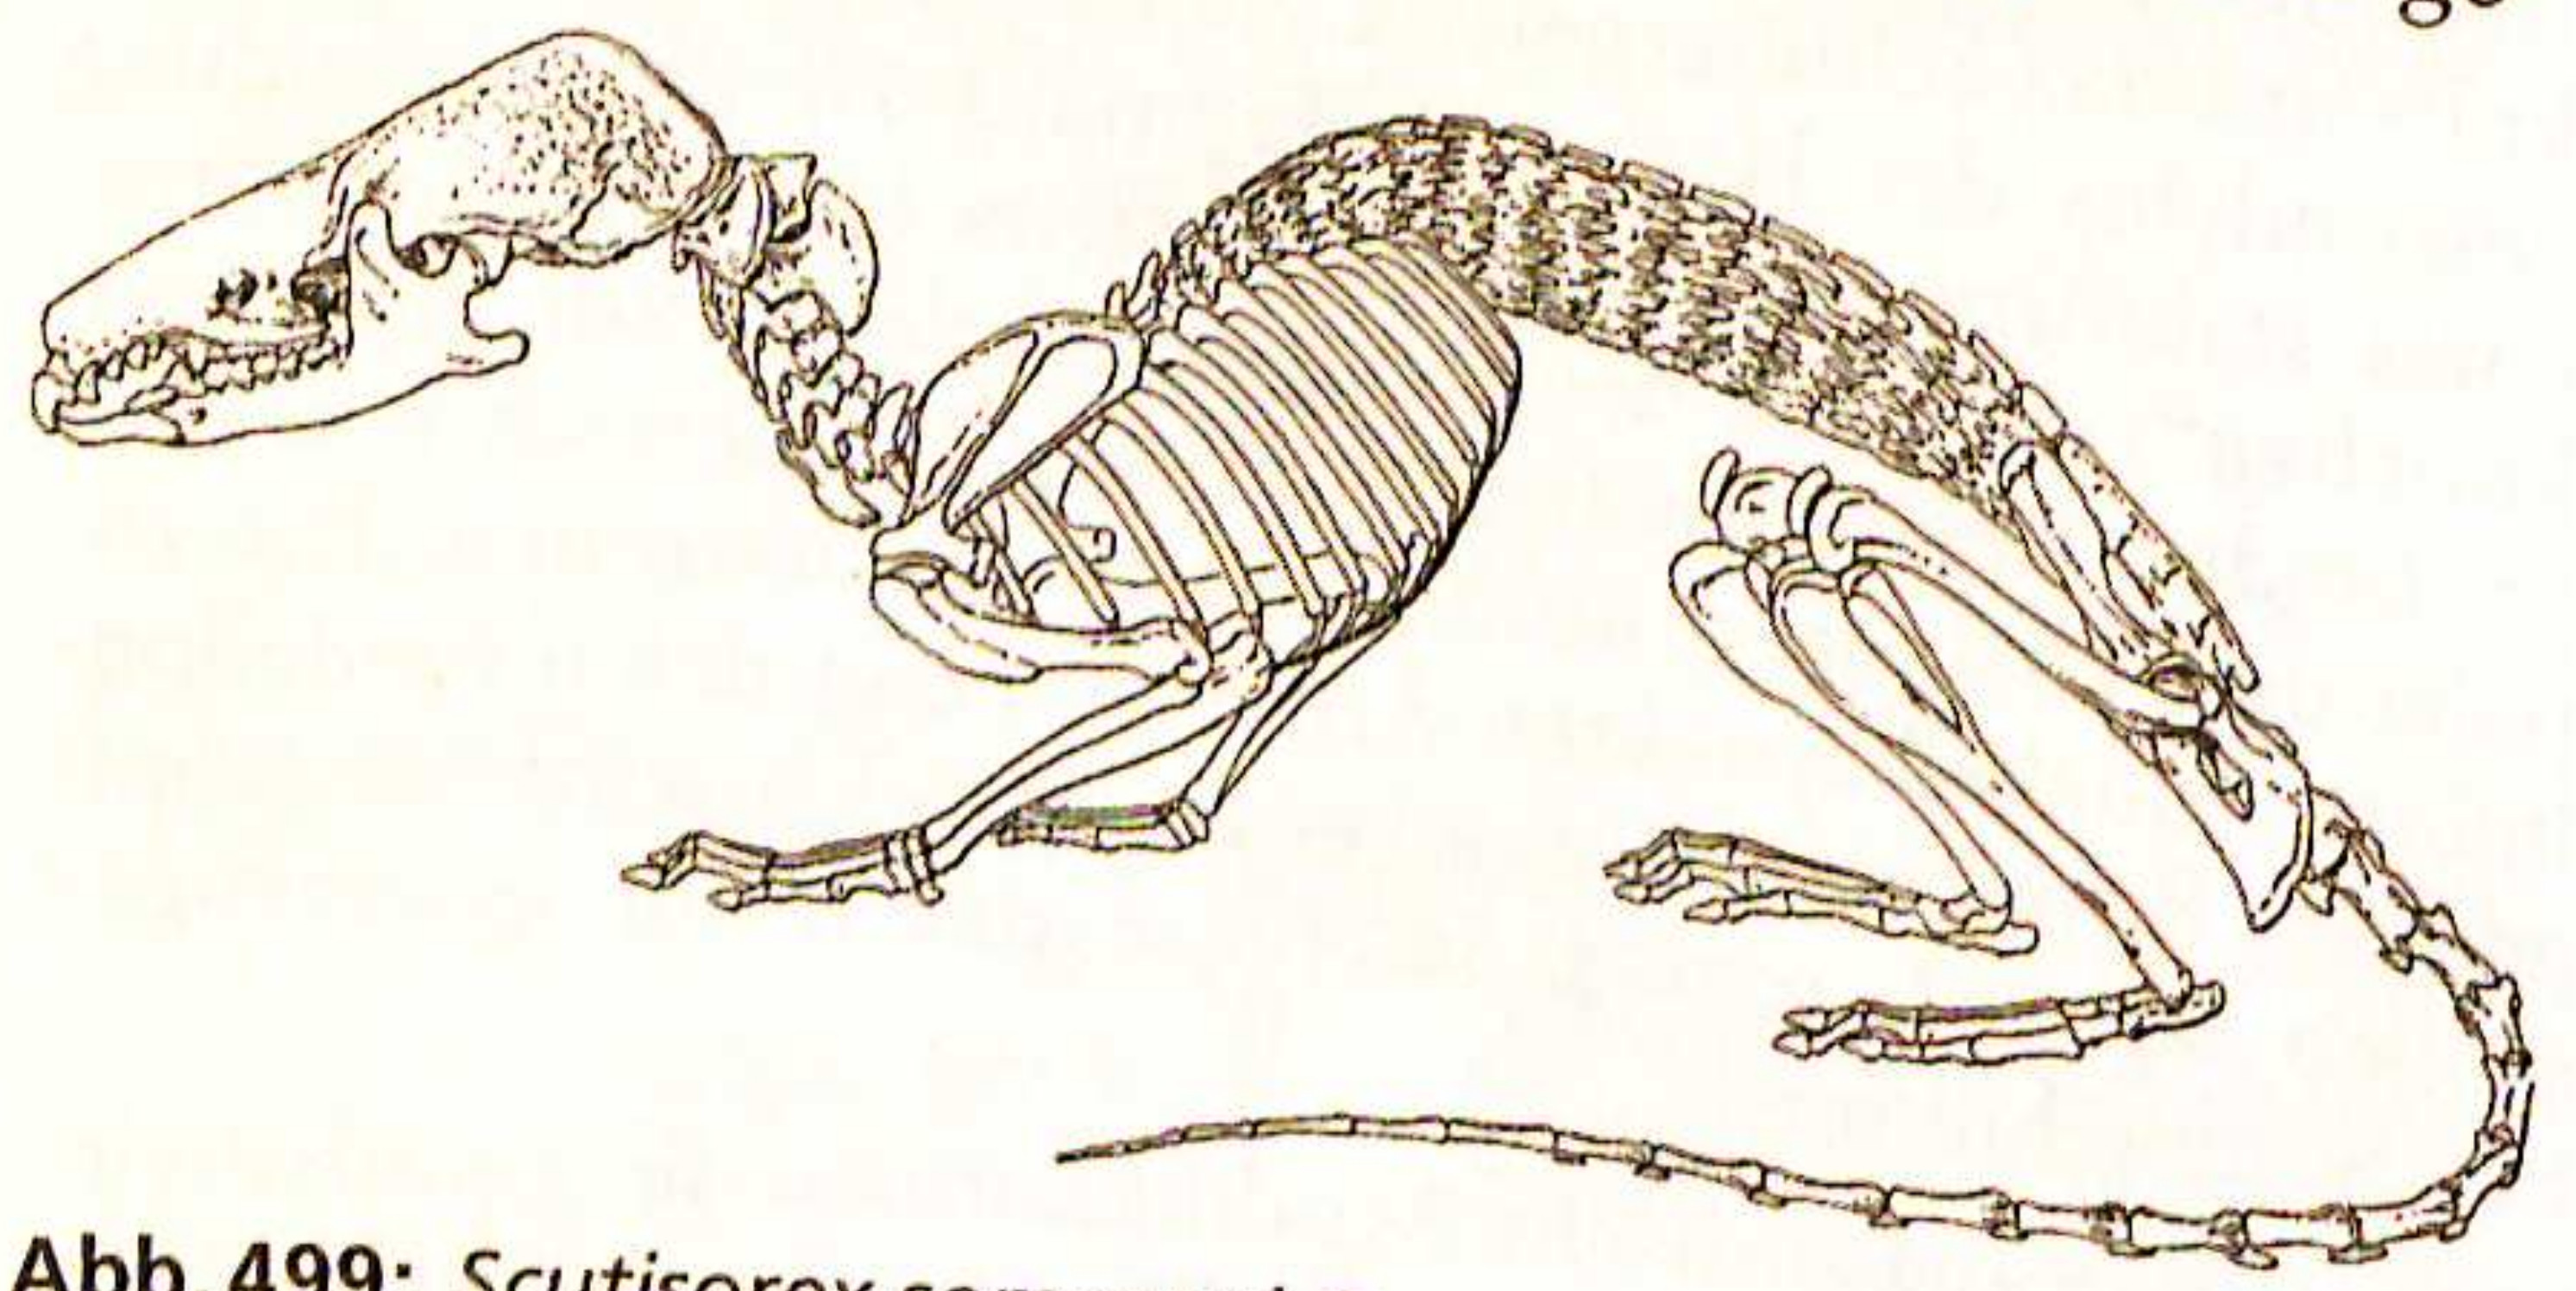
\includegraphics[width=0.2\textwidth]{../PCA/Skelettbilder_klein/Panzerspitzmaus.jpg}}~
\subfloat[Parasaurolophus walkeri]{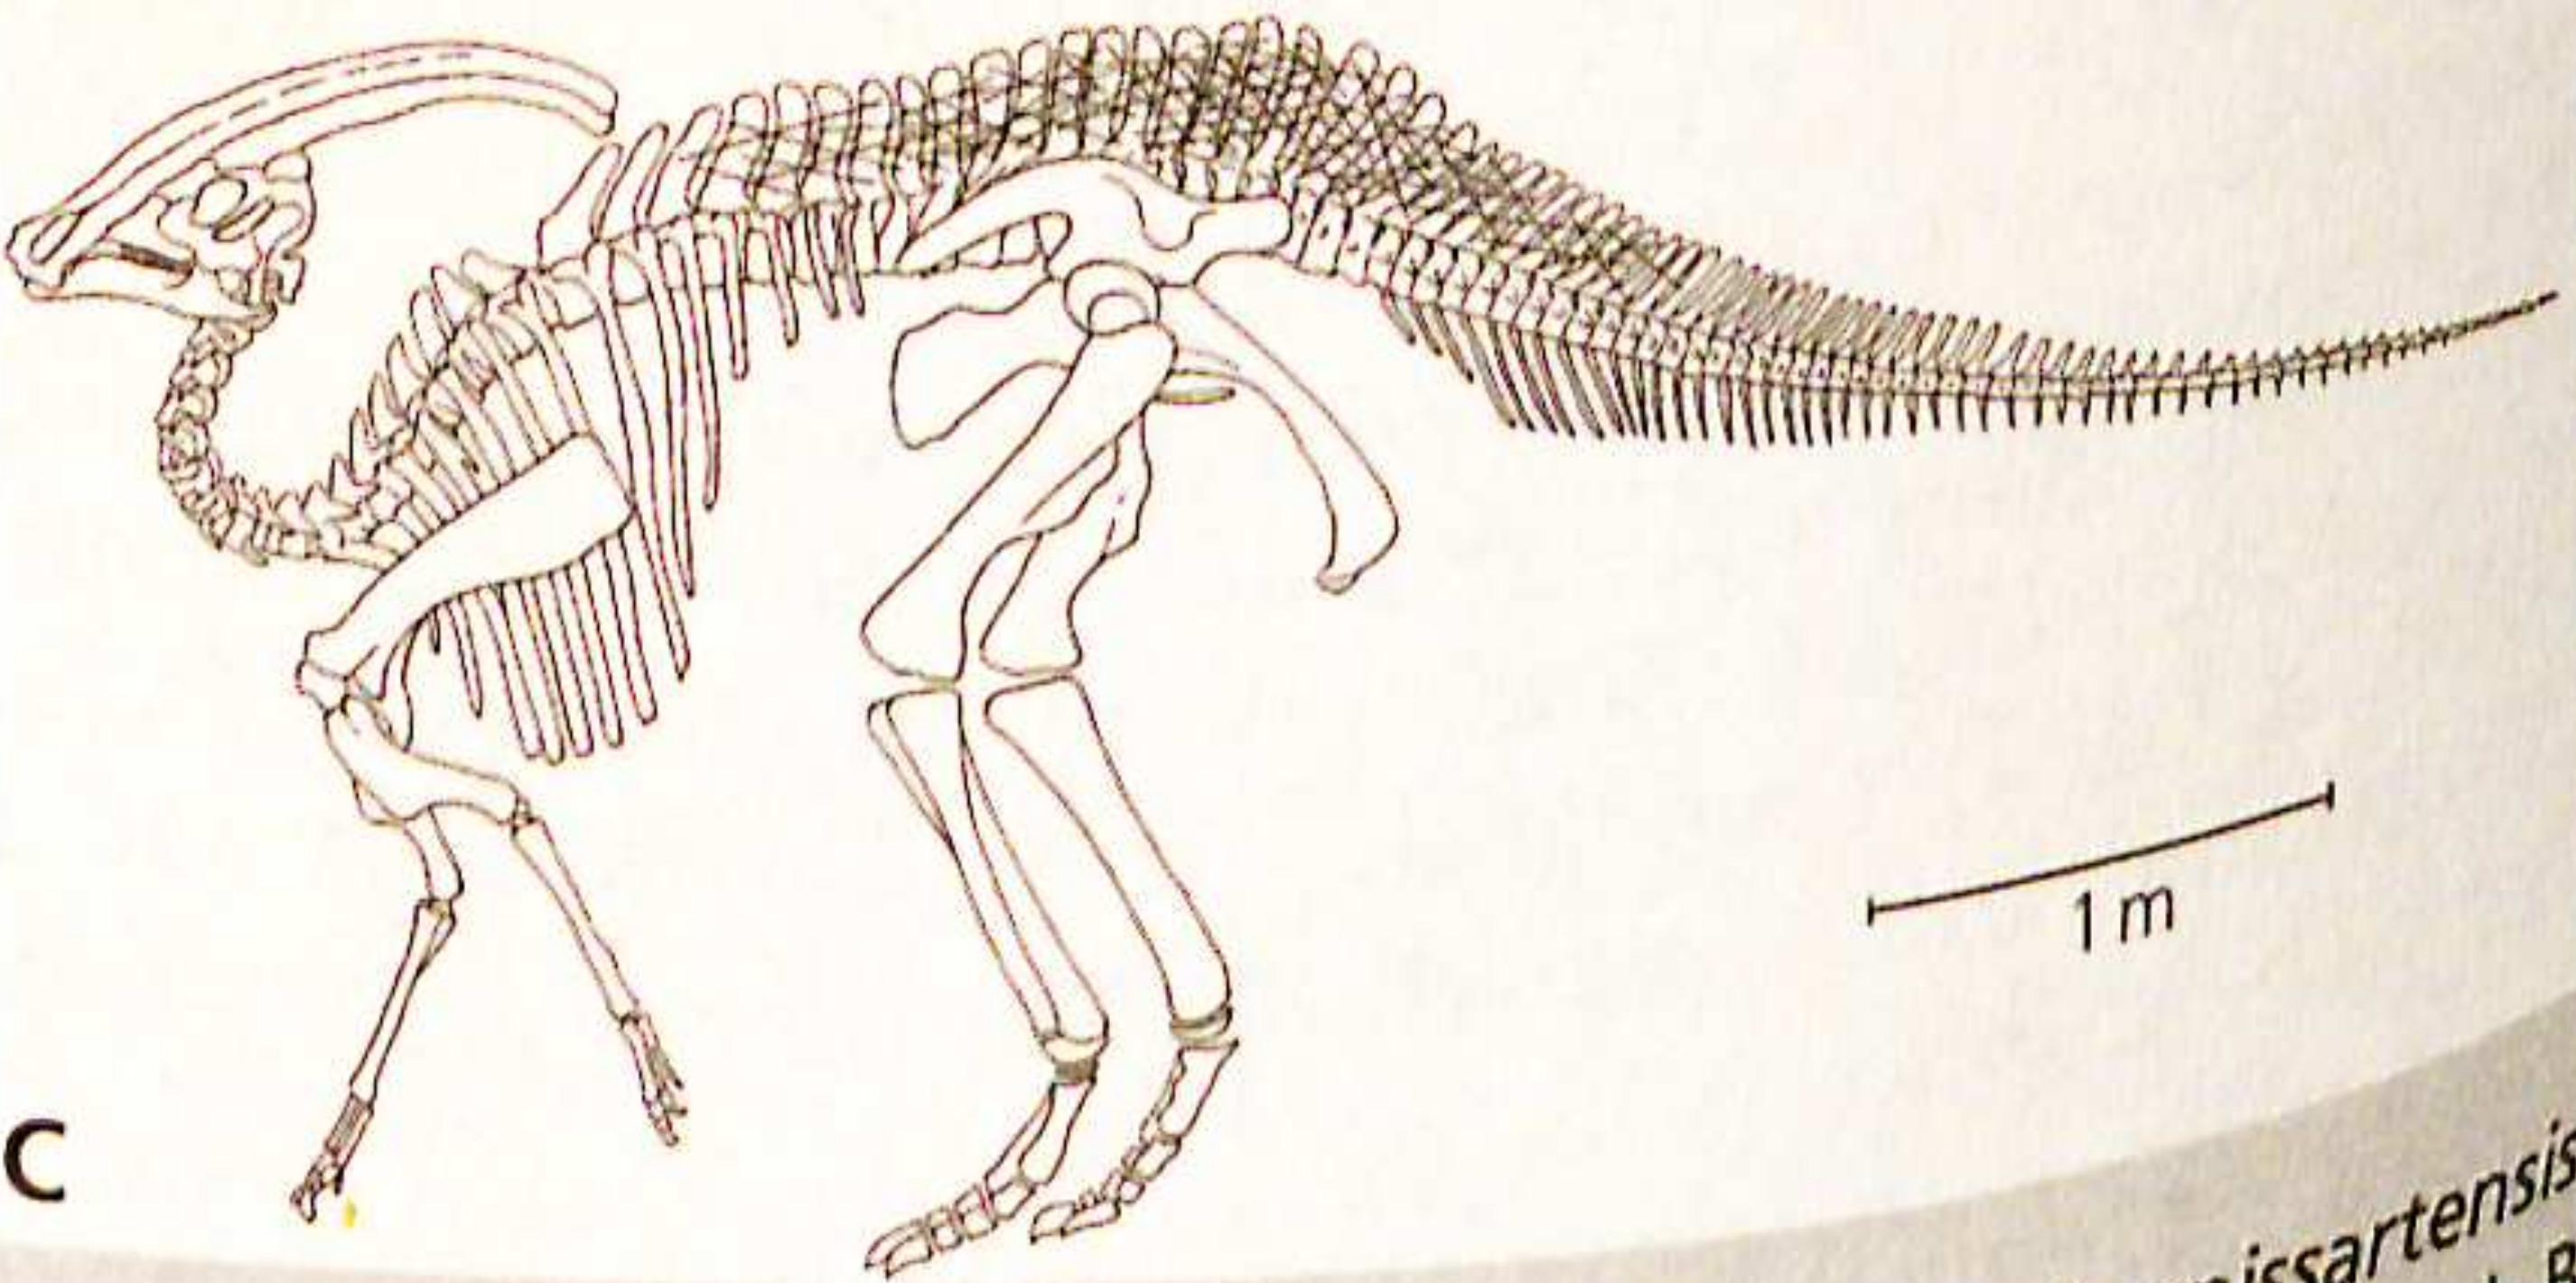
\includegraphics[width=0.2\textwidth]{../PCA/Skelettbilder_klein/Parasaurolophus_walkeri.jpg}}~
\subfloat[Peloneustes philarchus]{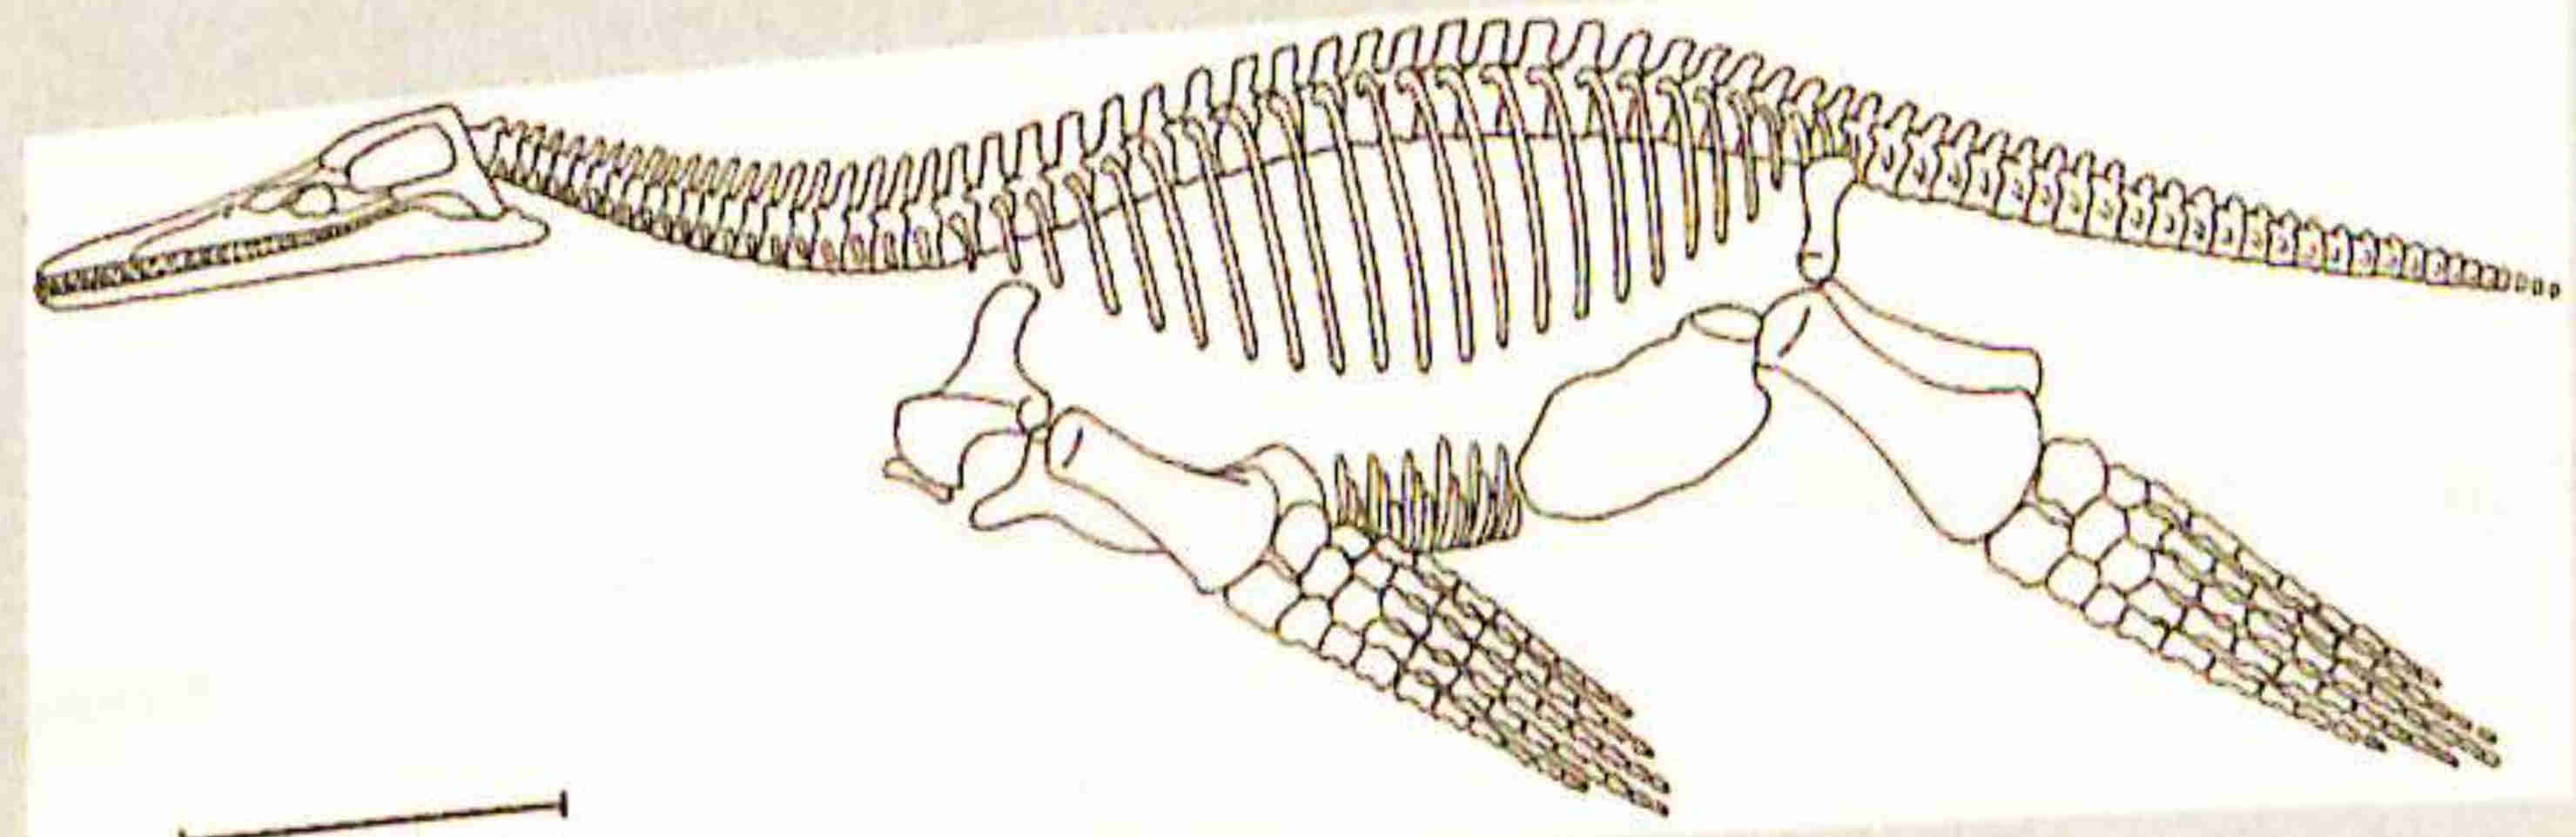
\includegraphics[width=0.2\textwidth]{../PCA/Skelettbilder_klein/Peloneustes_philarchus.jpg}}~
\subfloat[Pferd]{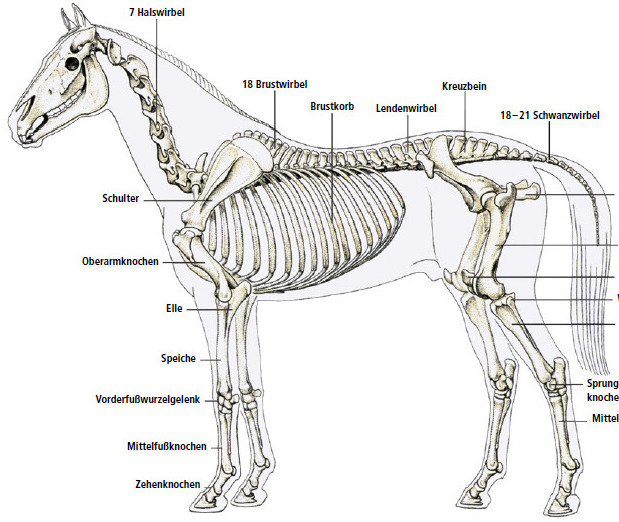
\includegraphics[width=0.2\textwidth]{../PCA/Skelettbilder_klein/Pferd.jpg}}
\\
\subfloat[Pottwal]{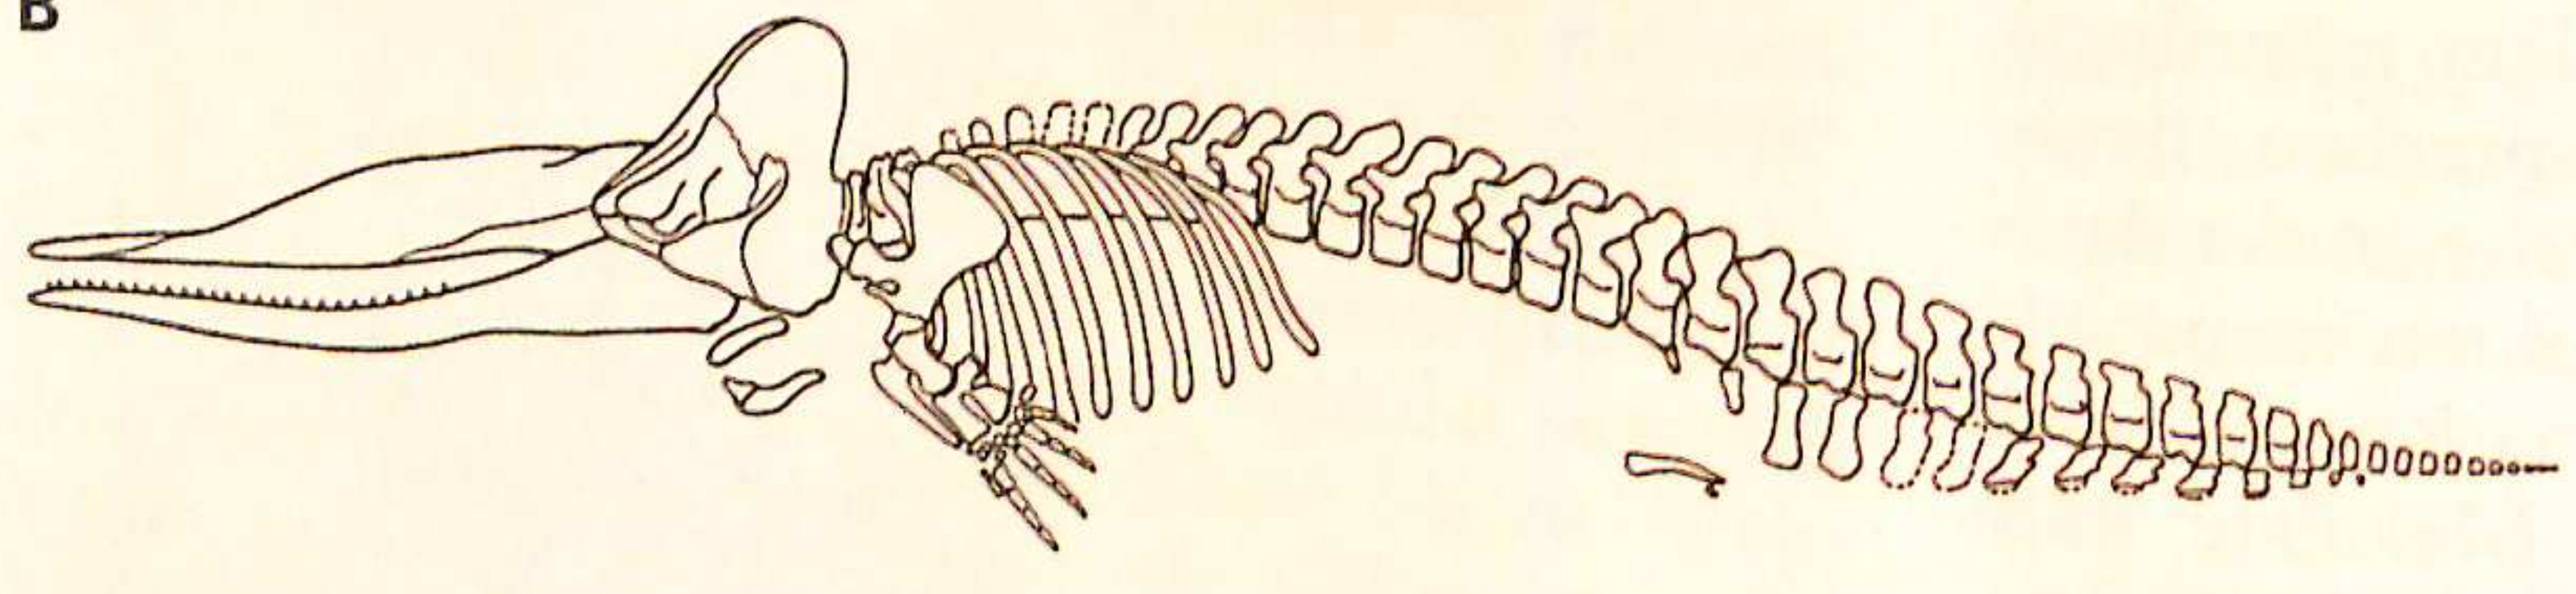
\includegraphics[width=0.2\textwidth]{../PCA/Skelettbilder_klein/Pottwal.jpg}}~
\subfloat[Rothirsch]{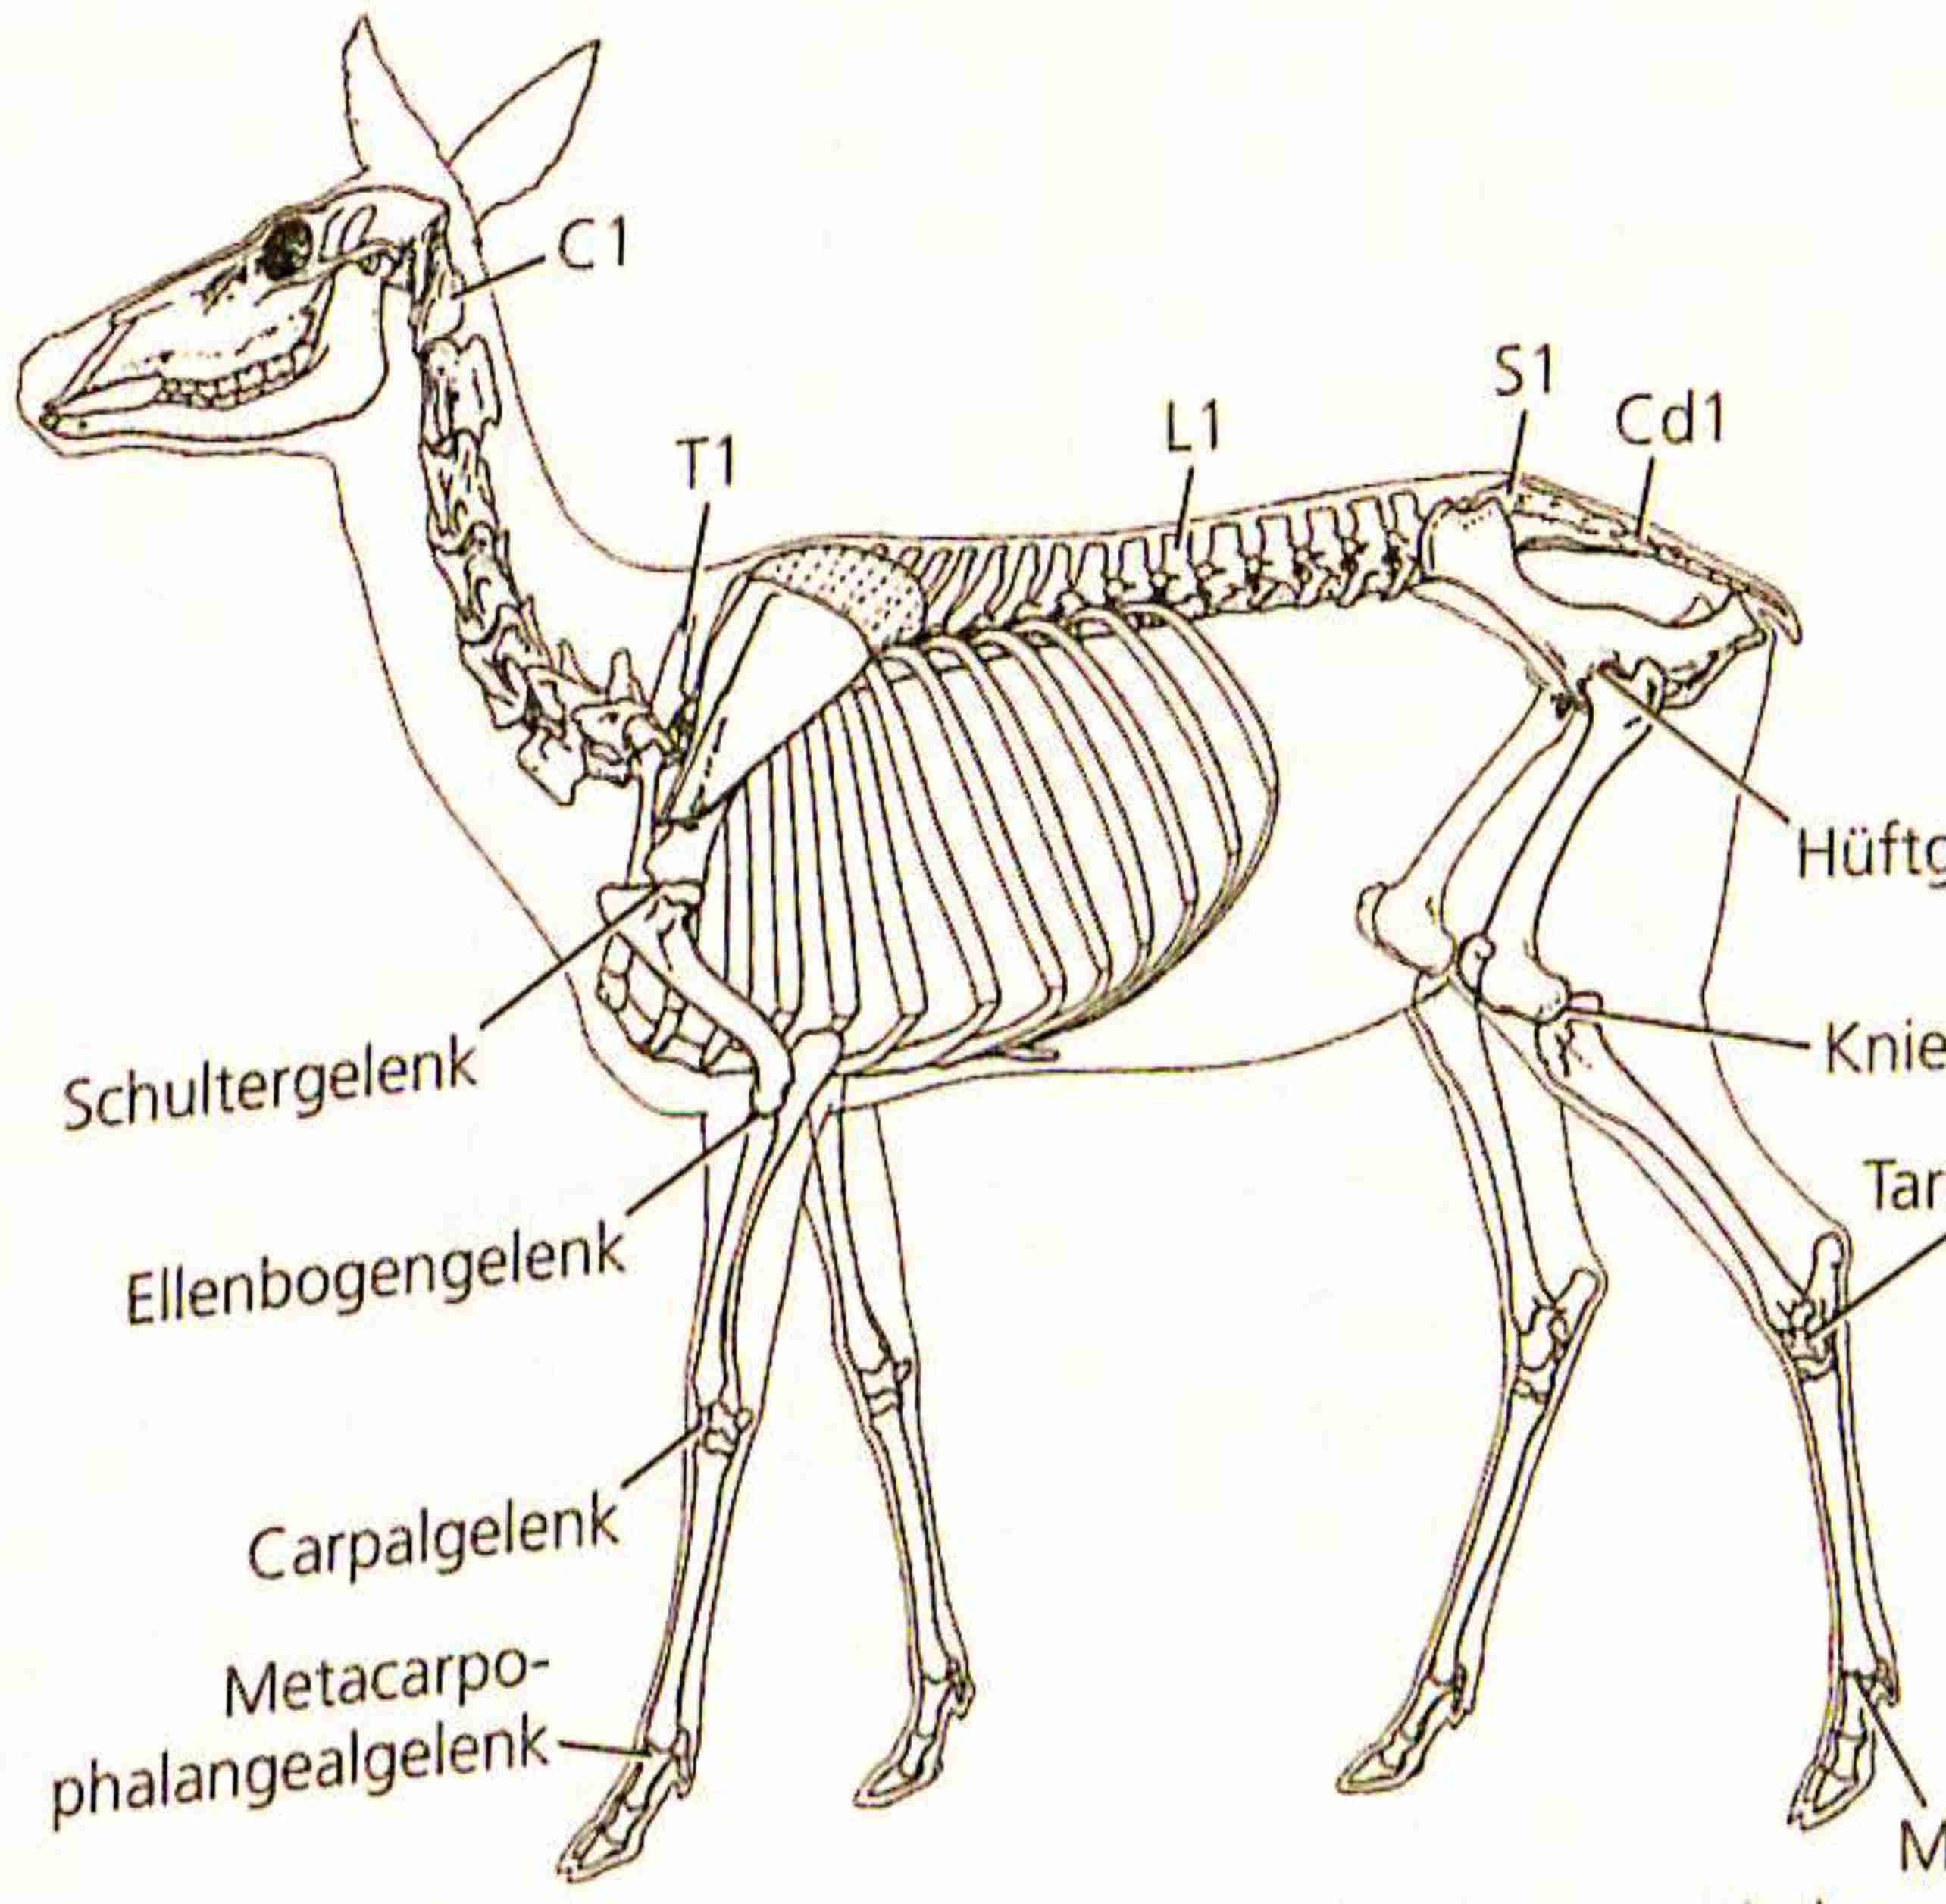
\includegraphics[width=0.2\textwidth]{../PCA/Skelettbilder_klein/Rothirsch.jpg}}~
\subfloat[Schwan]{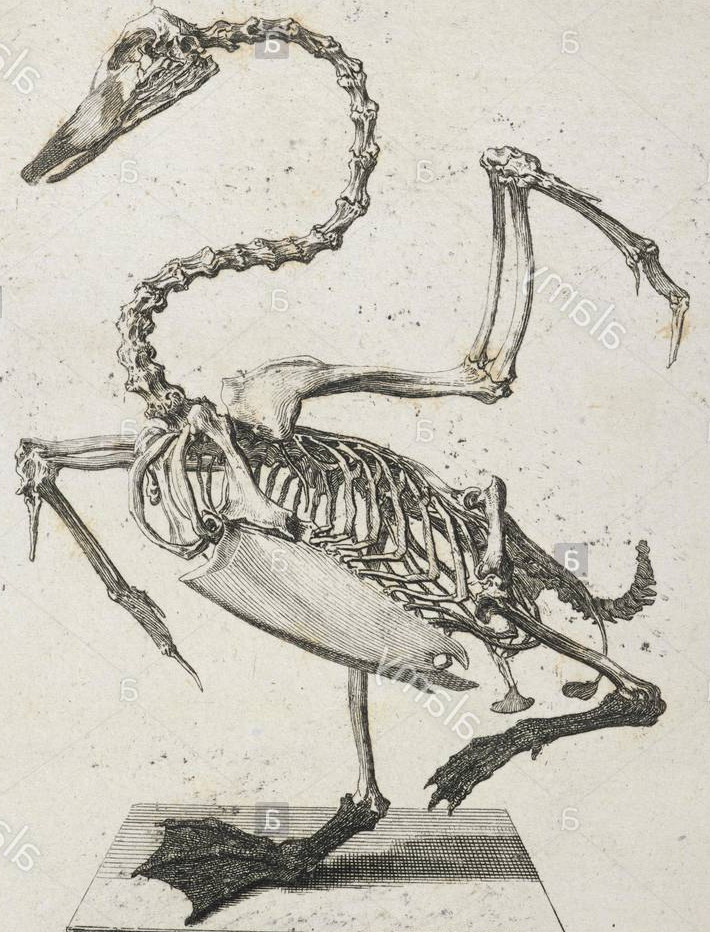
\includegraphics[width=0.2\textwidth]{../PCA/Skelettbilder_klein/Schwan.jpg}}~
\subfloat[Schwein]{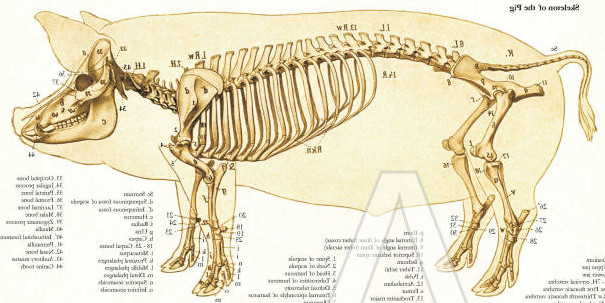
\includegraphics[width=0.2\textwidth]{../PCA/Skelettbilder_klein/Schwein.jpg}}~
\subfloat[Seehund]{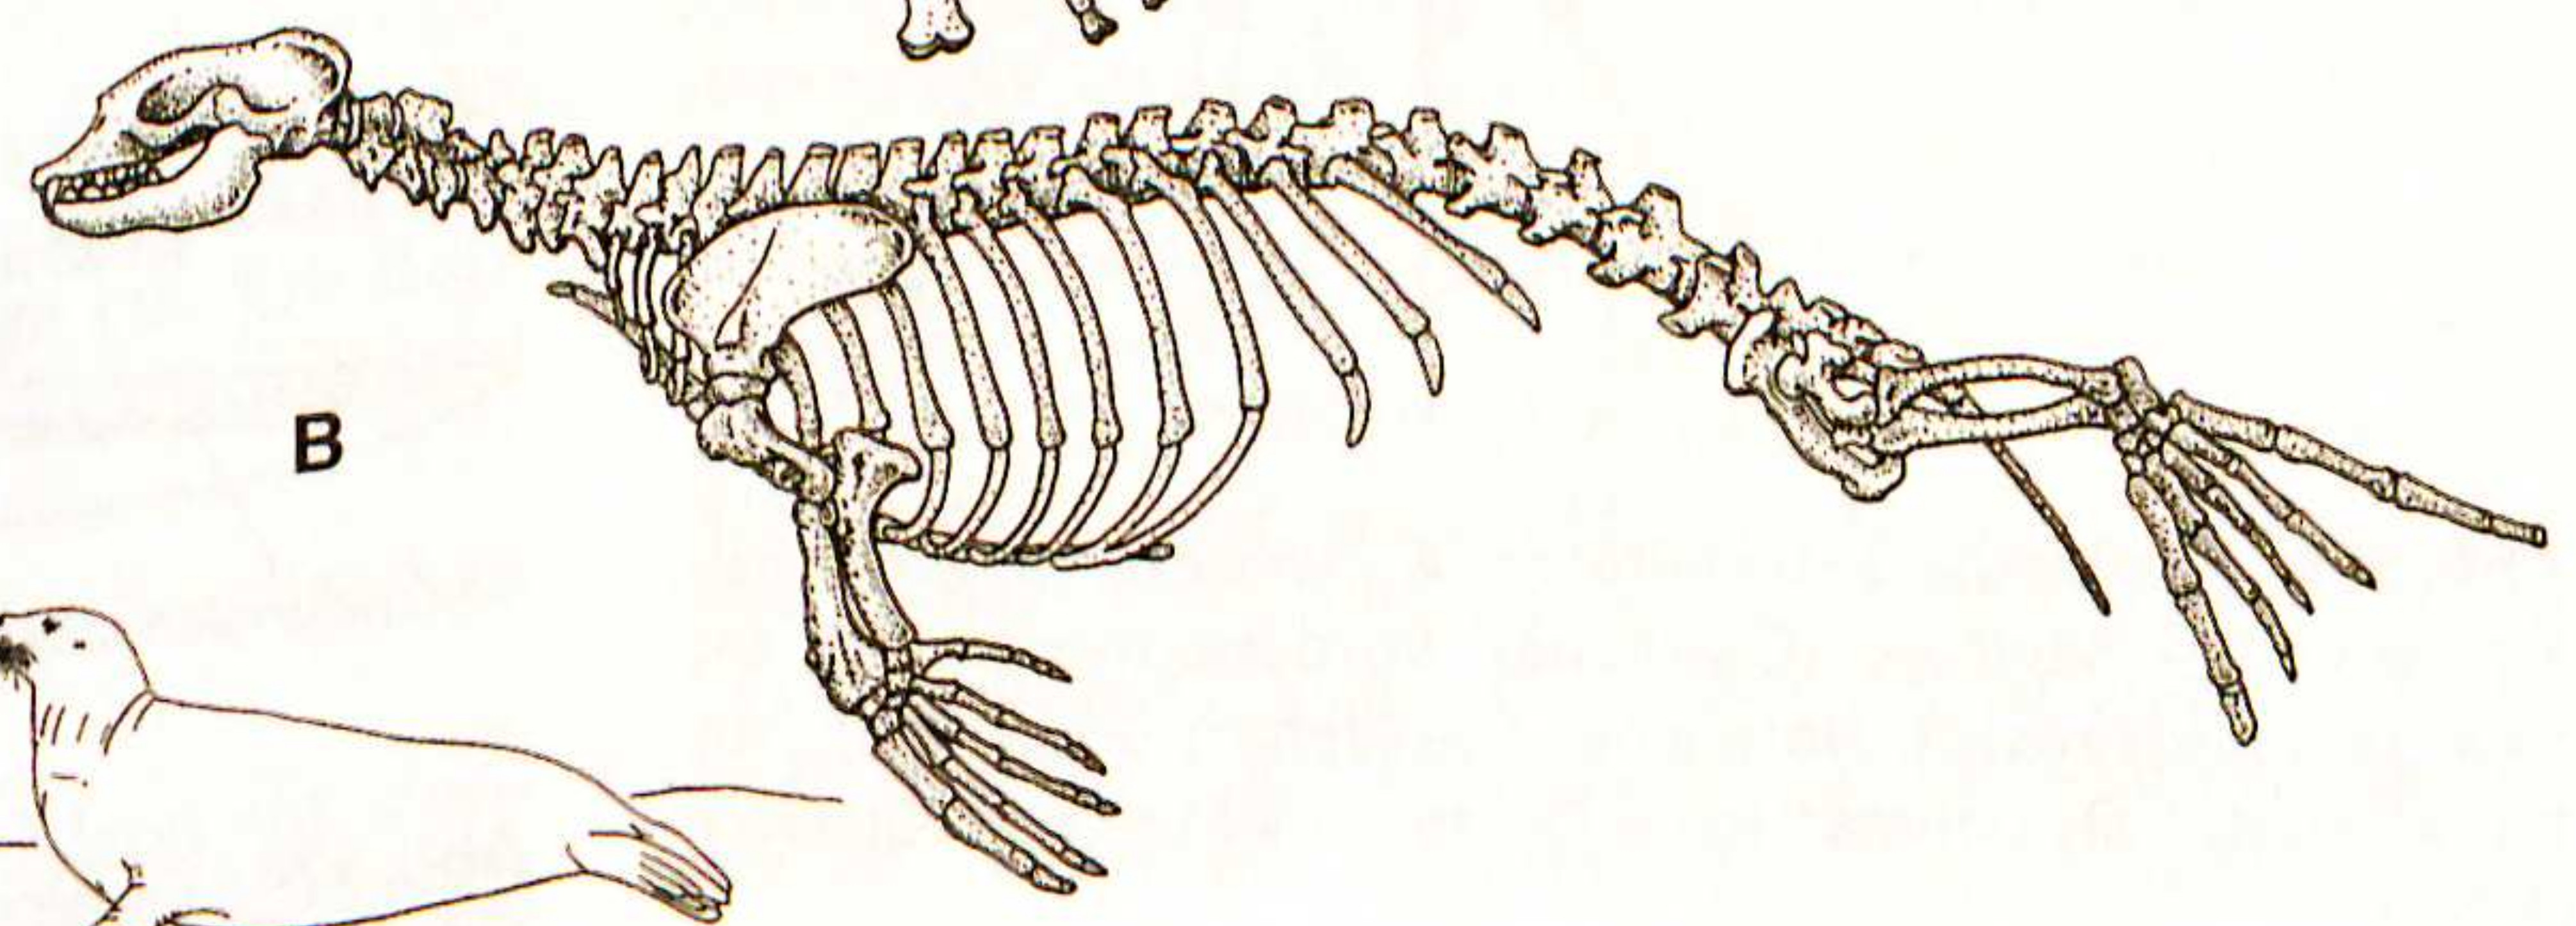
\includegraphics[width=0.2\textwidth]{../PCA/Skelettbilder_klein/Seehund.jpg}}
\\
\subfloat[Sinornis]{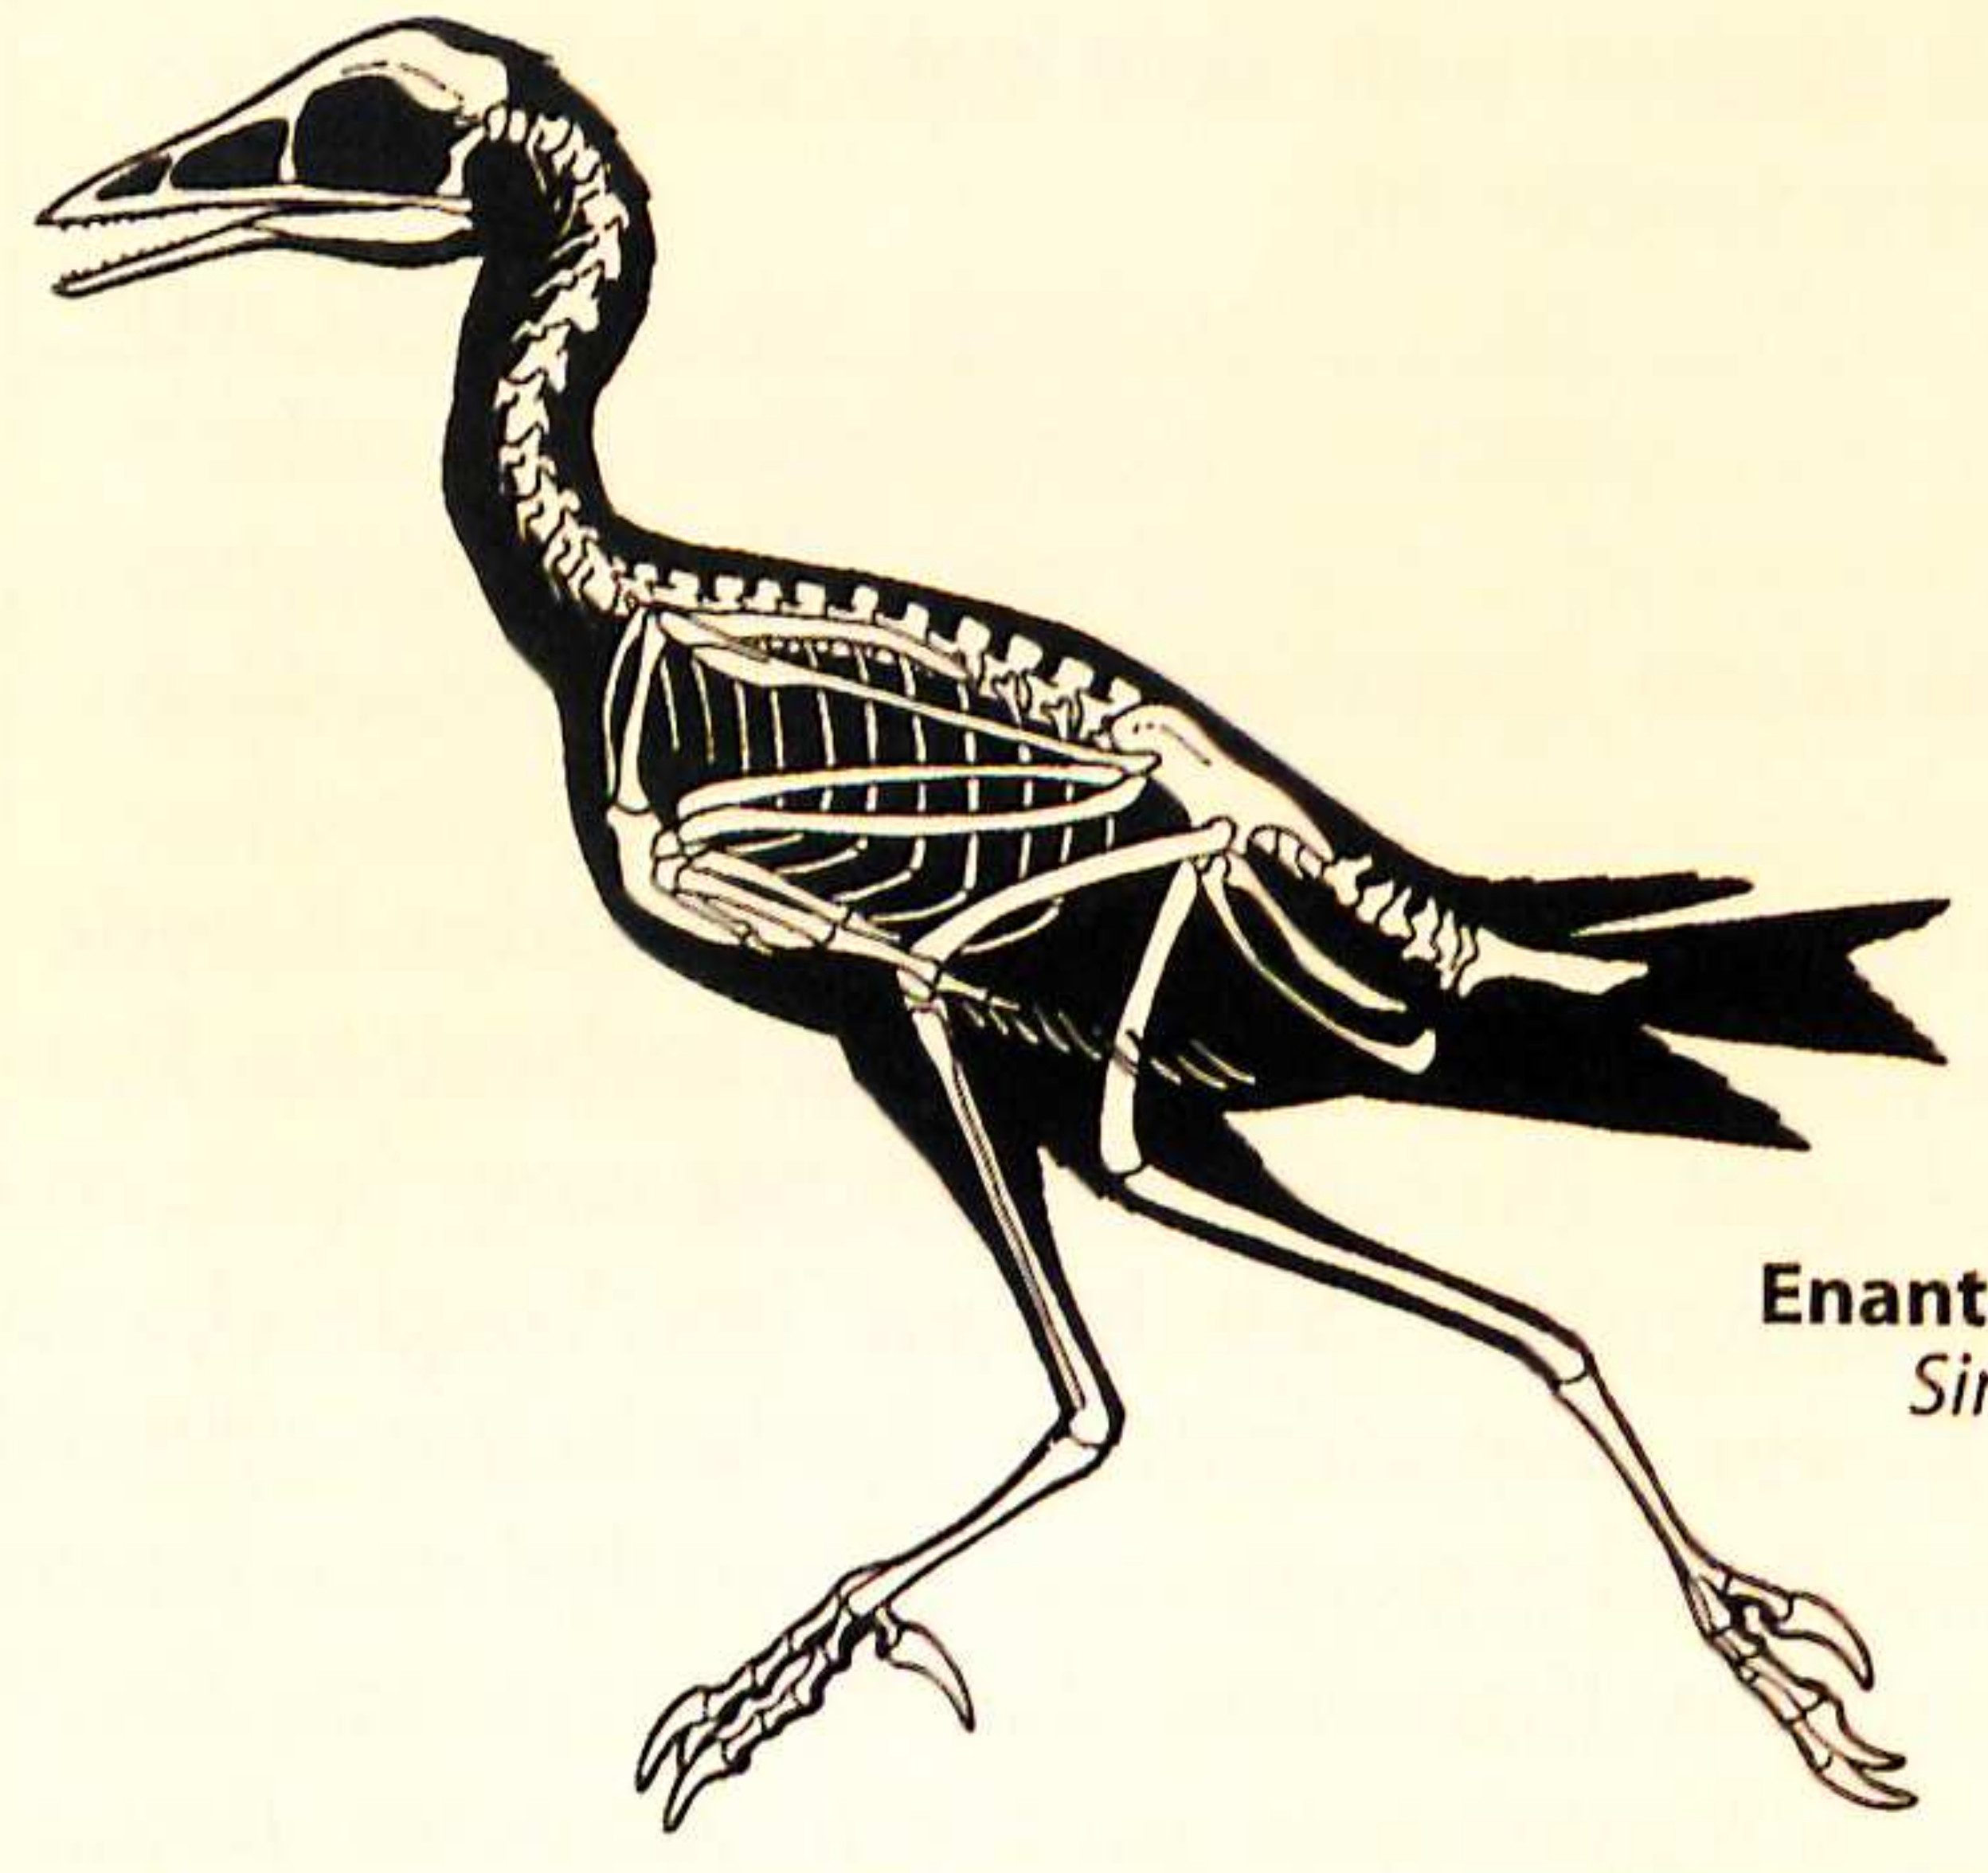
\includegraphics[width=0.2\textwidth]{../PCA/Skelettbilder_klein/Sinornis.jpg}}~
\subfloat[Stegosaurus]{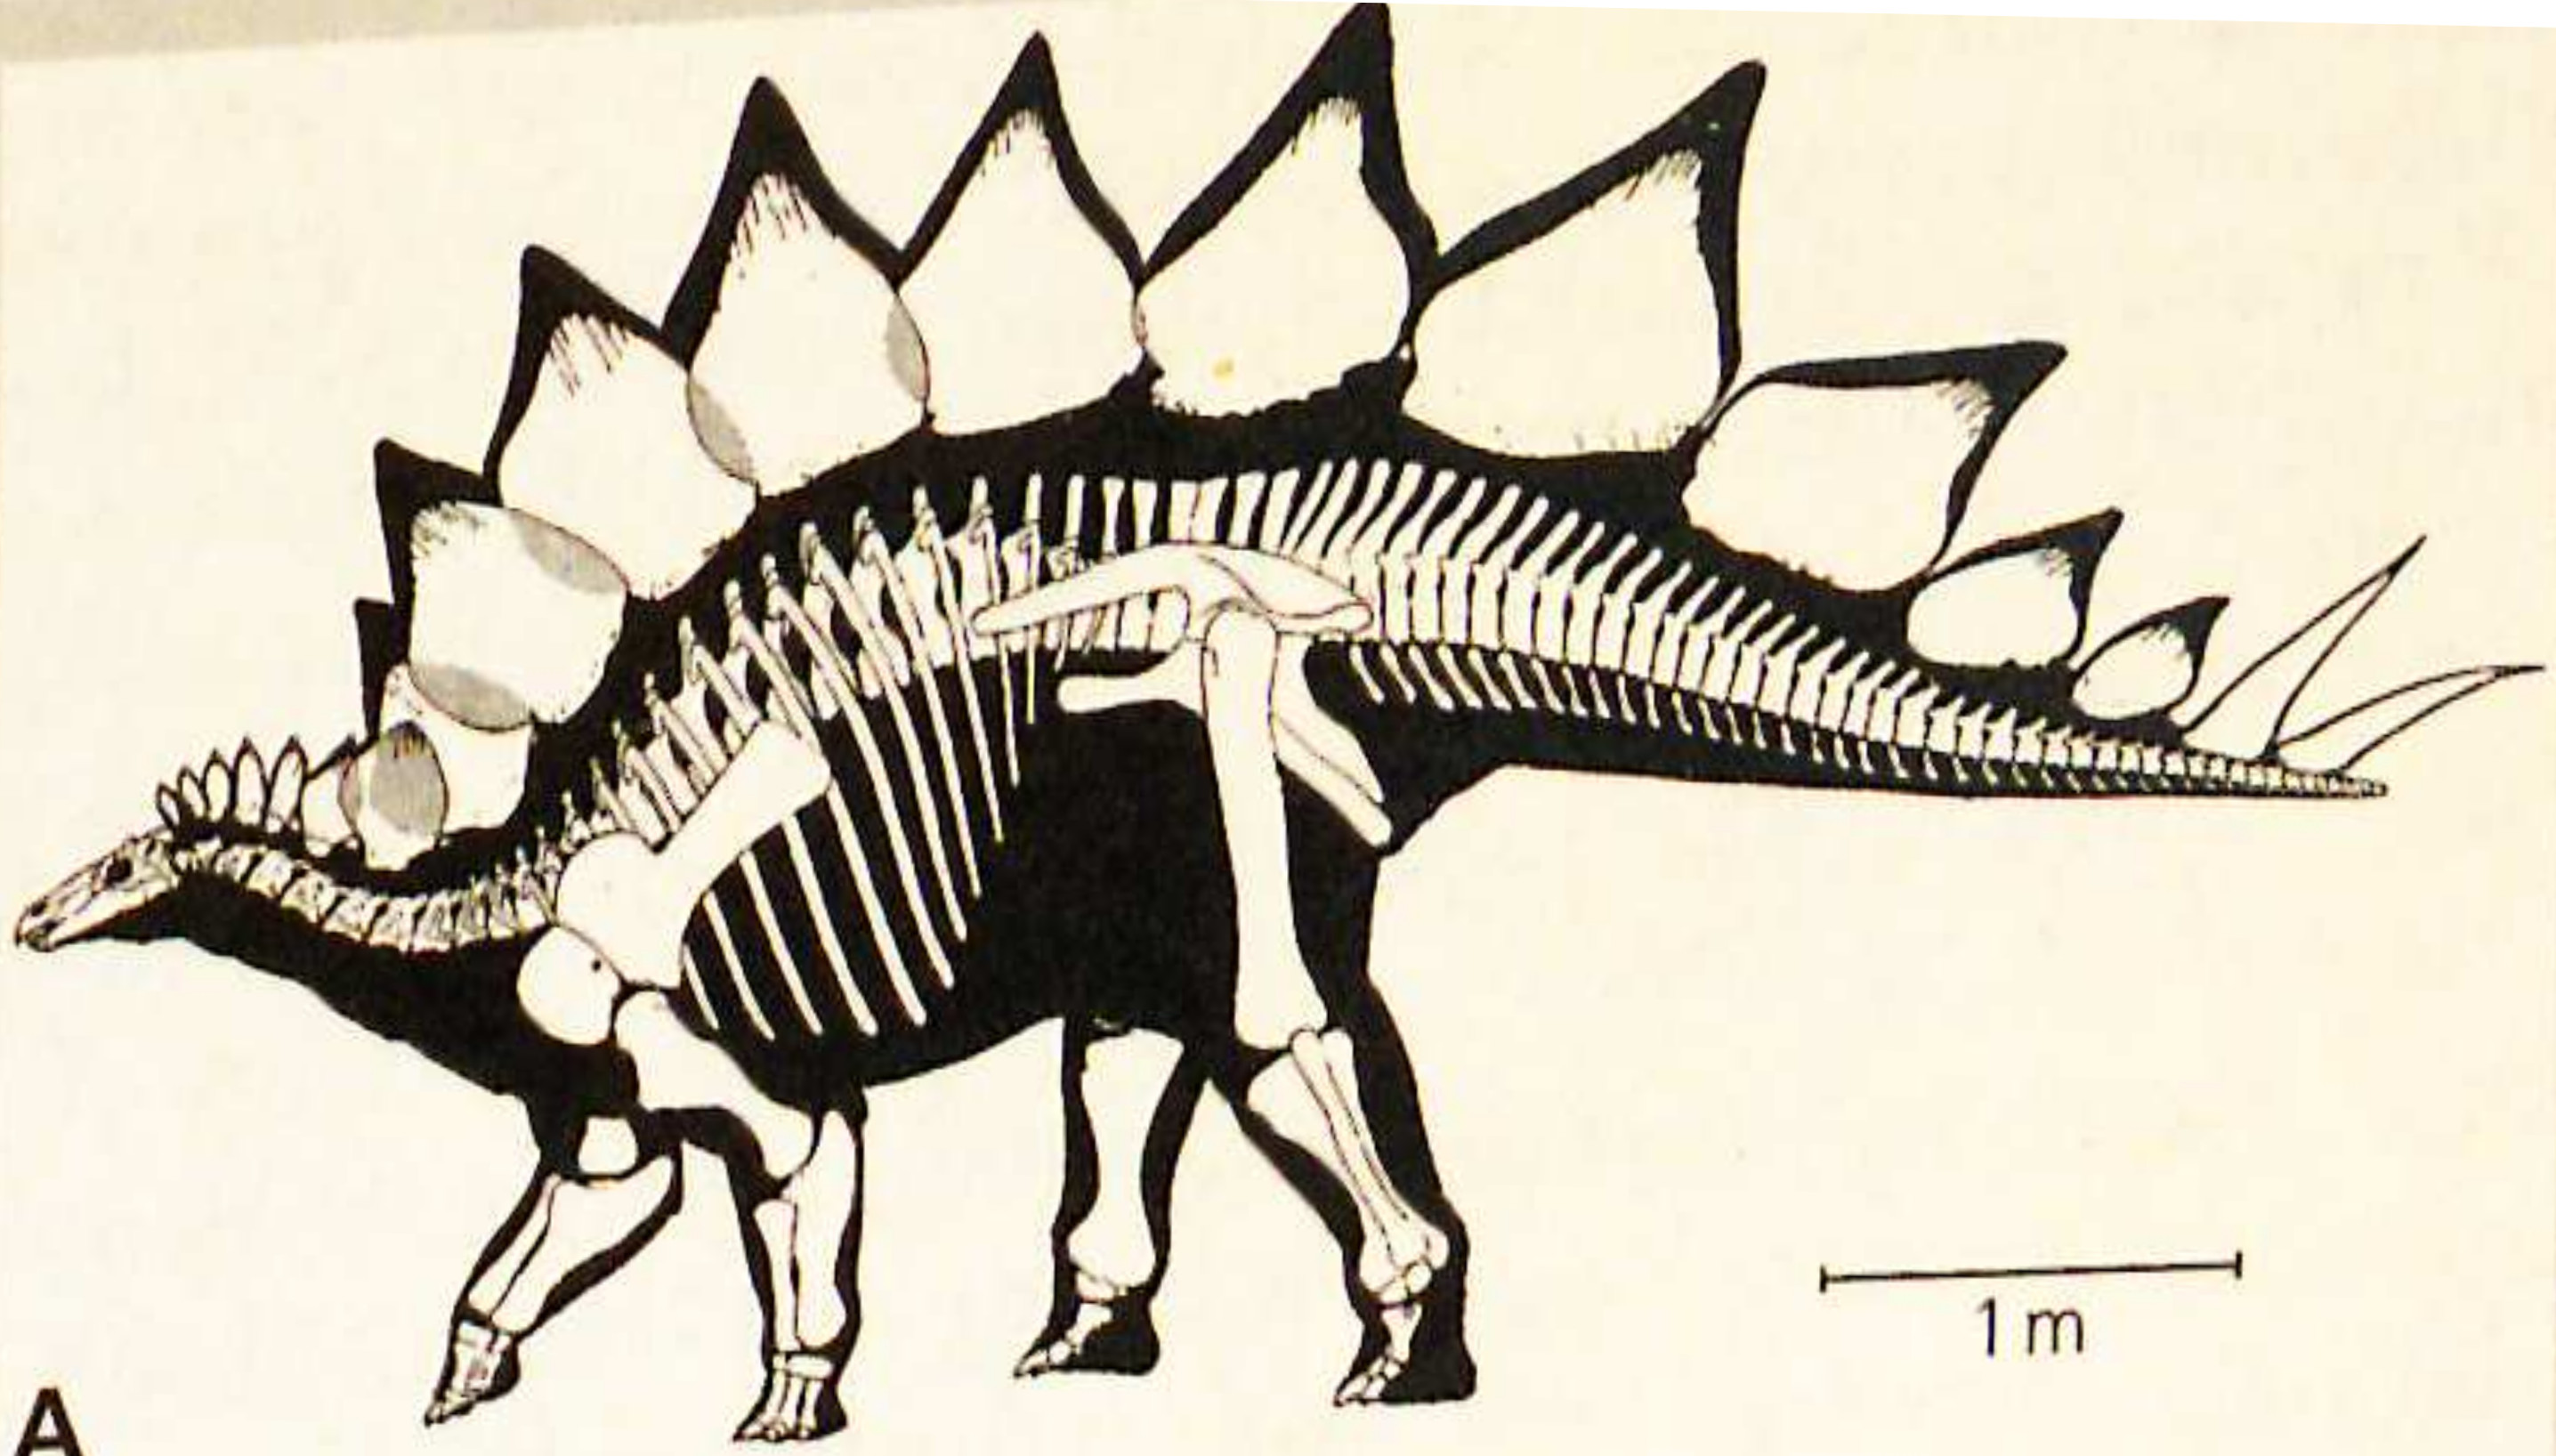
\includegraphics[width=0.2\textwidth]{../PCA/Skelettbilder_klein/Stegosaurus.jpg}}~
\subfloat[Strauss]{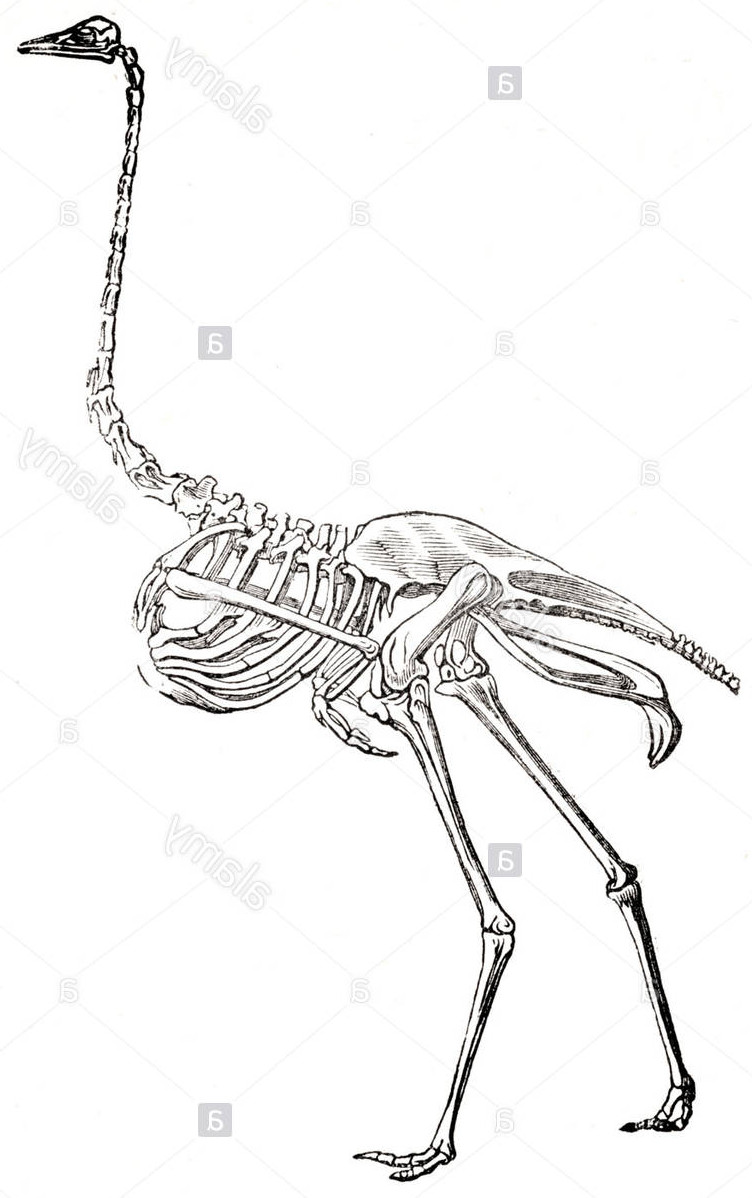
\includegraphics[width=0.2\textwidth]{../PCA/Skelettbilder_klein/Strauss.jpg}}~
\subfloat[Taube]{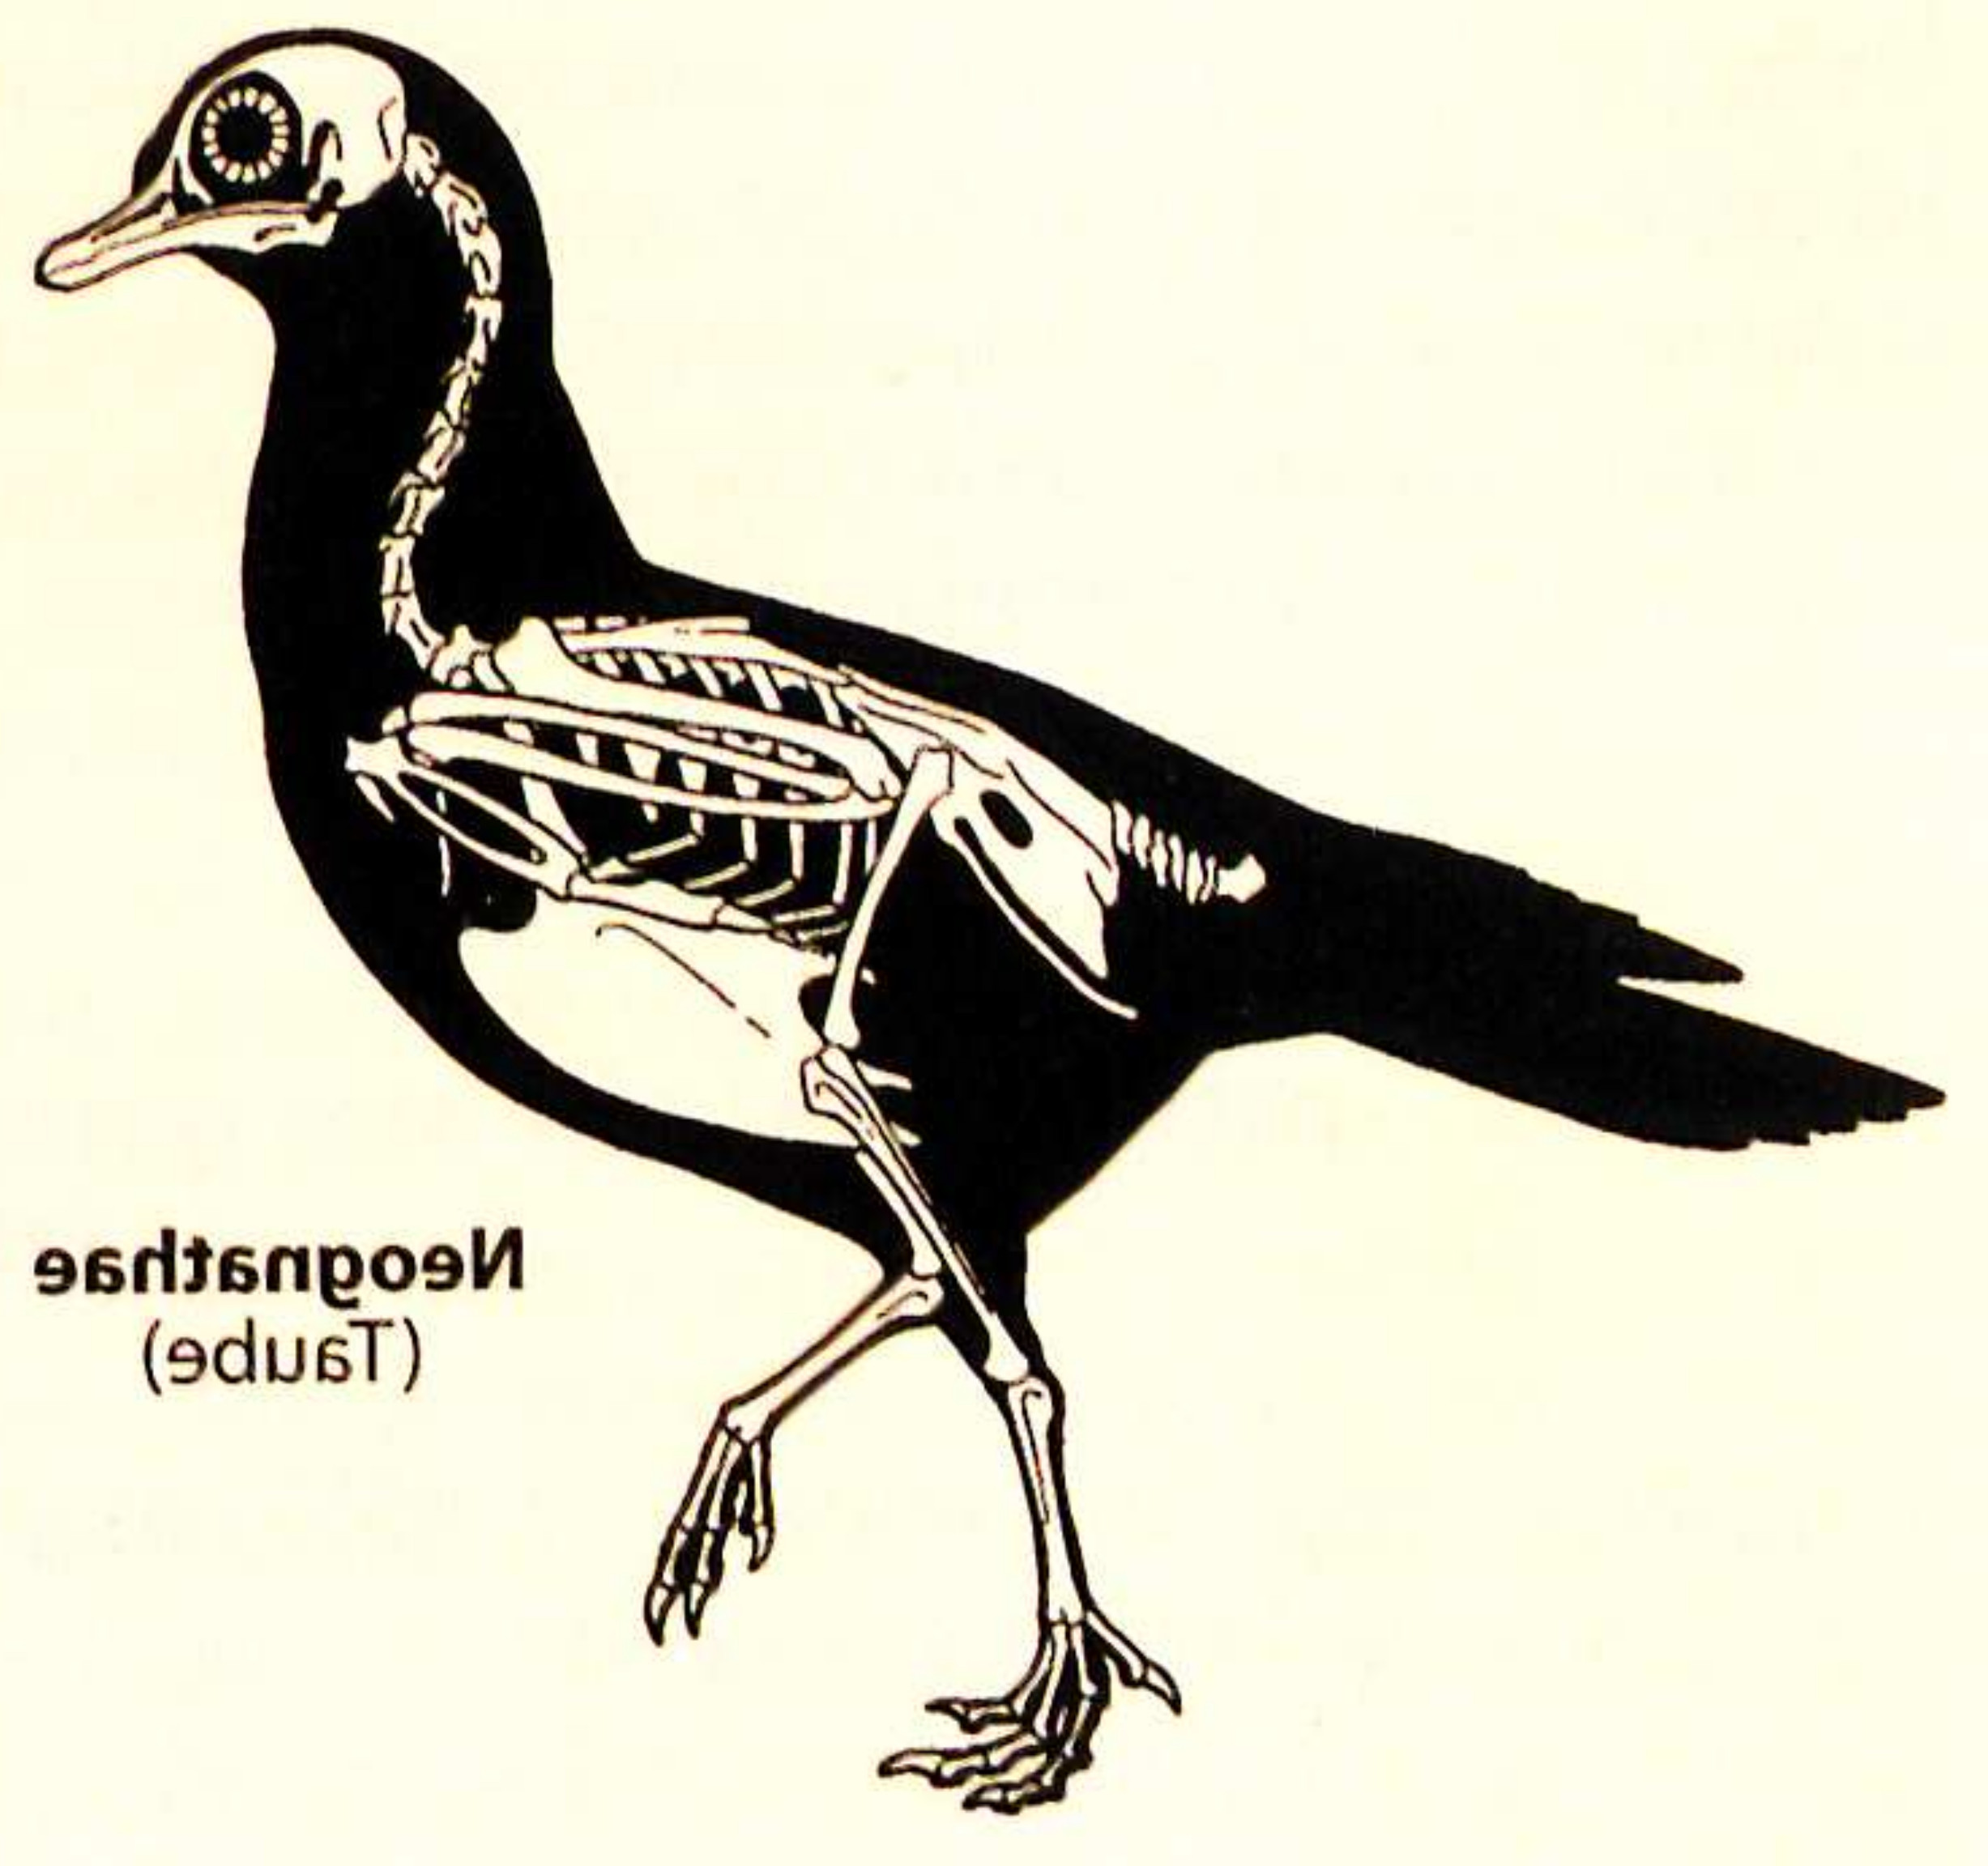
\includegraphics[width=0.2\textwidth]{../PCA/Skelettbilder_klein/Taube.jpg}}~
\subfloat[Thrinaxodon]{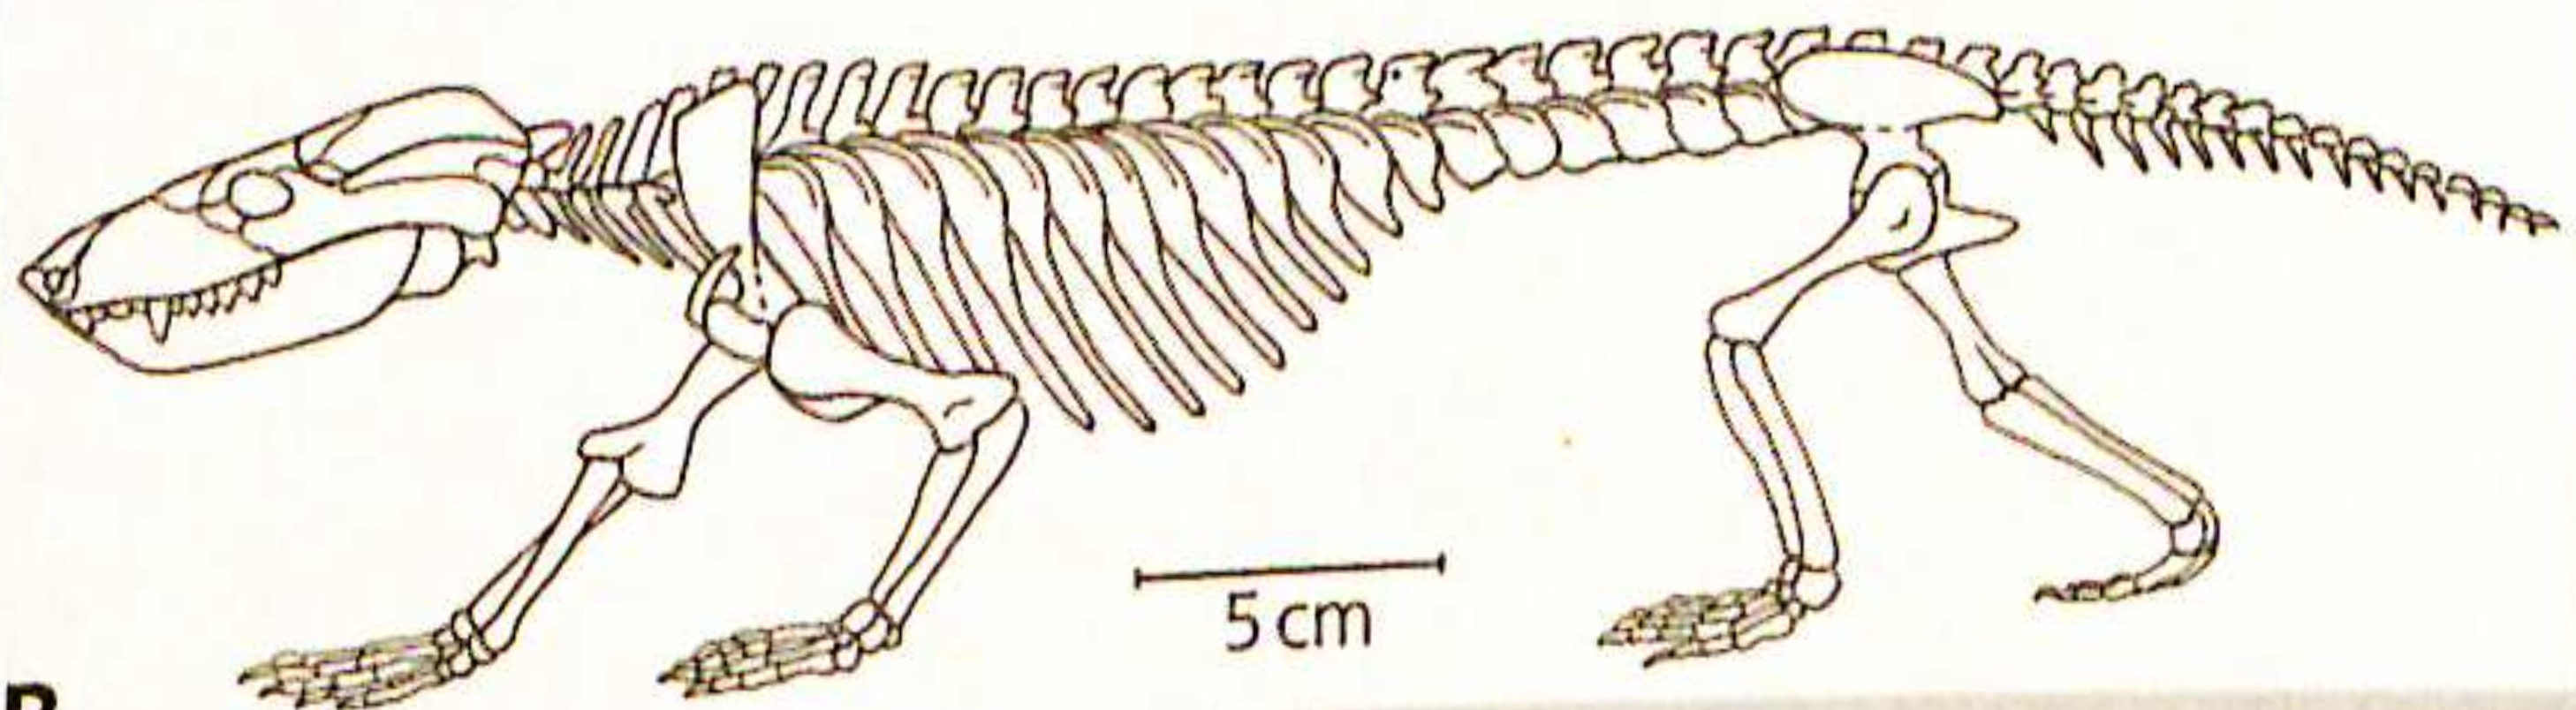
\includegraphics[width=0.2\textwidth]{../PCA/Skelettbilder_klein/Thrinaxodon.jpg}}
\\
\subfloat[Triceratops]{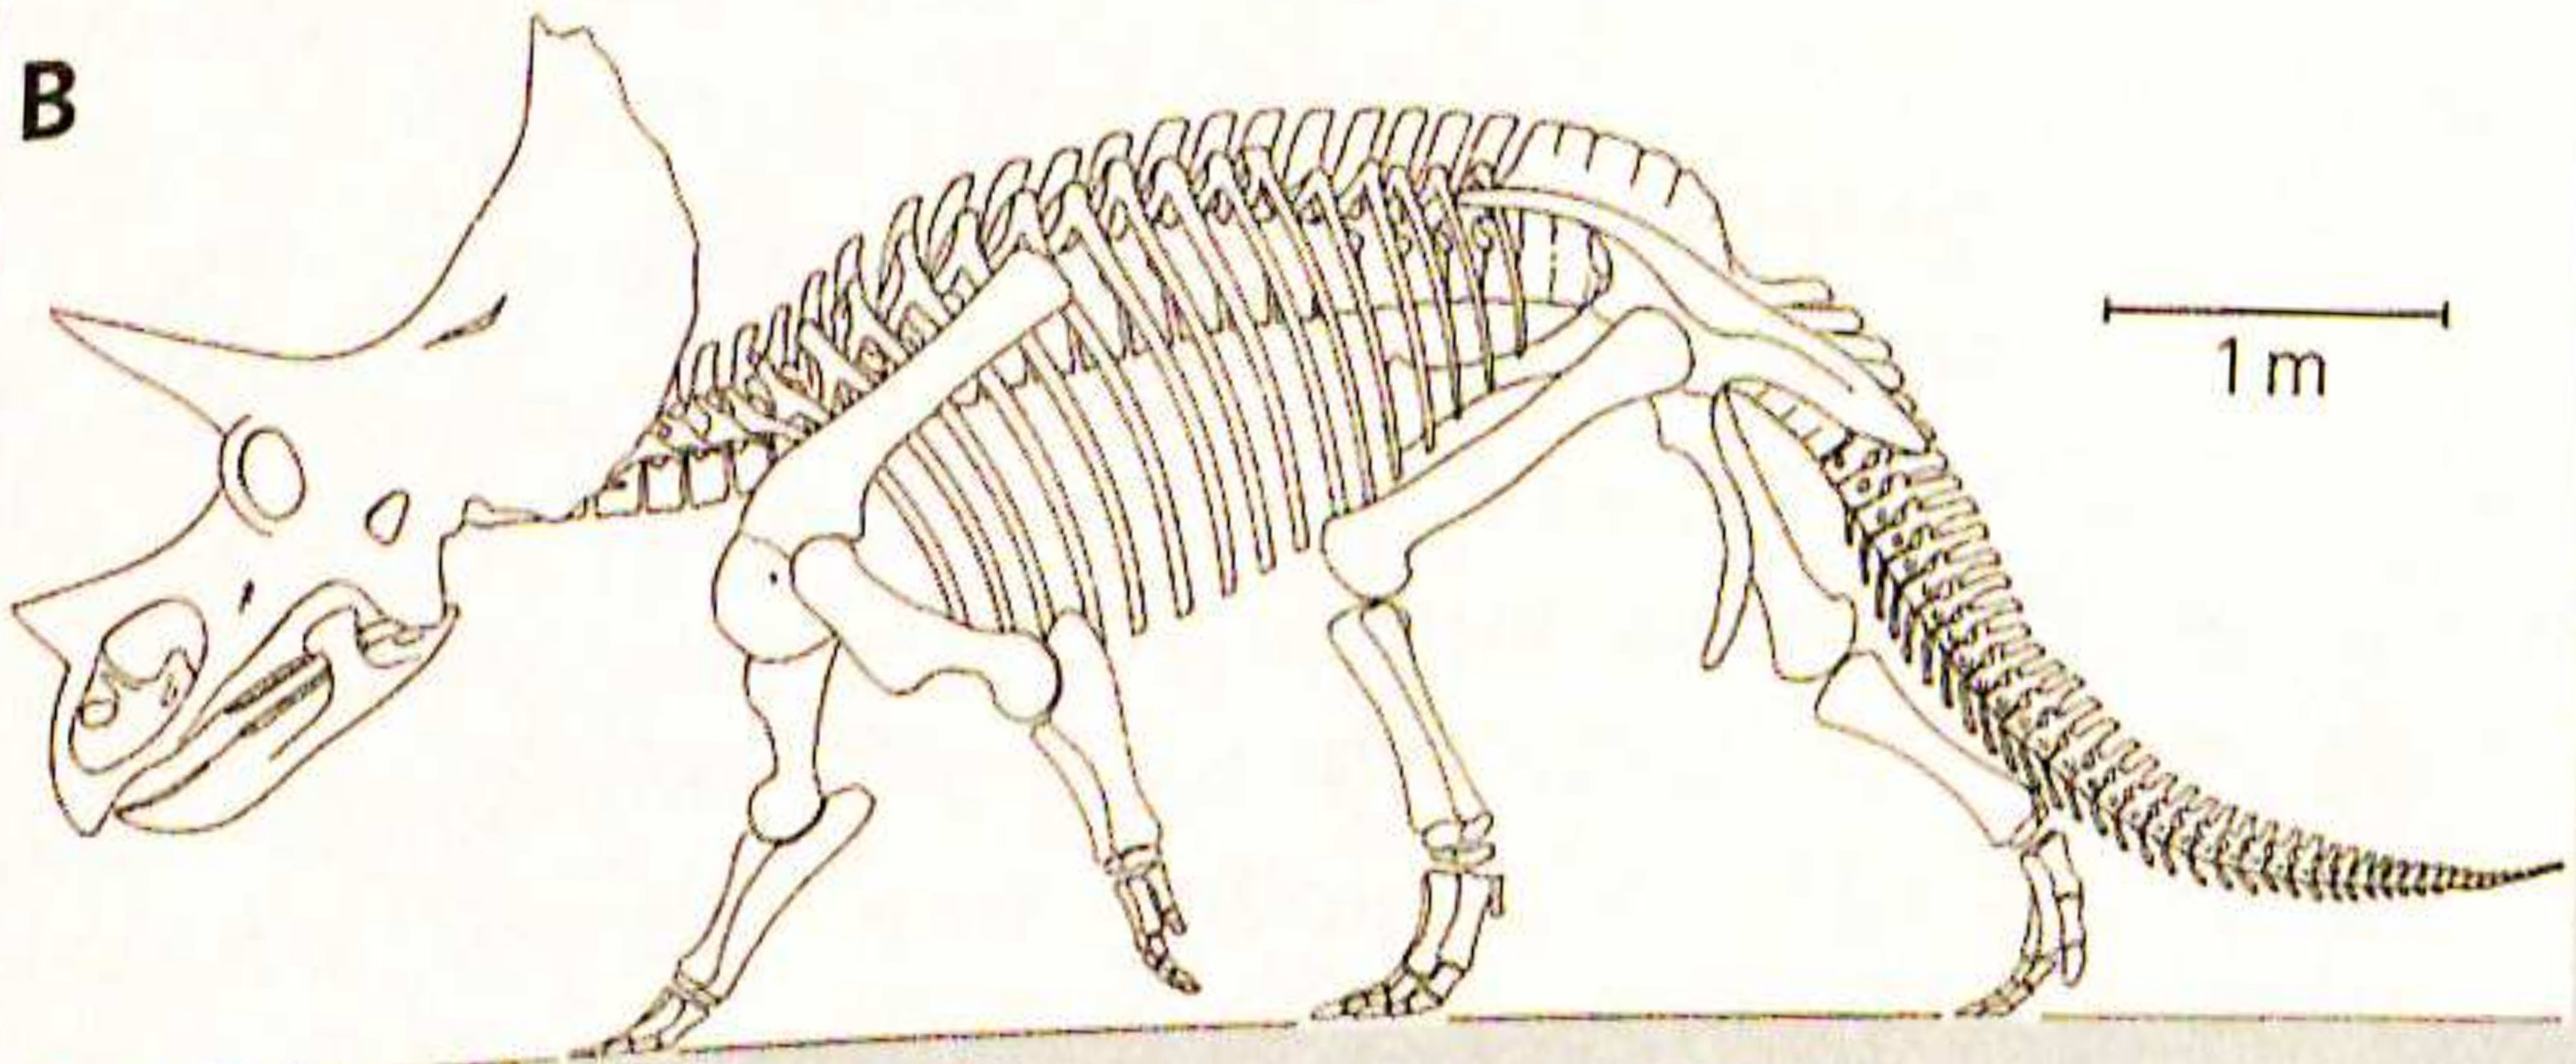
\includegraphics[width=0.2\textwidth]{../PCA/Skelettbilder_klein/Triceratops.jpg}}~
\subfloat[Tyrannosaurus Rex]{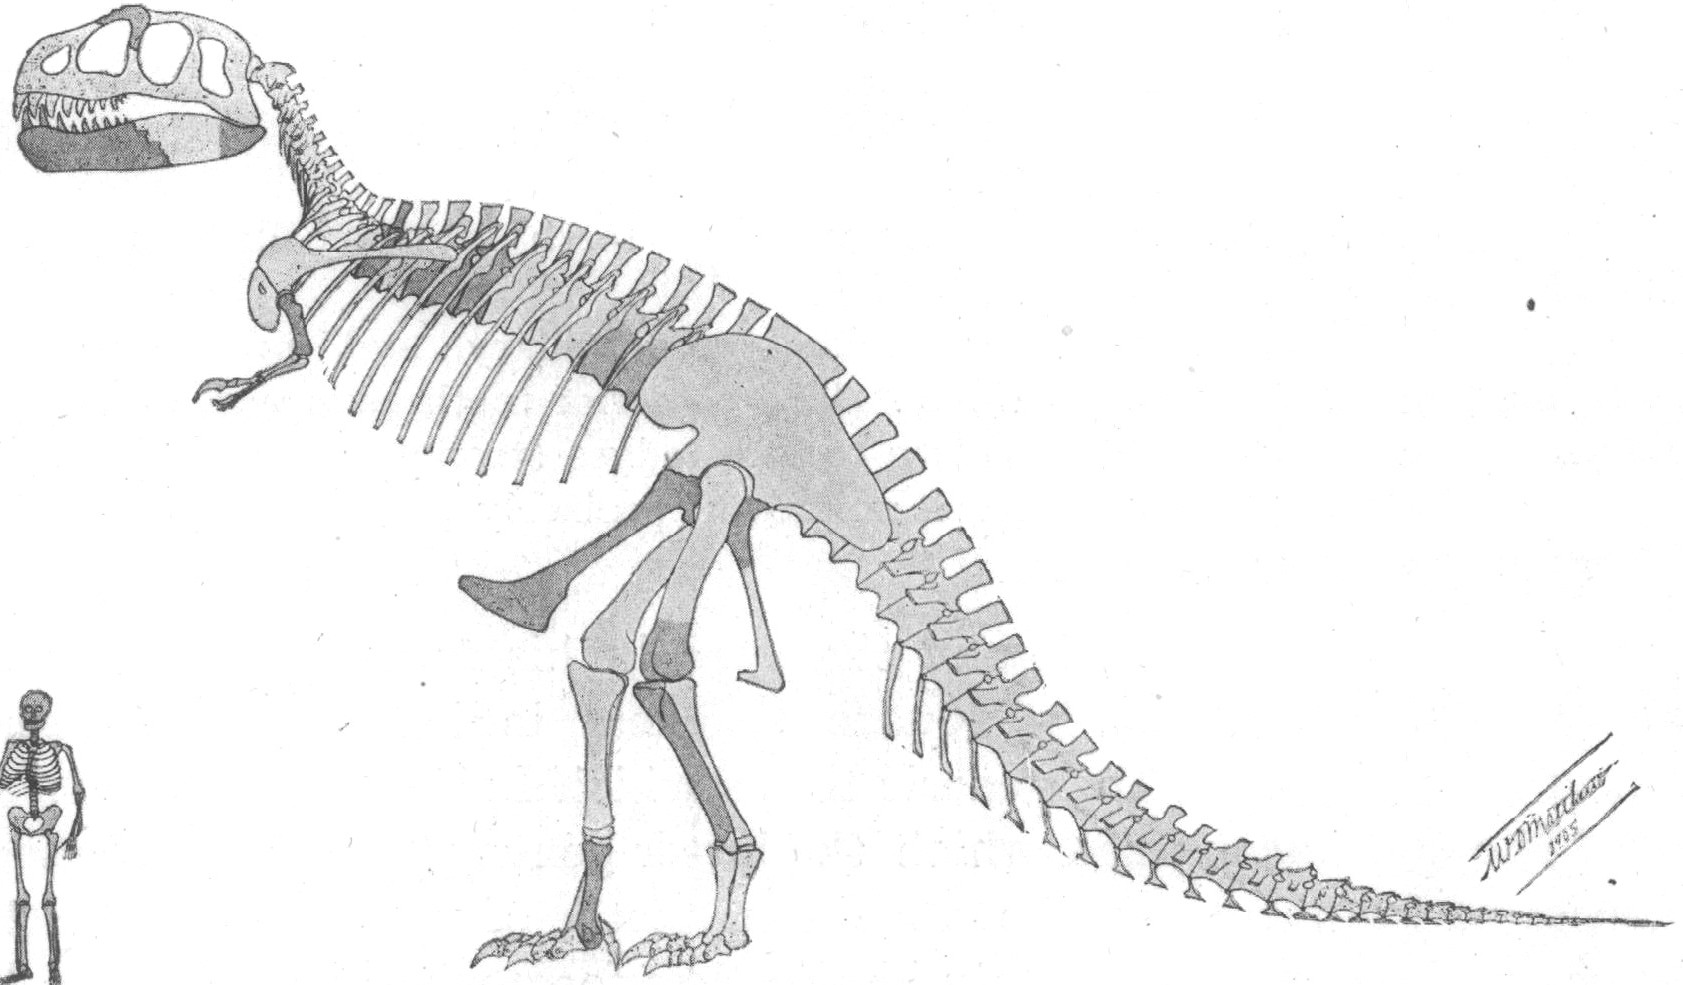
\includegraphics[width=0.2\textwidth]{../PCA/Skelettbilder_klein/Tyrannosaurus_Rex.jpg}}~
\subfloat[Urpferdchen]{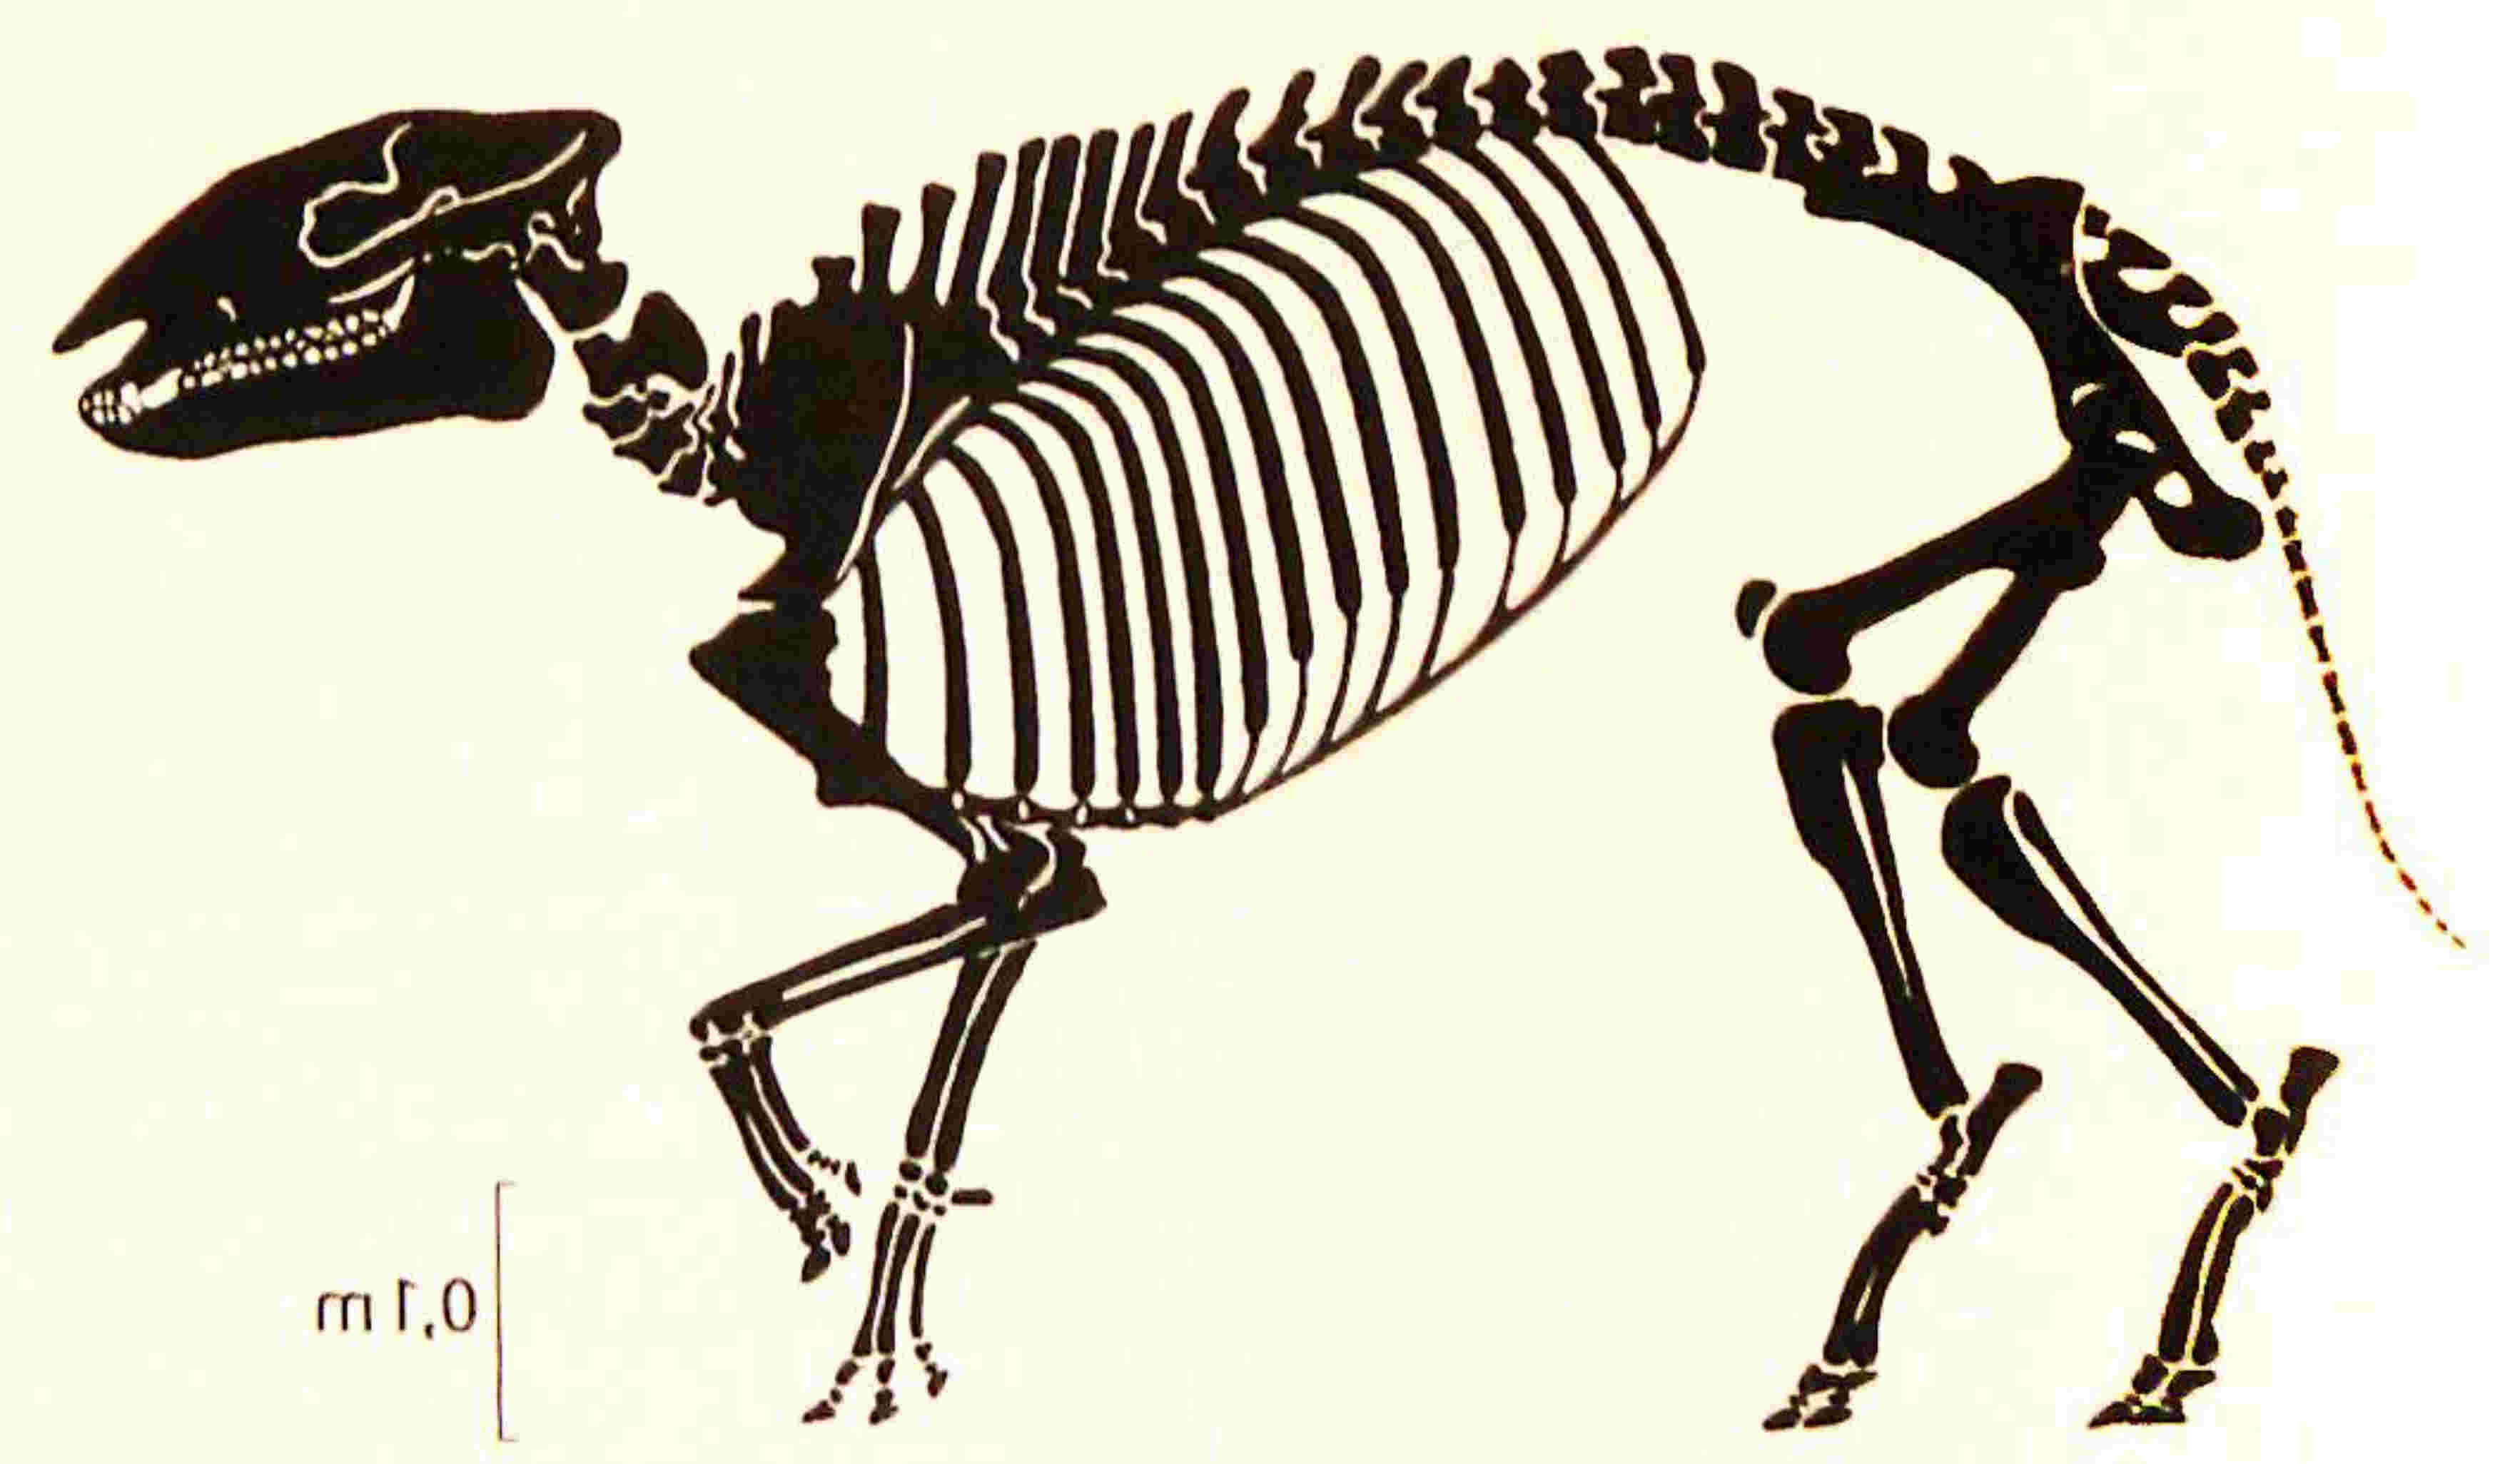
\includegraphics[width=0.2\textwidth]{../PCA/Skelettbilder_klein/Urpferdchen.jpg}}


\caption{Alle Bilder, die als Eingabe für die PCA verwendet wurden.}
\label{all_images}
\end{figure}


 
 \subsection{Gewichte}
 \label{appendix_pca_weight}
 
 \begin{itemize}
  \item Afrikanischer Elefant 4000kg, \url{https://de.upali.ch/gewicht-und-grosse/}
  \item Afrikanischer Strauß bis 135kg, \url{https://de.wikipedia.org/wiki/Afrikanischer_Strau\%C3\%9F}
  \item Amerikanischer Flussbarsch 2kg, \url{http://tierdoku.com/index.php?title=Amerikanischer_Flussbarsch}
  \item Archaeopteryx 1kg, \url{https://de.wikipedia.org/wiki/Archaeopteryx}
  \item Blauwal 120 Tonnen, \url{http://tierdoku.com/index.php?title=Blauwal}, "`das schwerste bekannte Tier der Erdgeschichte"' \url{https://de.wikipedia.org/wiki/Blauwal}
  \item Brachiosaurus 23-44 Tonnen, \url{https://de.wikipedia.org/wiki/Brachiosaurus}
  \item Chamäleon 0,1-2kg, \url{https://www.tierchenwelt.de/echsen/128-chamaeleon.html}
  \item Dimetrodon 250kg, \url{https://de.wikipedia.org/wiki/Dimetrodon}
  \item Dromedar 300-700kg, \url{https://de.wikipedia.org/wiki/Dromedar}
  \item Durschnittsgewicht (Warmblut-)Pferd 600 kg, \url{https://www.reitarena.com/de/blog/blog-post/2015/03/03/das-pferd-grundlegende-fakten.html}
  \item Elster 0,2kg, \url{https://de.wikipedia.org/wiki/Elster}
  \item Forelle 10-50kg (je nach Art), \url{https://de.wikipedia.org/wiki/Forelle}
  \item Frosch 10g, \url{http://www.biologie-schule.de/frosch-steckbrief.php}
  \item Gämse 25-50kg, \url{https://de.wikipedia.org/wiki/G\%C3\%A4mse}
  \item Girafffe bis 2 Tonnen, \url{https://www.tierchenwelt.de/huftiere/73-giraffe.html}
  \item Gnu 140-250kg, \url{https://de.wikipedia.org/wiki/Gnus}
  \item Grönlandwal 50-100 Tonnen, \url{https://de.wikipedia.org/wiki/Gr\%C3\%B6nlandwal}
  \item Ichthyornis 0.3kg, \url{http://dinodata.de/animals/birds/pages_i/ichthyornis.php}
  \item Ichthyosaurus 90kg, \url{https://www.tiere-online.de/sonstige-tiere/dinosaurier/ichthyosaurus/}
  \item Ichthyostega 80kg, \url{https://dinosaurierwelt.com/ichthyostega/}
  \item Kaffernbüffel 350-900kg, \url{https://de.wikipedia.org/wiki/Kaffernb\%C3\%BCffel}
  \item Känguru 2-90kg ,\url{https://de.wikipedia.org/wiki/K\%C3\%A4ngurus}
  \item Kaninchen je nach Art, ganz grob 1kg
  \item Klippschliefer 2-5kg, \url{https://de.wikipedia.org/wiki/Klippschliefer}
  \item Koboldmaki 0,1kg, \url{https://de.wikipedia.org/wiki/Koboldmakis}
  \item Krokodil 100-1000kg, \url{https://de.wikipedia.org/wiki/Krokodile}
  \item Landschildkröte je nach Art, grob 50kg
  \item Ohrenrobbe 25-500kg, \url{https://de.wikipedia.org/wiki/Ohrenrobben}
  \item Panzerspitzmaus 100g ,\url{https://de.wikipedia.org/wiki/Panzerspitzmaus}
  \item Parasaurolophus walkeri 4-5 Tonnen, \url{http://tierdoku.com/index.php?title=Parasaurolophus_walkeri}
  \item Peloneustes philarchus 100kg, \url{https://de.wikipedia.org/wiki/Peloneustes}
  \item Pottwal bis 50 Tonnen, \url{https://de.wikipedia.org/wiki/Pottwal}
  \item Rothirsch 80-350kg, \url{https://de.wikipedia.org/wiki/Rothirsch}
  \item Schlange bis 100kg bei Riesenschlangen, \url{https://de.wikipedia.org/wiki/Schlangen}
  \item Schwan 14kg, \url{https://de.wikipedia.org/wiki/Schw\%C3\%A4ne}
  \item Schwein 100kg, \url{https://de.wikipedia.org/wiki/Hausschwein}
  \item Seehund 100-150kg, \url{https://de.wikipedia.org/wiki/Seehund}
  \item Sinornis 20g, \url{http://dinodata.de/animals/birds/pages_s/sinornis.php}
  \item Stegosaurus 4,5 Tonnen, \url{https://de.wikipedia.org/wiki/Stegosaurus}
  \item Taube je nach Art, grob 1-2kg
  \item Thrinaxodon Reptil "`ein paar Pfund"', \url{https://www.thoughtco.com/thrinaxodon-1091887}
  \item Triceratops 6-12 Tonnen, \url{https://de.wikipedia.org/wiki/Triceratops}
  \item Tyrannosaurus 9 Tonnen, \url{https://de.wikipedia.org/wiki/Tyrannosaurus}
  \item Urpferdchen (Propalaeotherium) 30kg, \url{https://de.wikipedia.org/wiki/Propalaeotherium}
 \end{itemize}
 

% --------------
% Erhobene Werte
% --------------

  \begin{figure}
   \subfloat[Erster Punkt des Halses]{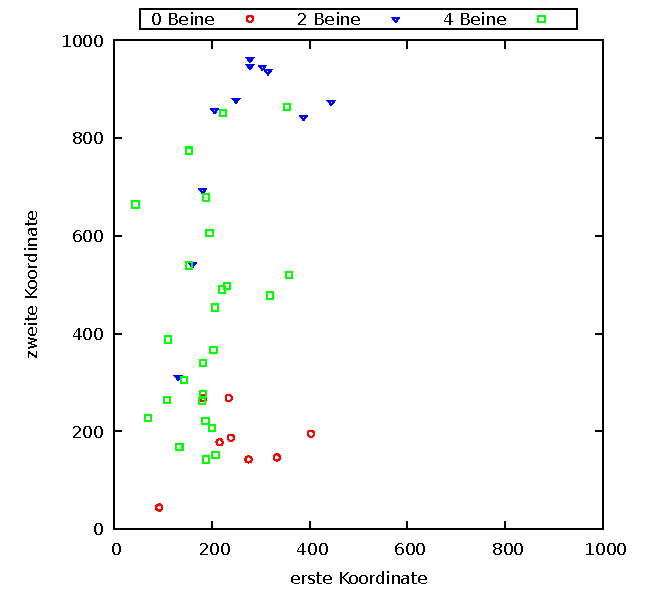
\includegraphics[width=0.3\textwidth]{../PCA/gnuplot/results_with_leg_tag/input_neck1.pdf}}
   \qquad
   \subfloat[Zweiter Punkt des Halses]{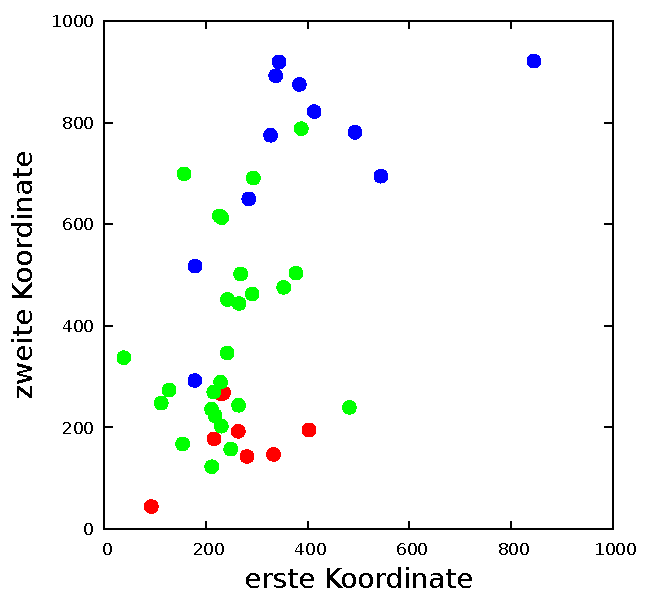
\includegraphics[width=0.3\textwidth]{../PCA/gnuplot/results_with_leg_tag/input_neck2.pdf}}
   \qquad
   \subfloat[Dritter Punkt des Halses]{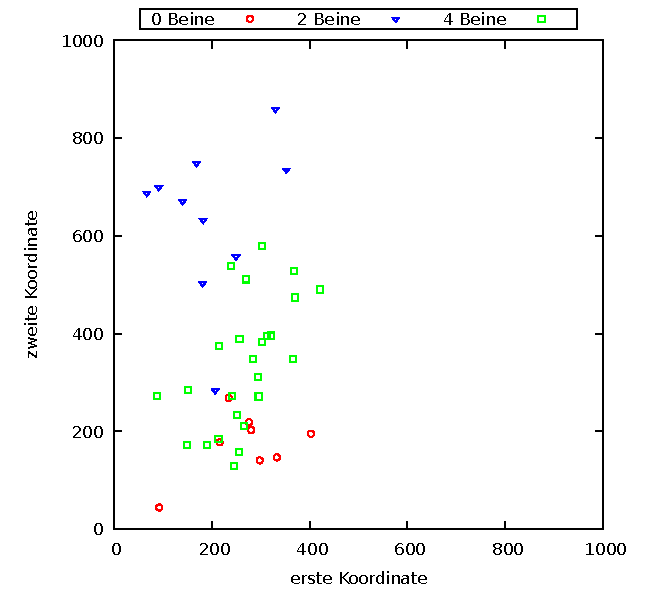
\includegraphics[width=0.3\textwidth]{../PCA/gnuplot/results_with_leg_tag/input_neck3.pdf}}
   \\
   \subfloat[Vierter Punkt des Halses \bzw erster Punkt des Rückens]{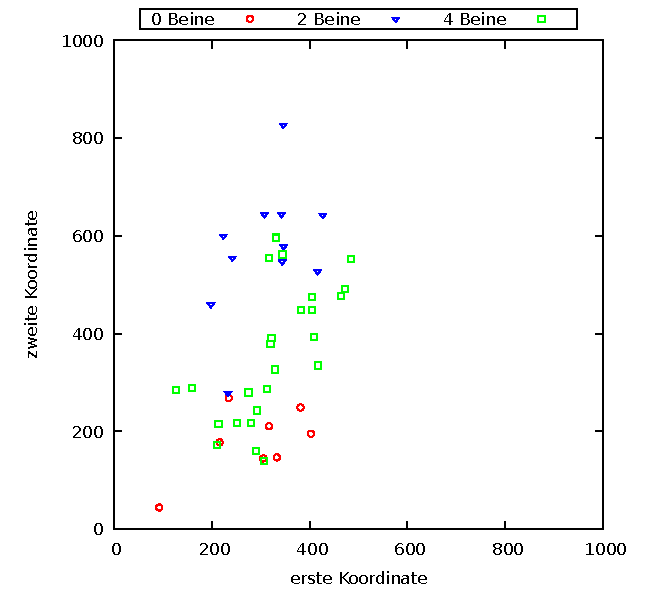
\includegraphics[width=0.3\textwidth]{../PCA/gnuplot/results_with_leg_tag/input_back1.pdf}}
   \qquad
   \subfloat[Zweiter Punkt des Rückens]{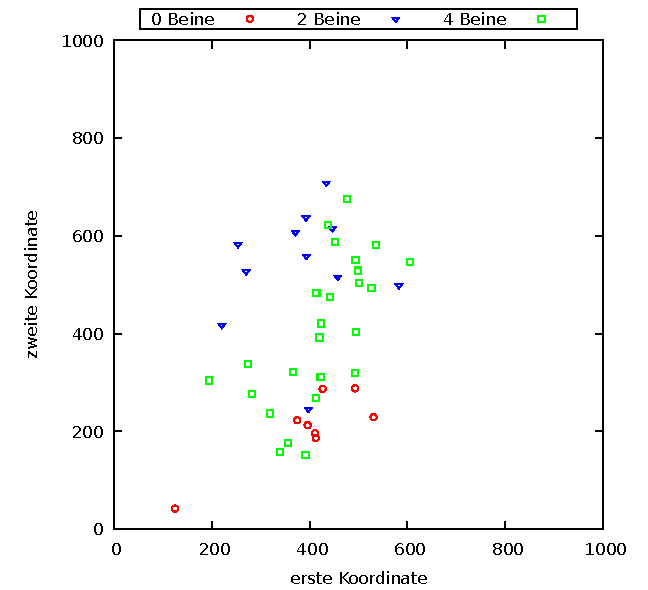
\includegraphics[width=0.3\textwidth]{../PCA/gnuplot/results_with_leg_tag/input_back2.pdf}}
   \qquad
   \subfloat[Dritter Punkt des Rückens]{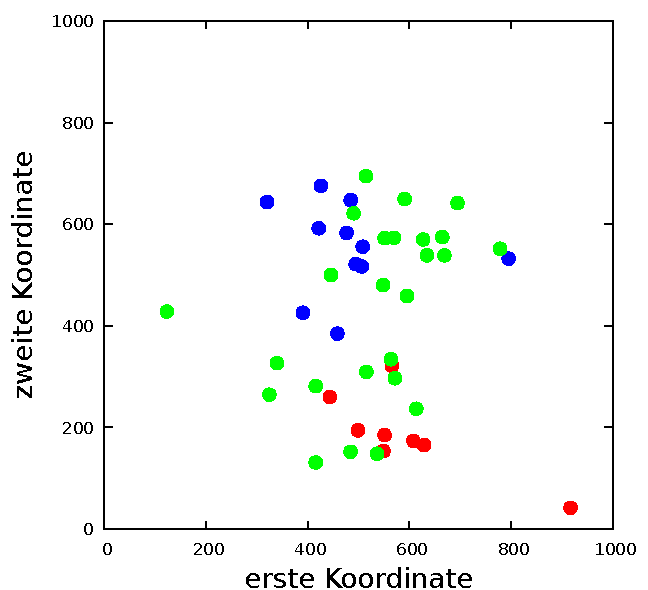
\includegraphics[width=0.3\textwidth]{../PCA/gnuplot/results_with_leg_tag/input_back3.pdf}}
   \\
   \subfloat[Vierter Punkt des Rückens \bzw erster Punkt des Schwanzes]{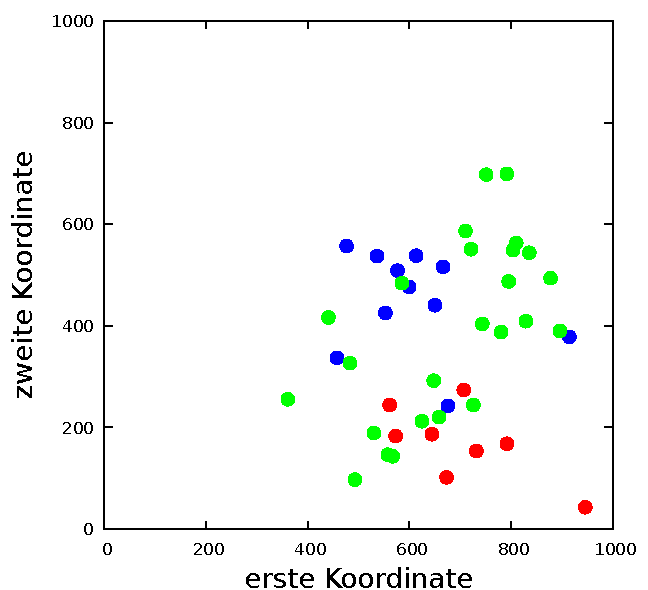
\includegraphics[width=0.3\textwidth]{../PCA/gnuplot/results_with_leg_tag/input_back4.pdf}}
   \qquad
   \subfloat[Zweiter Punkt des Schwanzes]{\includegraphics[width=0.3\textwidth]{../PCA/gnuplot/results_with_leg_tag/input_tail2.pdf}}
   \qquad
   \subfloat[Dritter Punkt des Schwanzes]{\includegraphics[width=0.3\textwidth]{../PCA/gnuplot/results_with_leg_tag/input_tail3.pdf}}
   \\
   \subfloat[Vierter Punkt des Schwanzes]{\includegraphics[width=0.3\textwidth]{../PCA/gnuplot/results_with_leg_tag/input_tail4.pdf}}
   \qquad
   \subfloat[Länge Ober- und Unterarm]{\includegraphics[width=0.3\textwidth]{../PCA/gnuplot/results_with_leg_tag/input_upper+lowerArm.pdf}}
   \qquad
   \subfloat[Länge Unterarm und Hand]{\includegraphics[width=0.3\textwidth]{../PCA/gnuplot/results_with_leg_tag/input_lowerArm+hand.pdf}}
   \phantomcaption
  \end{figure}
  \begin{figure}
   \ContinuedFloat
   \subfloat[Länge Ober- und Unterschenkel]{\includegraphics[width=0.3\textwidth]{../PCA/gnuplot/results_with_leg_tag/input_upper+lowerLeg.pdf}}
   \qquad
   \subfloat[Länge Unterschenkel und Fuß]{\includegraphics[width=0.3\textwidth]{../PCA/gnuplot/results_with_leg_tag/input_lowerLeg+foot.pdf}}
   
   \caption{Erhobene Daten: Punkte der Bézierkurven der Wirbelsäule und Längen der Extremitäten. Bei den Extremitäten ist jeweils gegeneinander abgetragen Ober- und Unterarm, Ober- und Unterschenkel, Unterarm und Hand, Unterschenkel und Fuß. Markiert ist jeweils ob die Datenpunkte $0$ (rot), $2$ (blau) oder $4$ (grün) Beine haben.}
   \label{input_data}
  \end{figure}
  
 \begin{figure}
  \subfloat[lineare Skala]{\includegraphics[width=0.5\textwidth]{../PCA/gnuplot/results_with_leg_tag/input_weight.pdf} \label{gnuplot_weight}}
  \qquad
  \subfloat[logarithmische Skala]{\includegraphics[width=0.5\textwidth]{../PCA/gnuplot/results_with_leg_tag/input_weight_logarithmic.pdf}\label{gnuplot_log_weight}}
  
  \caption{Erhobene Daten: Gewicht. Markiert ist jeweils ob die Datenpunkte $0$ (rot), $2$ (blau) oder $4$ (grün) Beine haben.}
  \label{input_data_weight}
 \end{figure}
 
 %--------------
 % QQ Diagramme
 % ------------

  \begin{figure}
   \subfloat[Erster Punkt des Halses, x-Koordinate]{\includegraphics[width=0.3\textwidth]{../PCA/gnuplot/results_qq_diagrams/QQ_diagram0.pdf}}
   \qquad
   \subfloat[Erster Punkt des Halses, y-Koordinate]{\includegraphics[width=0.3\textwidth]{../PCA/gnuplot/results_qq_diagrams/QQ_diagram1.pdf}}
   \qquad
   \subfloat[Zweiter Punkt des Halses, x-Koordinate]{\includegraphics[width=0.3\textwidth]{../PCA/gnuplot/results_qq_diagrams/QQ_diagram2.pdf}}
   \\
   \subfloat[Zweiter Punkt des Halses, y-Koordinate]{\includegraphics[width=0.3\textwidth]{../PCA/gnuplot/results_qq_diagrams/QQ_diagram3.pdf}}
   \qquad
   \subfloat[Dritter Punkt des Halses, x-Koordinate]{\includegraphics[width=0.3\textwidth]{../PCA/gnuplot/results_qq_diagrams/QQ_diagram4.pdf}}
   \qquad
   \subfloat[Dritter Punkt des Halses, y-Koordinate]{\includegraphics[width=0.3\textwidth]{../PCA/gnuplot/results_qq_diagrams/QQ_diagram5.pdf}}
   \\
   \subfloat[Erster Punkt des Rückens, x-Koordinate]{\includegraphics[width=0.3\textwidth]{../PCA/gnuplot/results_qq_diagrams/QQ_diagram6.pdf}}
   \qquad
   \subfloat[Erster Punkt des Rückens, y-Koordinate]{\includegraphics[width=0.3\textwidth]{../PCA/gnuplot/results_qq_diagrams/QQ_diagram7.pdf}}
   \qquad
   \subfloat[Zweiter Punkt des Rückens, x-Koordinate]{\includegraphics[width=0.3\textwidth]{../PCA/gnuplot/results_qq_diagrams/QQ_diagram8.pdf}}
   \\
   \subfloat[Zweiter Punkt des Rückens, y-Koordinate]{\includegraphics[width=0.3\textwidth]{../PCA/gnuplot/results_qq_diagrams/QQ_diagram9.pdf}}
   \qquad
   \subfloat[Dritter Punkt des Rückens, x-Koordinate]{\includegraphics[width=0.3\textwidth]{../PCA/gnuplot/results_qq_diagrams/QQ_diagram10.pdf}}
   \qquad
   \subfloat[Dritter Punkt des Rückens, y-Koordinate]{\includegraphics[width=0.3\textwidth]{../PCA/gnuplot/results_qq_diagrams/QQ_diagram11.pdf}}
   \phantomcaption
  \end{figure}
  \begin{figure}
   \ContinuedFloat
   \subfloat[Vierter Punkt des Rückens, x-Koordinate]{\includegraphics[width=0.3\textwidth]{../PCA/gnuplot/results_qq_diagrams/QQ_diagram12.pdf}}
   \qquad
   \subfloat[Vierter Punkt des Rückens, y-Koordinate]{\includegraphics[width=0.3\textwidth]{../PCA/gnuplot/results_qq_diagrams/QQ_diagram13.pdf}}
   \qquad
   \subfloat[Zweiter Punkt des Schwanzes, x-Koordinate]{\includegraphics[width=0.3\textwidth]{../PCA/gnuplot/results_qq_diagrams/QQ_diagram14.pdf}}
   \\
   \subfloat[Zweiter Punkt des Schwanzes, y-Koordinate]{\includegraphics[width=0.3\textwidth]{../PCA/gnuplot/results_qq_diagrams/QQ_diagram15.pdf}}
   \qquad
   \subfloat[Dritter Punkt des Schwanzes, x-Koordinate]{\includegraphics[width=0.3\textwidth]{../PCA/gnuplot/results_qq_diagrams/QQ_diagram16.pdf}}
   \qquad
   \subfloat[Dritter Punkt des Schwanzes, y-Koordinate]{\includegraphics[width=0.3\textwidth]{../PCA/gnuplot/results_qq_diagrams/QQ_diagram17.pdf}}
   \\
   \subfloat[Vierter Punkt des Schwanzes, x-Koordinate]{\includegraphics[width=0.3\textwidth]{../PCA/gnuplot/results_qq_diagrams/QQ_diagram18.pdf}}
   \qquad
   \subfloat[Vierter Punkt des Schwanzes, y-Koordinate]{\includegraphics[width=0.3\textwidth]{../PCA/gnuplot/results_qq_diagrams/QQ_diagram19.pdf}}
   
   \caption{Quantil-Quantil-Diagramme für alle Dimensionen der Wirbelsäule}
   \label{qq_diagrams_spine}
  \end{figure}
  \begin{figure}
   \subfloat[Länge Oberarm]{\includegraphics[width=0.3\textwidth]{../PCA/gnuplot/results_qq_diagrams/QQ_diagram22.pdf}}
   \qquad
   \subfloat[Länge Unterarm]{\includegraphics[width=0.3\textwidth]{../PCA/gnuplot/results_qq_diagrams/QQ_diagram23.pdf}}
   \qquad
   \subfloat[Länge Hand]{\includegraphics[width=0.3\textwidth]{../PCA/gnuplot/results_qq_diagrams/QQ_diagram24.pdf}}
   \\
   \subfloat[Länge Oberschenkel]{\includegraphics[width=0.3\textwidth]{../PCA/gnuplot/results_qq_diagrams/QQ_diagram25.pdf}}
   \qquad
   \subfloat[Länge Unterschenkel]{\includegraphics[width=0.3\textwidth]{../PCA/gnuplot/results_qq_diagrams/QQ_diagram26.pdf}}
   \qquad
   \subfloat[Länge Fuß]{\includegraphics[width=0.3\textwidth]{../PCA/gnuplot/results_qq_diagrams/QQ_diagram27.pdf}}

   \caption{Quantil-Quantil-Diagramme für die Dimensionen der Eingabedaten, die zusätzlich zur Wirbelsäule erhoben wurden. Nicht dargestellt ist das binäre Attribut \emph{Flügel} und die Anzahl der Beine mit Bodenkontakt.}
   \label{qq_diagrams_rest}
  \end{figure}
  
  
% ----------------------------
% Mit PCA erzeugte Datenpunkte
% ----------------------------
 
 \begin{figure}
   \centering
   \subfloat[1-, \emph{Flügel} $0,38$, \emph{Beine} $1,6$, \emph{Gewicht} $92$kg]{\includegraphics[width=0.45\textwidth]{../PCA/sqrtEV_log_weight_downscaled_wings_legs_and_weight/EV1_neg.jpg}}
   \qquad
   \subfloat[1+, \emph{Flügel} $-0,057$, \emph{Beine} $1,2$, \emph{Gewicht} $94$kg]{\includegraphics[width=0.45\textwidth]{../PCA/sqrtEV_log_weight_downscaled_wings_legs_and_weight/EV1_pos.jpg}}
   \\
   \subfloat[2-, \emph{Flügel} $0,014$, \emph{Beine} $1,4$, \emph{Gewicht} $94$kg]{\includegraphics[width=0.45\textwidth]{../PCA/sqrtEV_log_weight_downscaled_wings_legs_and_weight/EV2_neg.jpg}}
   \qquad
   \subfloat[2+, \emph{Flügel} $0,3$, \emph{Beine} $1,3$, \emph{Gewicht} $93$kg]{\includegraphics[width=0.45\textwidth]{../PCA/sqrtEV_log_weight_downscaled_wings_legs_and_weight/EV2_pos.jpg}}
   \\
   \subfloat[3-, \emph{Flügel} $0,11$, \emph{Beine} $1,6$, \emph{Gewicht} $93$kg]{\includegraphics[width=0.45\textwidth]{../PCA/sqrtEV_log_weight_downscaled_wings_legs_and_weight/EV3_neg.jpg}}
   \qquad
   \subfloat[3+, \emph{Flügel} $0,21$, \emph{Beine} $1,2$, \emph{Gewicht} $93$kg]{\includegraphics[width=0.45\textwidth]{../PCA/sqrtEV_log_weight_downscaled_wings_legs_and_weight/EV3_pos.jpg}}
   \phantomcaption
 \end{figure}
 \begin{figure}
   \ContinuedFloat
   \centering
   \subfloat[4-, \emph{Flügel} $0,3$, \emph{Beine} $1$, \emph{Gewicht} $92$kg]{\includegraphics[width=0.45\textwidth]{../PCA/sqrtEV_log_weight_downscaled_wings_legs_and_weight/EV4_neg.jpg}}
   \qquad
   \subfloat[4+, \emph{Flügel} $0,022$, \emph{Beine} $1,8$, \emph{Gewicht} $94$kg]{\includegraphics[width=0.45\textwidth]{../PCA/sqrtEV_log_weight_downscaled_wings_legs_and_weight/EV4_pos.jpg}}
   \\
   \subfloat[5-, \emph{Flügel} $0,08$, \emph{Beine} $1,6$, \emph{Gewicht} $93$kg]{\includegraphics[width=0.45\textwidth]{../PCA/sqrtEV_log_weight_downscaled_wings_legs_and_weight/EV5_neg.jpg}}
   \qquad
   \subfloat[5+, \emph{Flügel} $0,24$, \emph{Beine} $1,2$, \emph{Gewicht} $93$kg]{\includegraphics[width=0.45\textwidth]{../PCA/sqrtEV_log_weight_downscaled_wings_legs_and_weight/EV5_pos.jpg}}
   \\
   \subfloat[6-, \emph{Flügel} $0,21$, \emph{Beine} $1,5$, \emph{Gewicht} $92$kg]{\includegraphics[width=0.45\textwidth]{../PCA/sqrtEV_log_weight_downscaled_wings_legs_and_weight/EV6_neg.jpg}}
   \qquad
   \subfloat[6+, \emph{Flügel} $0,11$, \emph{Beine} $1,3$, \emph{Gewicht} $98$kg]{\includegraphics[width=0.45\textwidth]{../PCA/sqrtEV_log_weight_downscaled_wings_legs_and_weight/EV6_pos.jpg}}
   
   \caption{Datenpunkte im PCA-Koordinatensystem. Eine Koordinate nimmt den Wert der positiven (+) \bzw negativen (-) Standardabweichung in die entsprechende Richtung an, alle anderen sind null. Von oben nach unten sind die Ergebnisse für den größten (1) bis zum sechstgrößten (6) Eigenwert dargestellt. \emph{Beine} steht für \emph{Beine mit Bodenkontakt}.}
   \label{pca_results_sqrtEV}
  \end{figure}


\end{document}
